\documentclass[final]{beamer}
%% \title{Energy and Growth, History and Dynamics}
%\title{Economic development with unlimited supplies of energy:
%\\The English Industrial Revolution and modern economic growth}

\title{China -- the empire that did not bark: the economics of a failed attempt at modern economic growth}
\author{ASA Sociology of Development conference\\University of Utah\\October 2013 
\newline
	\\Stephen C. Bannister\\
	Department of Economics\\
	University of Utah\\
	Salt Lake City, Utah 84112\\
	USA\\
	\href{mailto:steve.bannister@econ.utah.edu}{steve.bannister@econ.utah.edu}\\
	}

%\date{Drafts May 2012,}
\date{}
\usepackage[latin1]{inputenc}
%\usepackage[english]{babel}
\usepackage{amsmath}
\usepackage{amsfonts}
\usepackage{txfonts}
\usepackage{amssymb}
\usepackage{pgfpages}
\usepackage{booktabs}
\usepackage{longtable}

\usetheme{Darmstadt}
\usecolortheme{beaver}

\usepackage{chngpage}
%\usepackage{pdfpages}
\usepackage{graphicx}
%\usepackage[lofdepth,lotdepth,position=bottom]{subfig}
\usepackage{caption}
%\usepackage{draftwatermark}

\usepackage{verbatim}
%\usepackage{underscore}
%\linespread{1.9}	% remove for single, 1.3 for 1.5 and 1.6 for 2.0. use this setting for print editing

\usepackage{glossaries}

\graphicspath{{../images/}}

%\textwidth{7.5in}
%\addtolength{\textwidth}{1.0in} 
%\addtolength{\oddsidemargin}{-0.5in} 
%\addtolength{\evensidemargin}{-0.5in} 
%\addtolength{\textheight}{1.25in}
%\addtolength{\topmargin}{-0.75in}

\setbeamertemplate{navigation symbols}{} %no nav symbols

\usepackage{hyperref}

%\makeglossaries

%\loadglsentries{glossary.tex}

%\setcounter{secnumdepth}{4}%to number paragraphs so can ref them?

\begin{document}

%\SetWatermarkLightness{0.93}
%\SetWatermarkScale{1}

	\maketitle
	\nocite{*}
%	\bibliographystyle{E:/LaTeX-Portable/MikTex-Portable/bibtex/bst/base/IEEEanot}

	\bibliographystyle{E:/LaTeX-Portable/MikTex-Portable/bibtex/bst/base/plain-annote}
%	\bibliographystyle{plain}


\section{Main}

\begin{frame}
\frametitle{The Issue: Why not China? (``Natural'' experiment)}\pause
\begin{itemize}
\item The majority view is that, principally and uniquely, cultural/institutional exceptionalism sparked the English Industrial Revolution (EIR)\\ \pause 
\item Further, the majority claim is that China failed for the same reasons that England succeeded\\ \pause
\item My claim is that \textit{both} views are wrong, have caused a misinterpreted history, and have thus misled development economists, especially in the case of China's failed attempt at an industrial revolution\\ \pause
\item Instead, the data support a Chinese history of one \textbf{\textit{energy}} revolution that was necessary, but not sufficient, to cause a second bigger, sufficient, one. The English accomplished both\\ \pause 
\item In \textbf{each} case the same \textit{economic} explanations are sufficient\\
\end{itemize}
\end{frame}

\begin{frame}
\frametitle{Global Context (Source: Maddison): a Western Bubble?}
\begin{figure}[p!]
%\caption{World GDP and population}
\label{fig:worldContext}
%		\centerline{
		\mbox{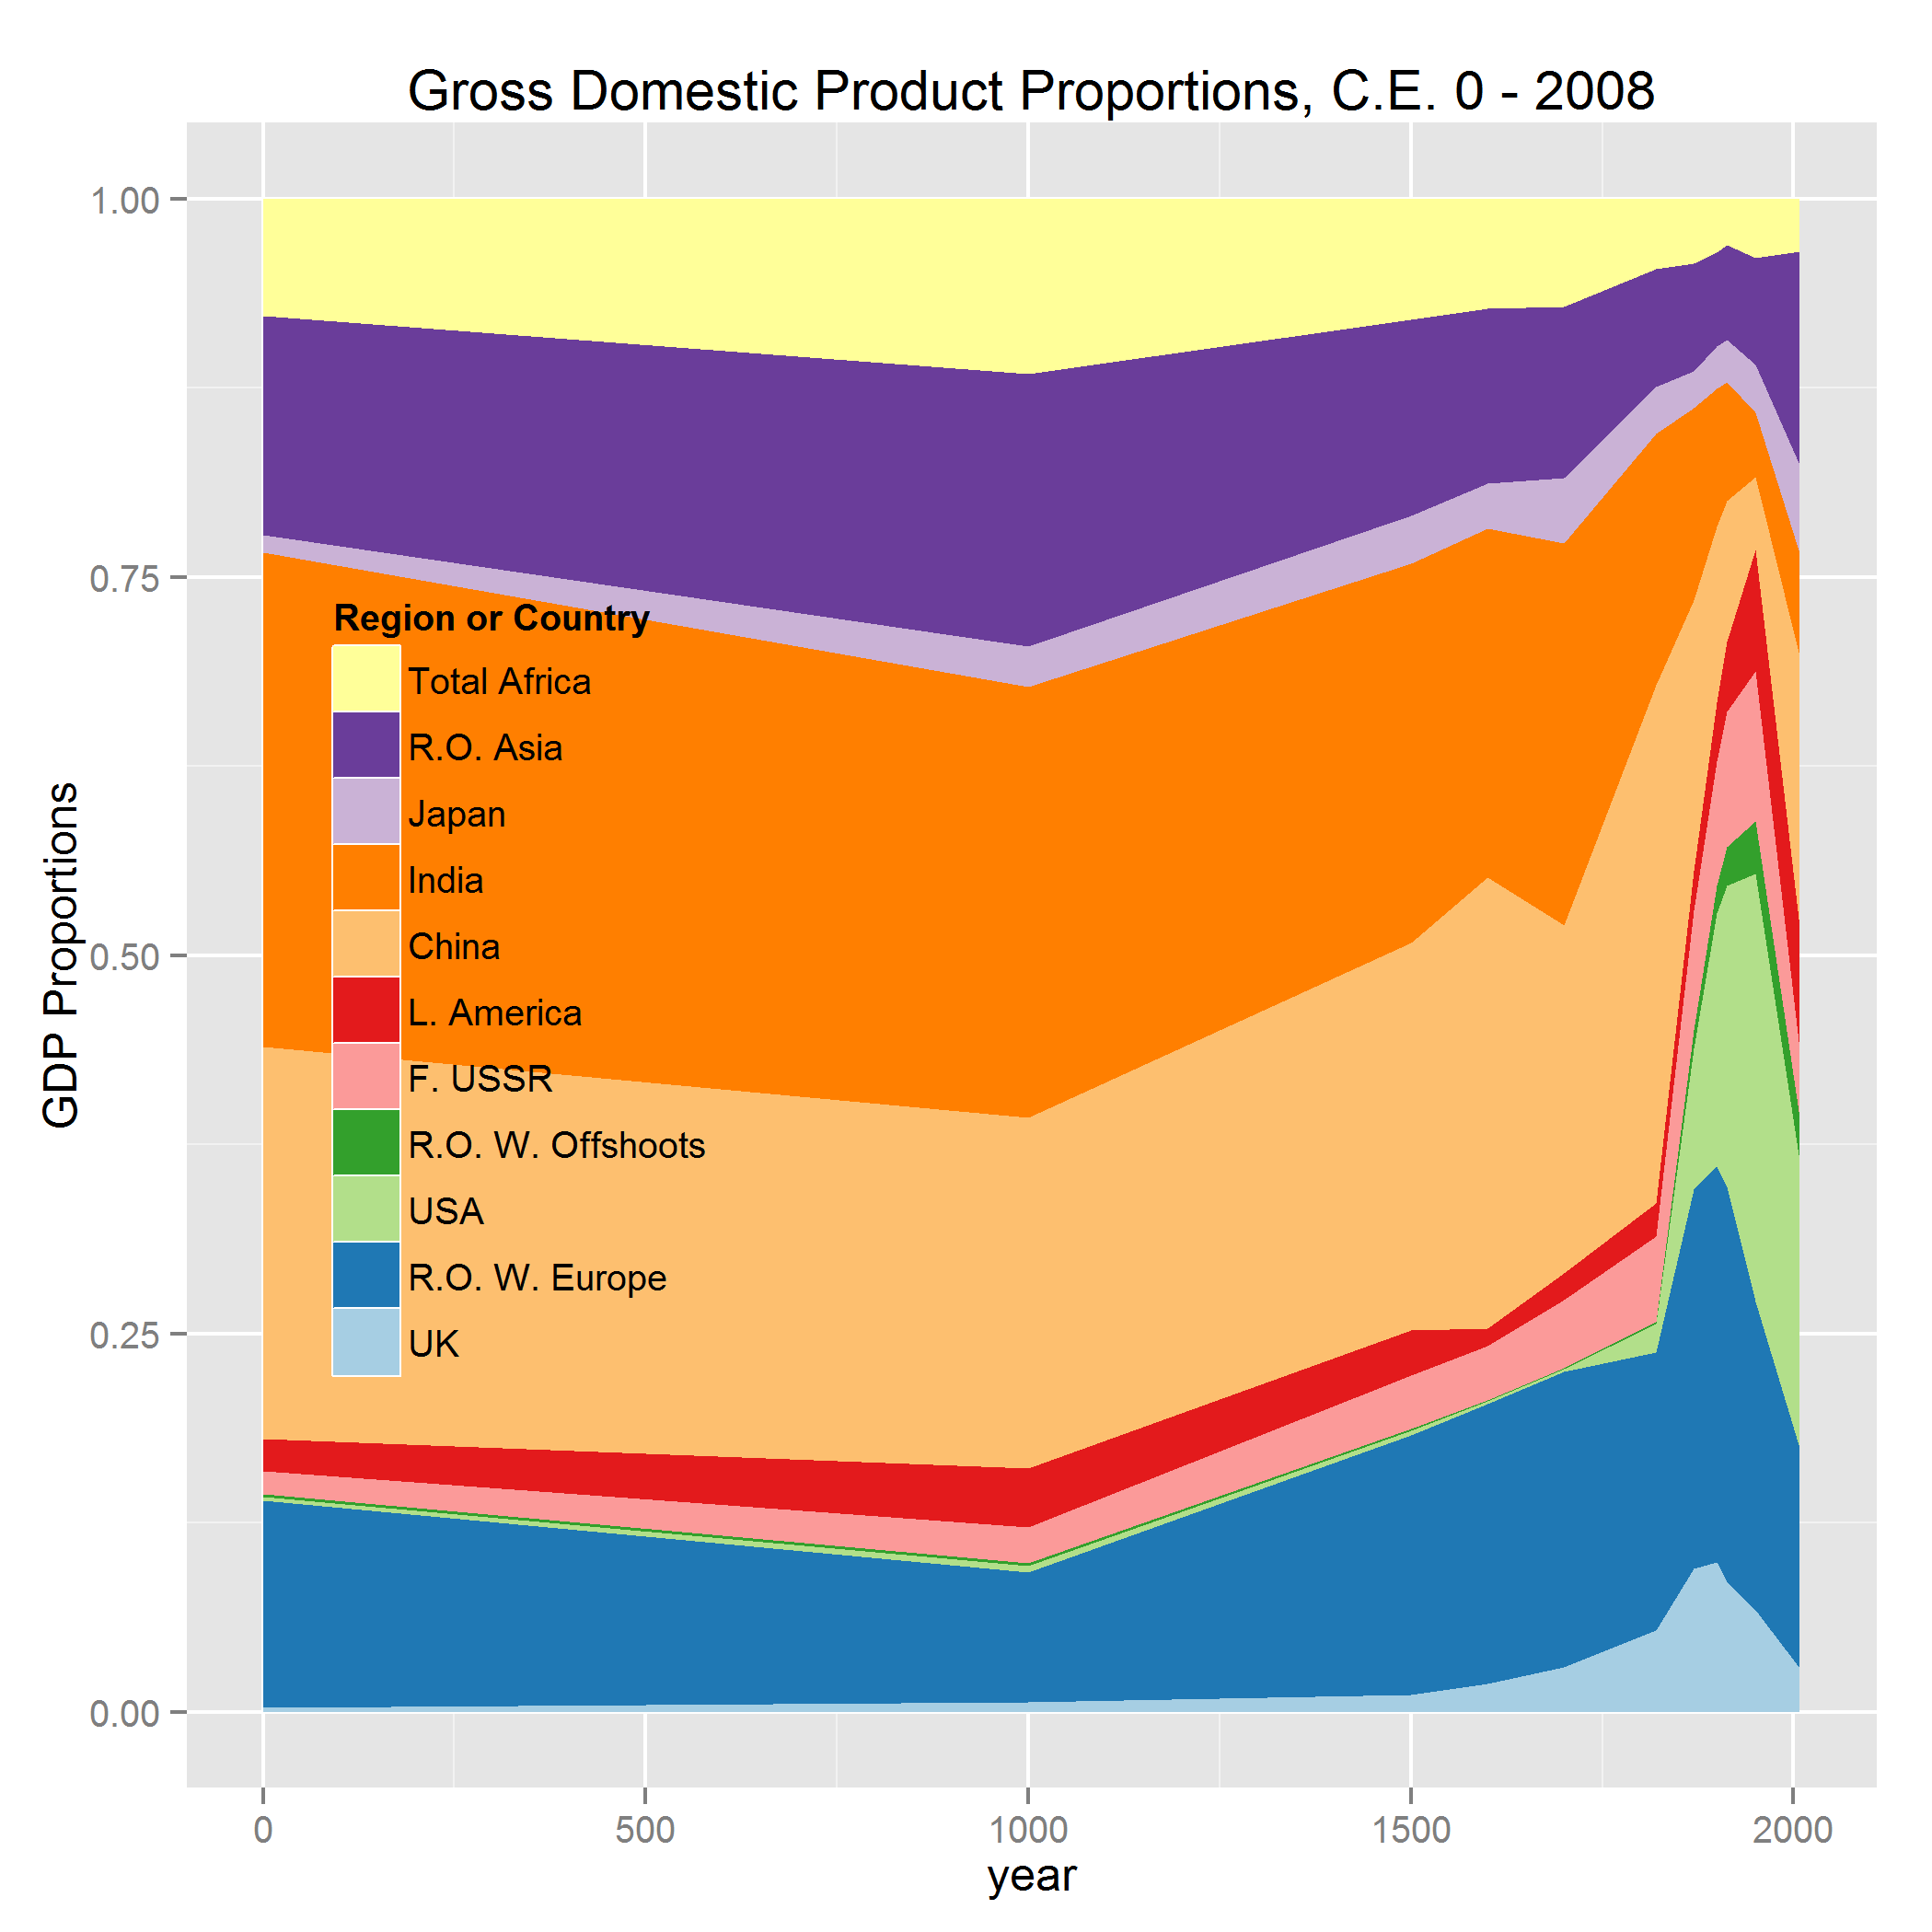
\includegraphics[height=0.43\textheight]{maddisonreggdppct}}
		\mbox{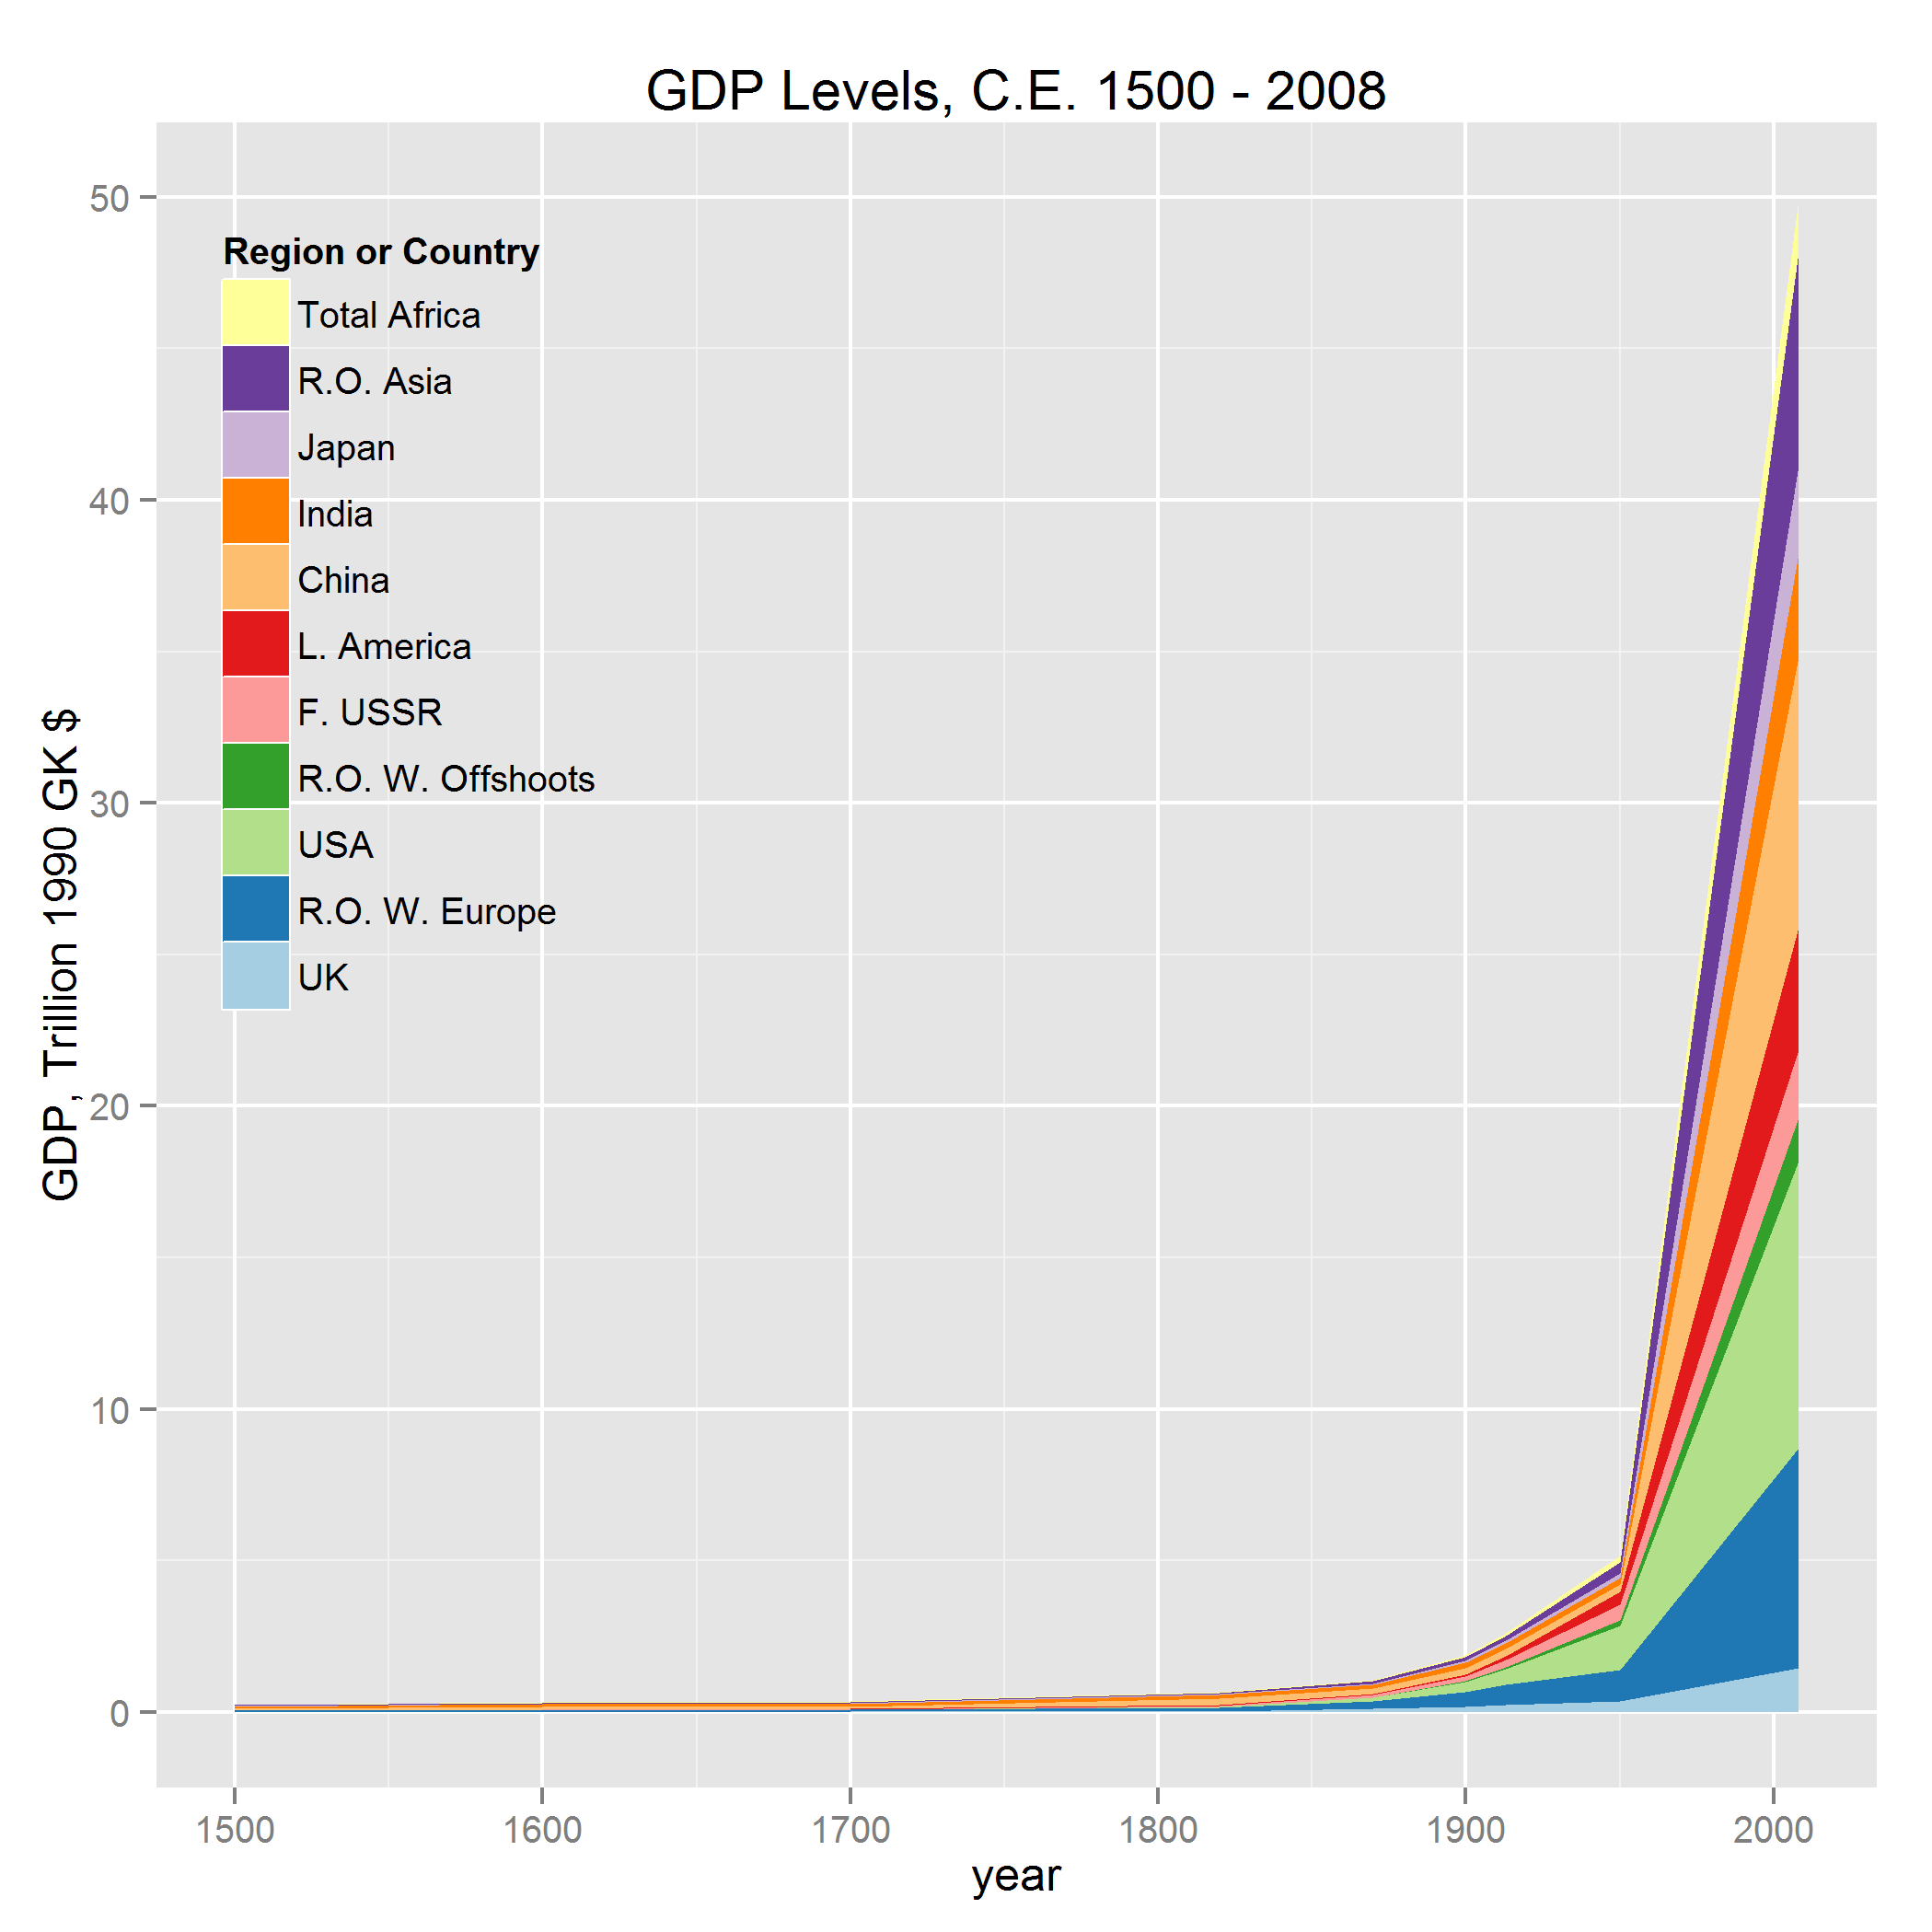
\includegraphics[height=0.43\textheight]{maddisonreggdplevels}}\\
		\mbox{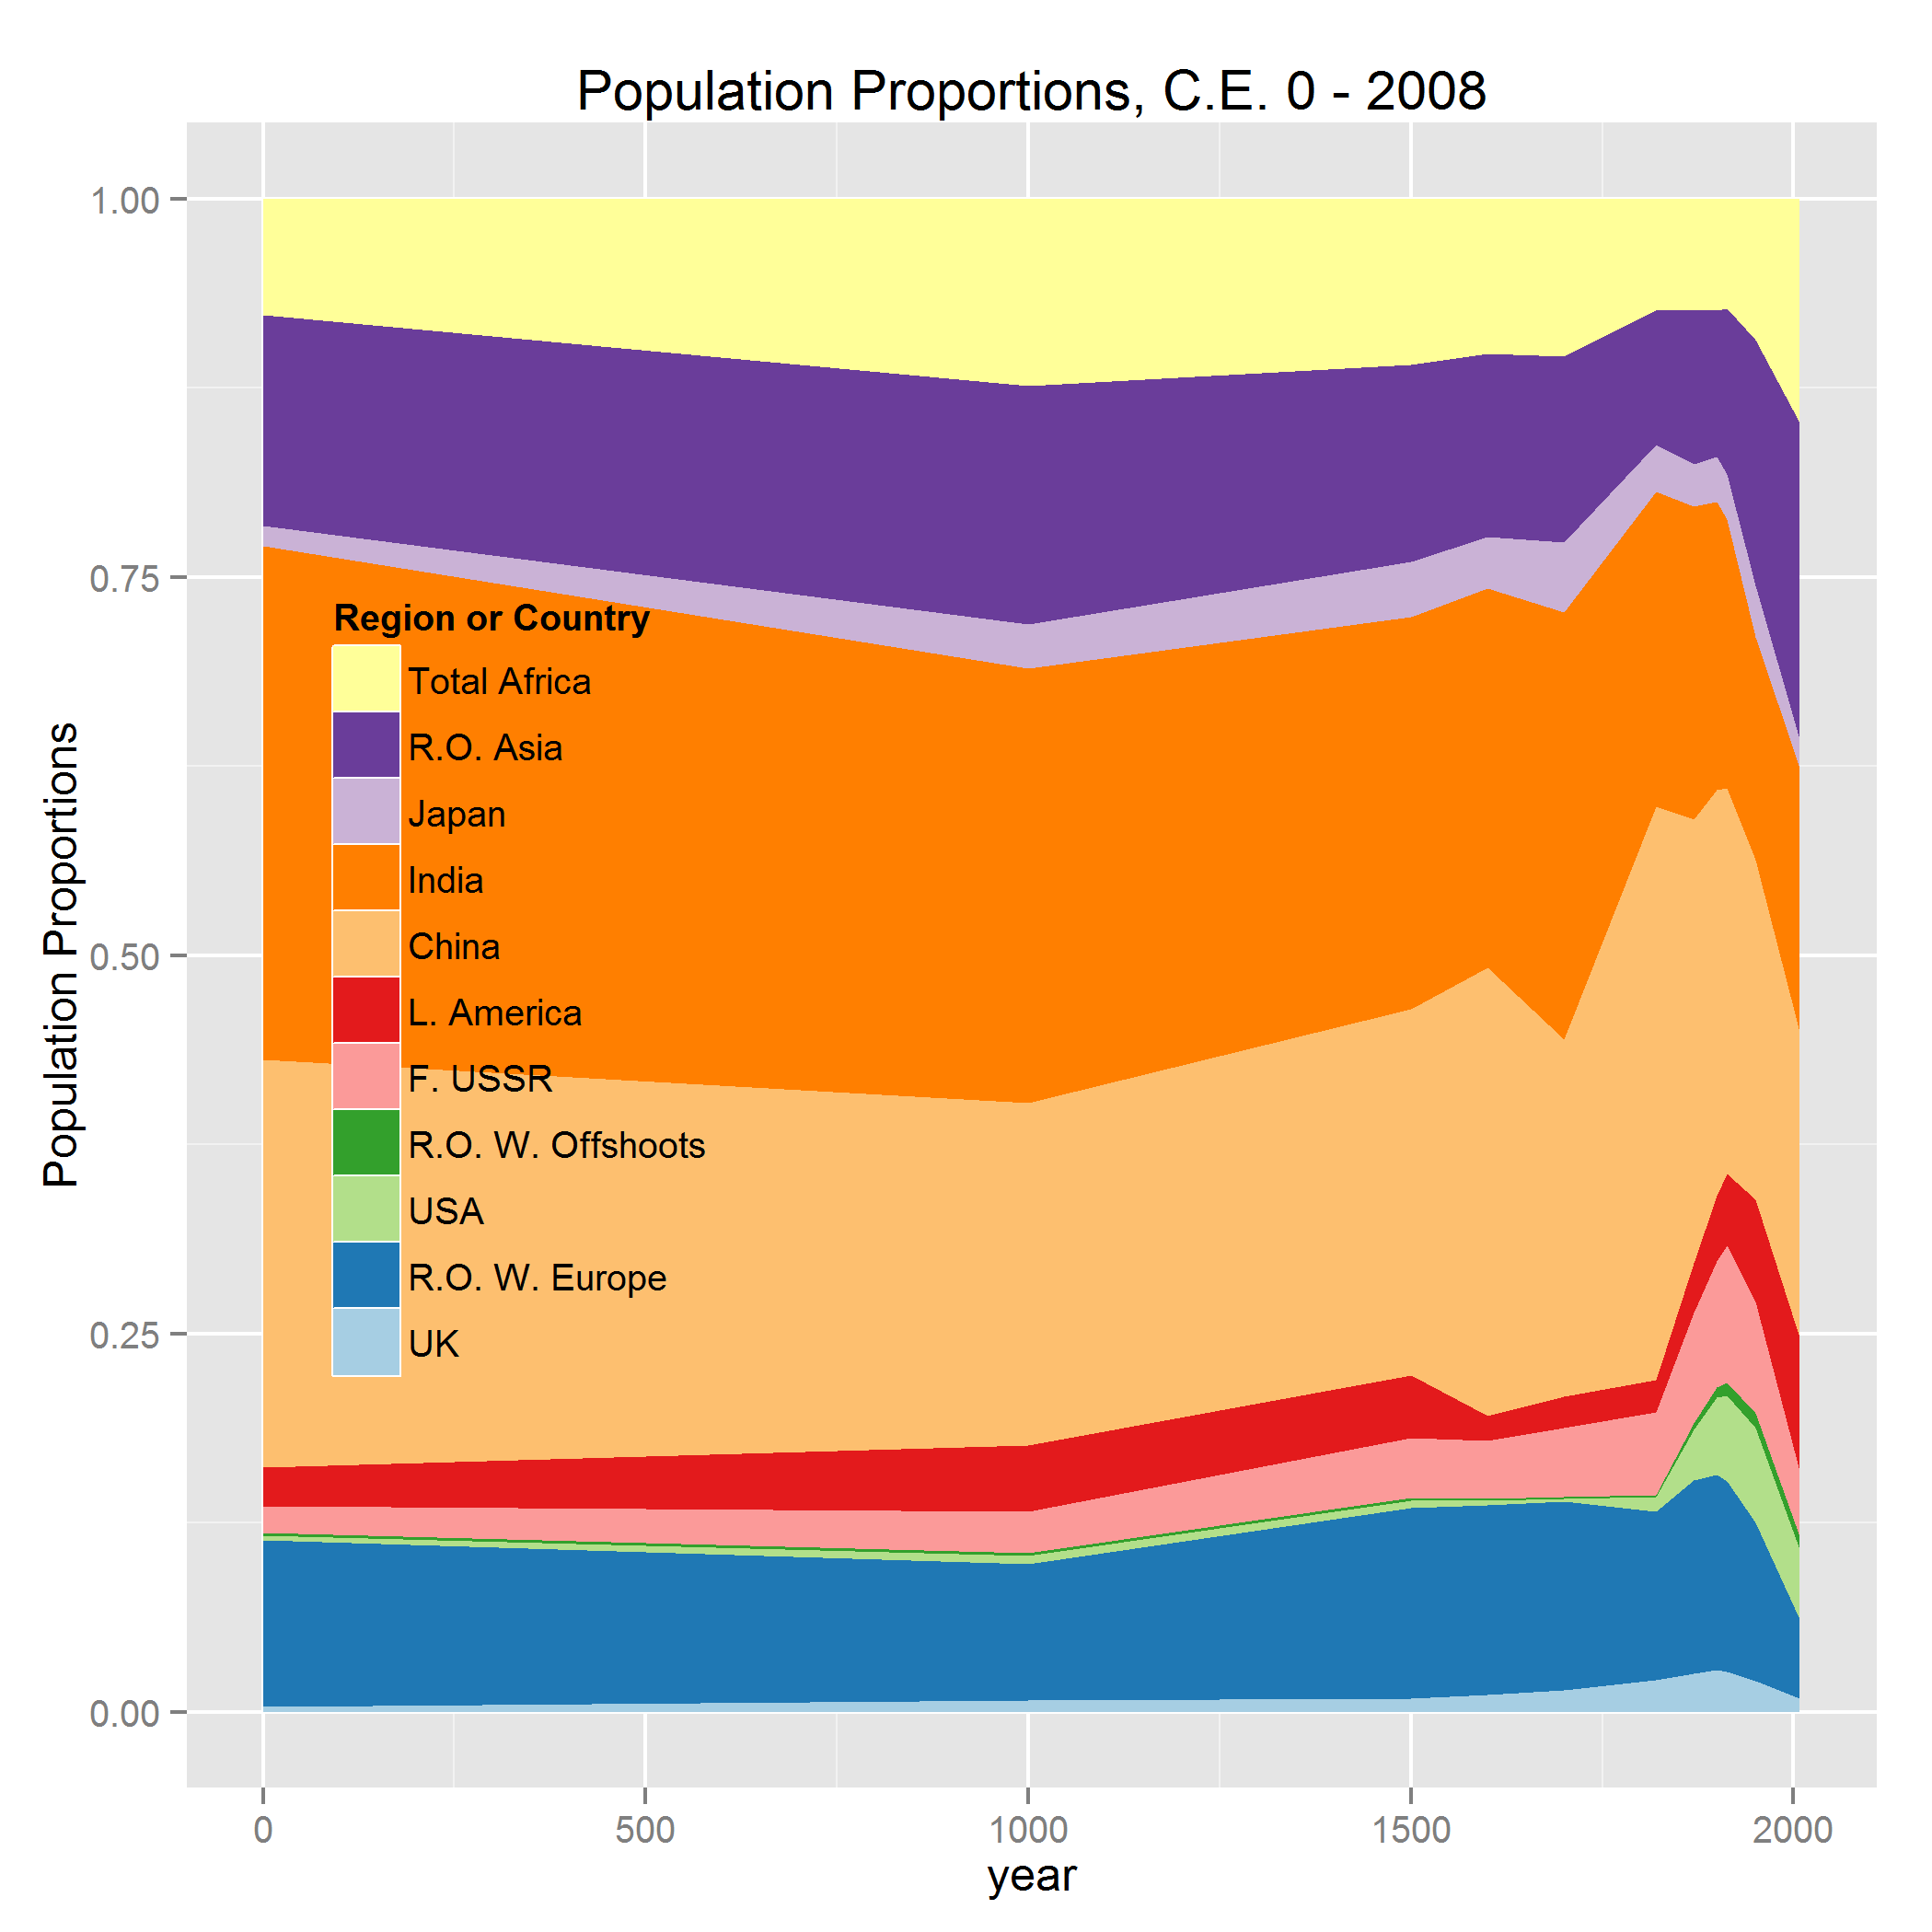
\includegraphics[height=0.43\textheight]{maddisonregpoppct}}
		\mbox{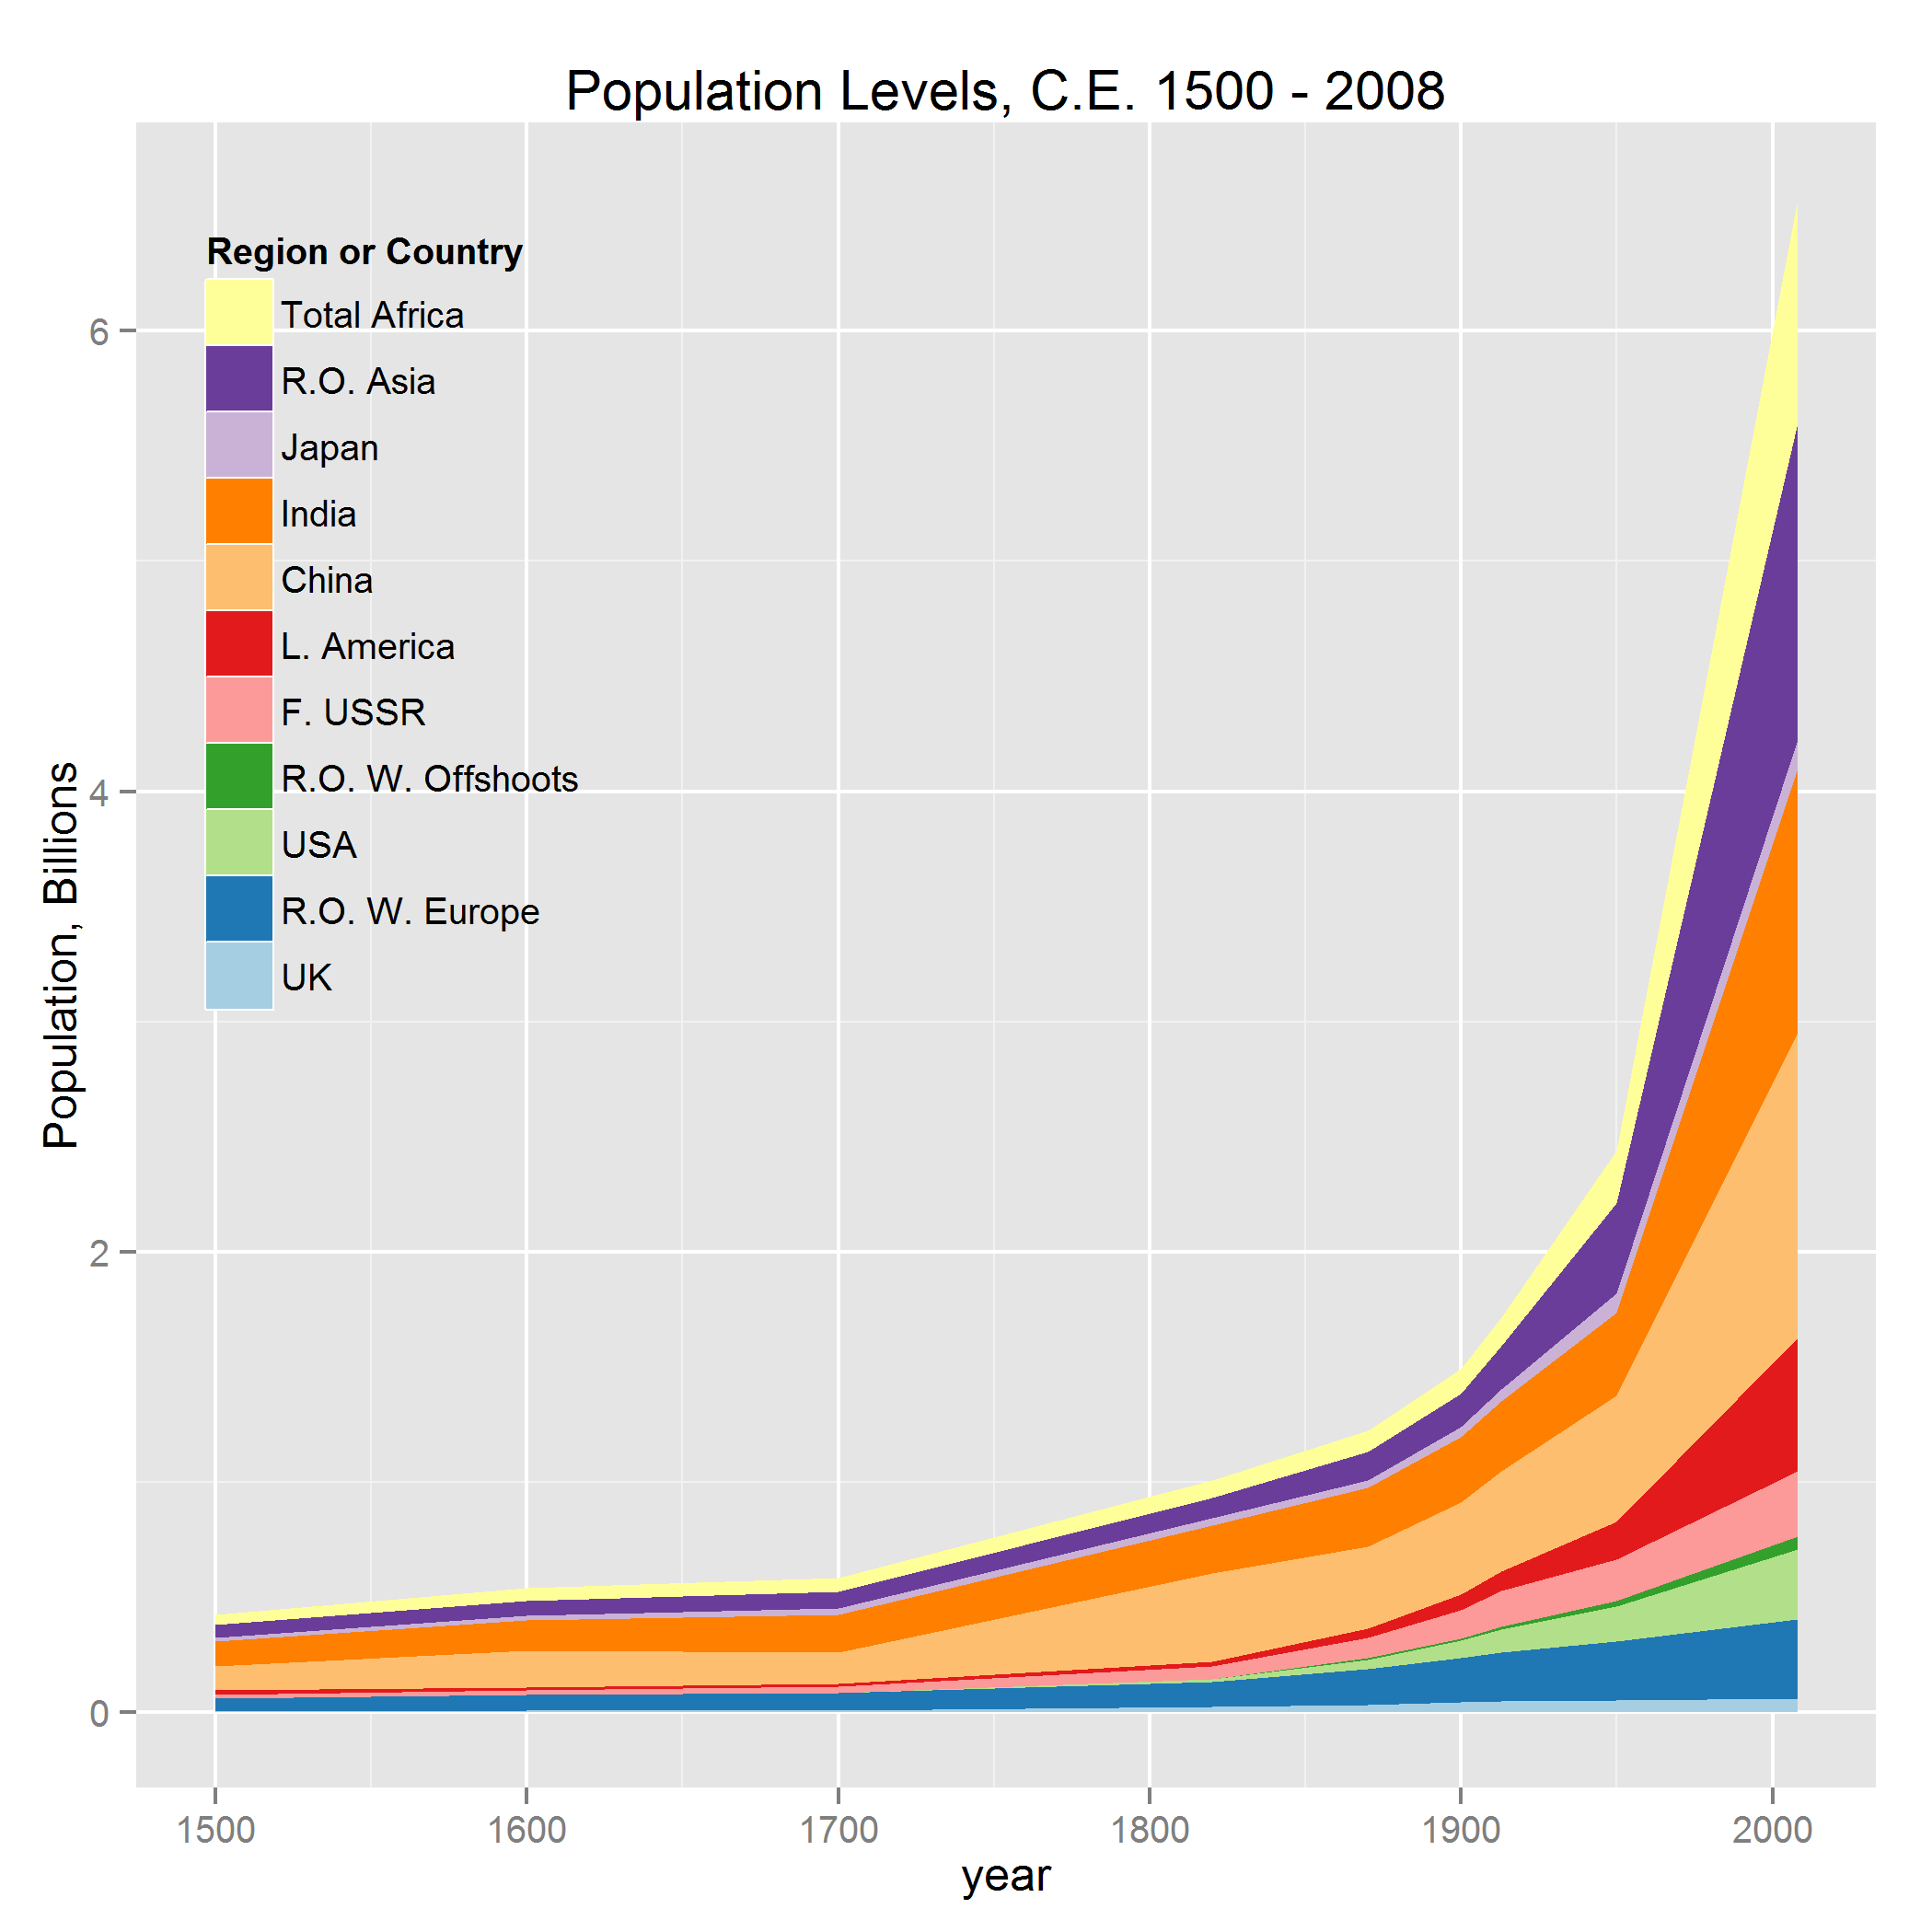
\includegraphics[height=0.43\textheight]{maddisonregpoplevels}}
%		}
\end{figure} %\vspace*{-0.4in}
\end{frame}

\begin{frame}
\frametitle{The English data -- two energy revolutions that \textit{\textbf{were}} the EIR}
\begin{figure}[p!]
%\caption{Scatterplot of energy consumption vs. GDP}
\label{fig:scatterplot}
		\centerline{
		\mbox{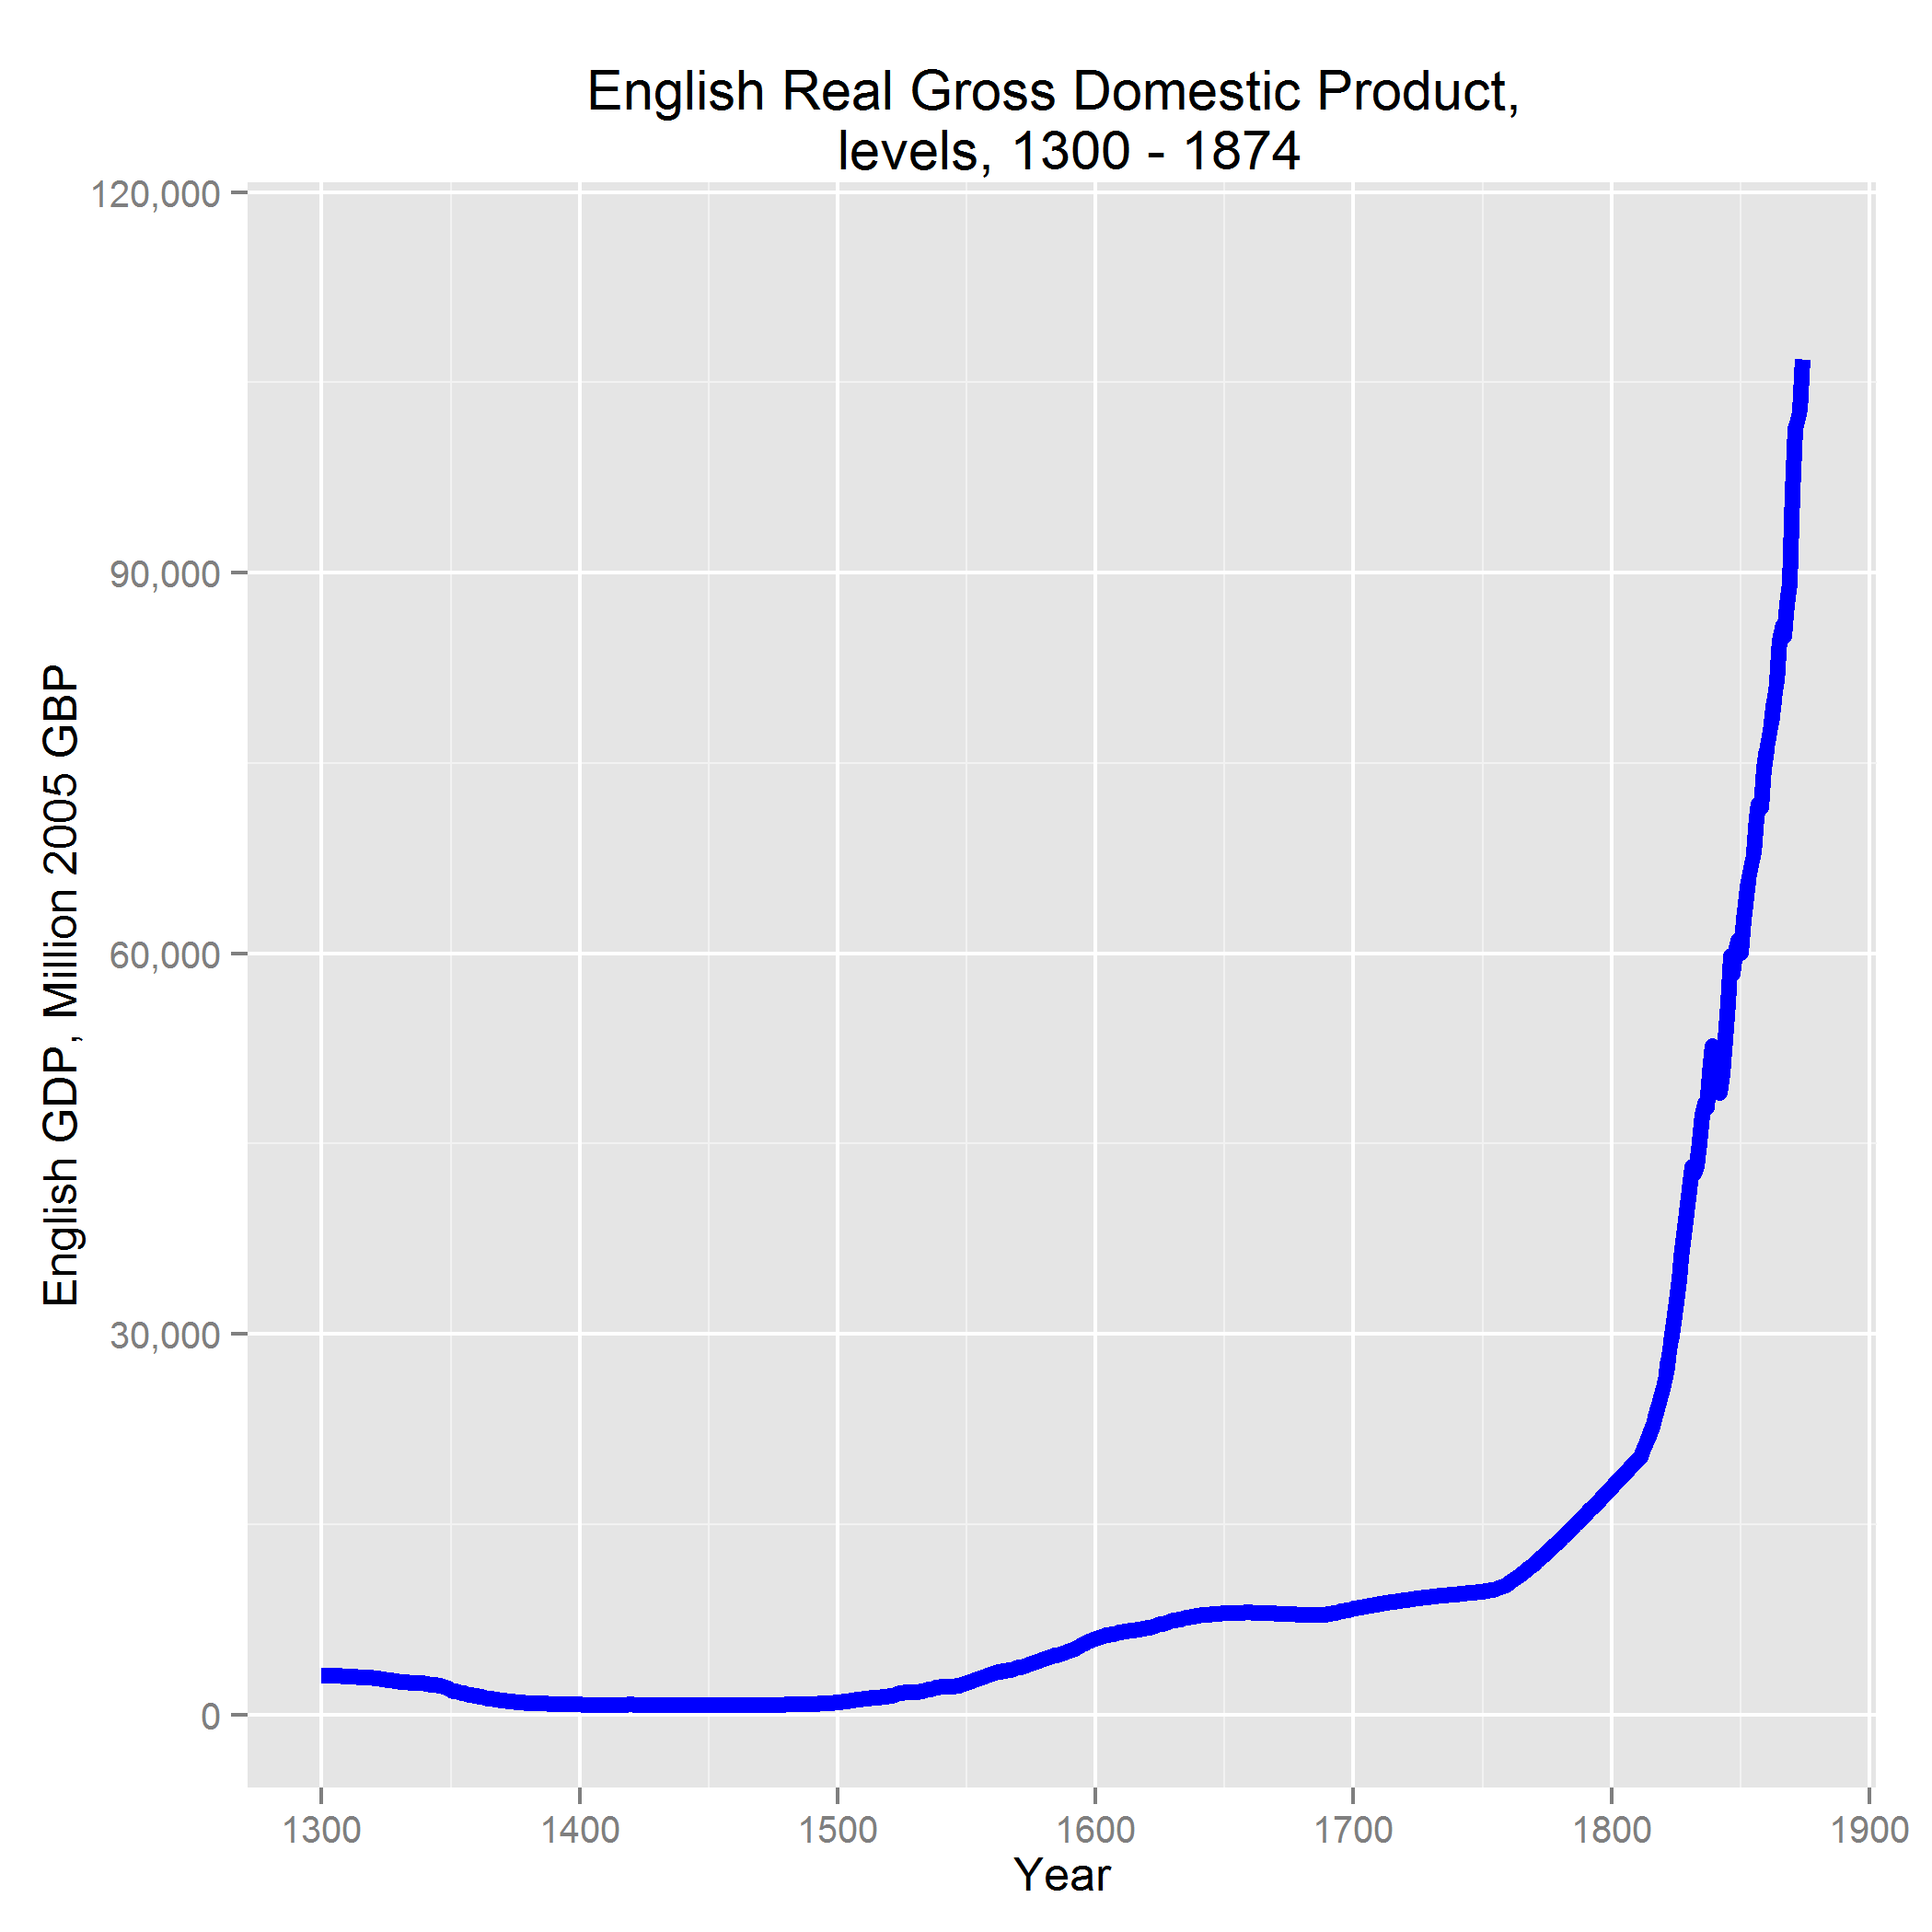
\includegraphics[width=0.39\textwidth]{ggdp}}
		\mbox{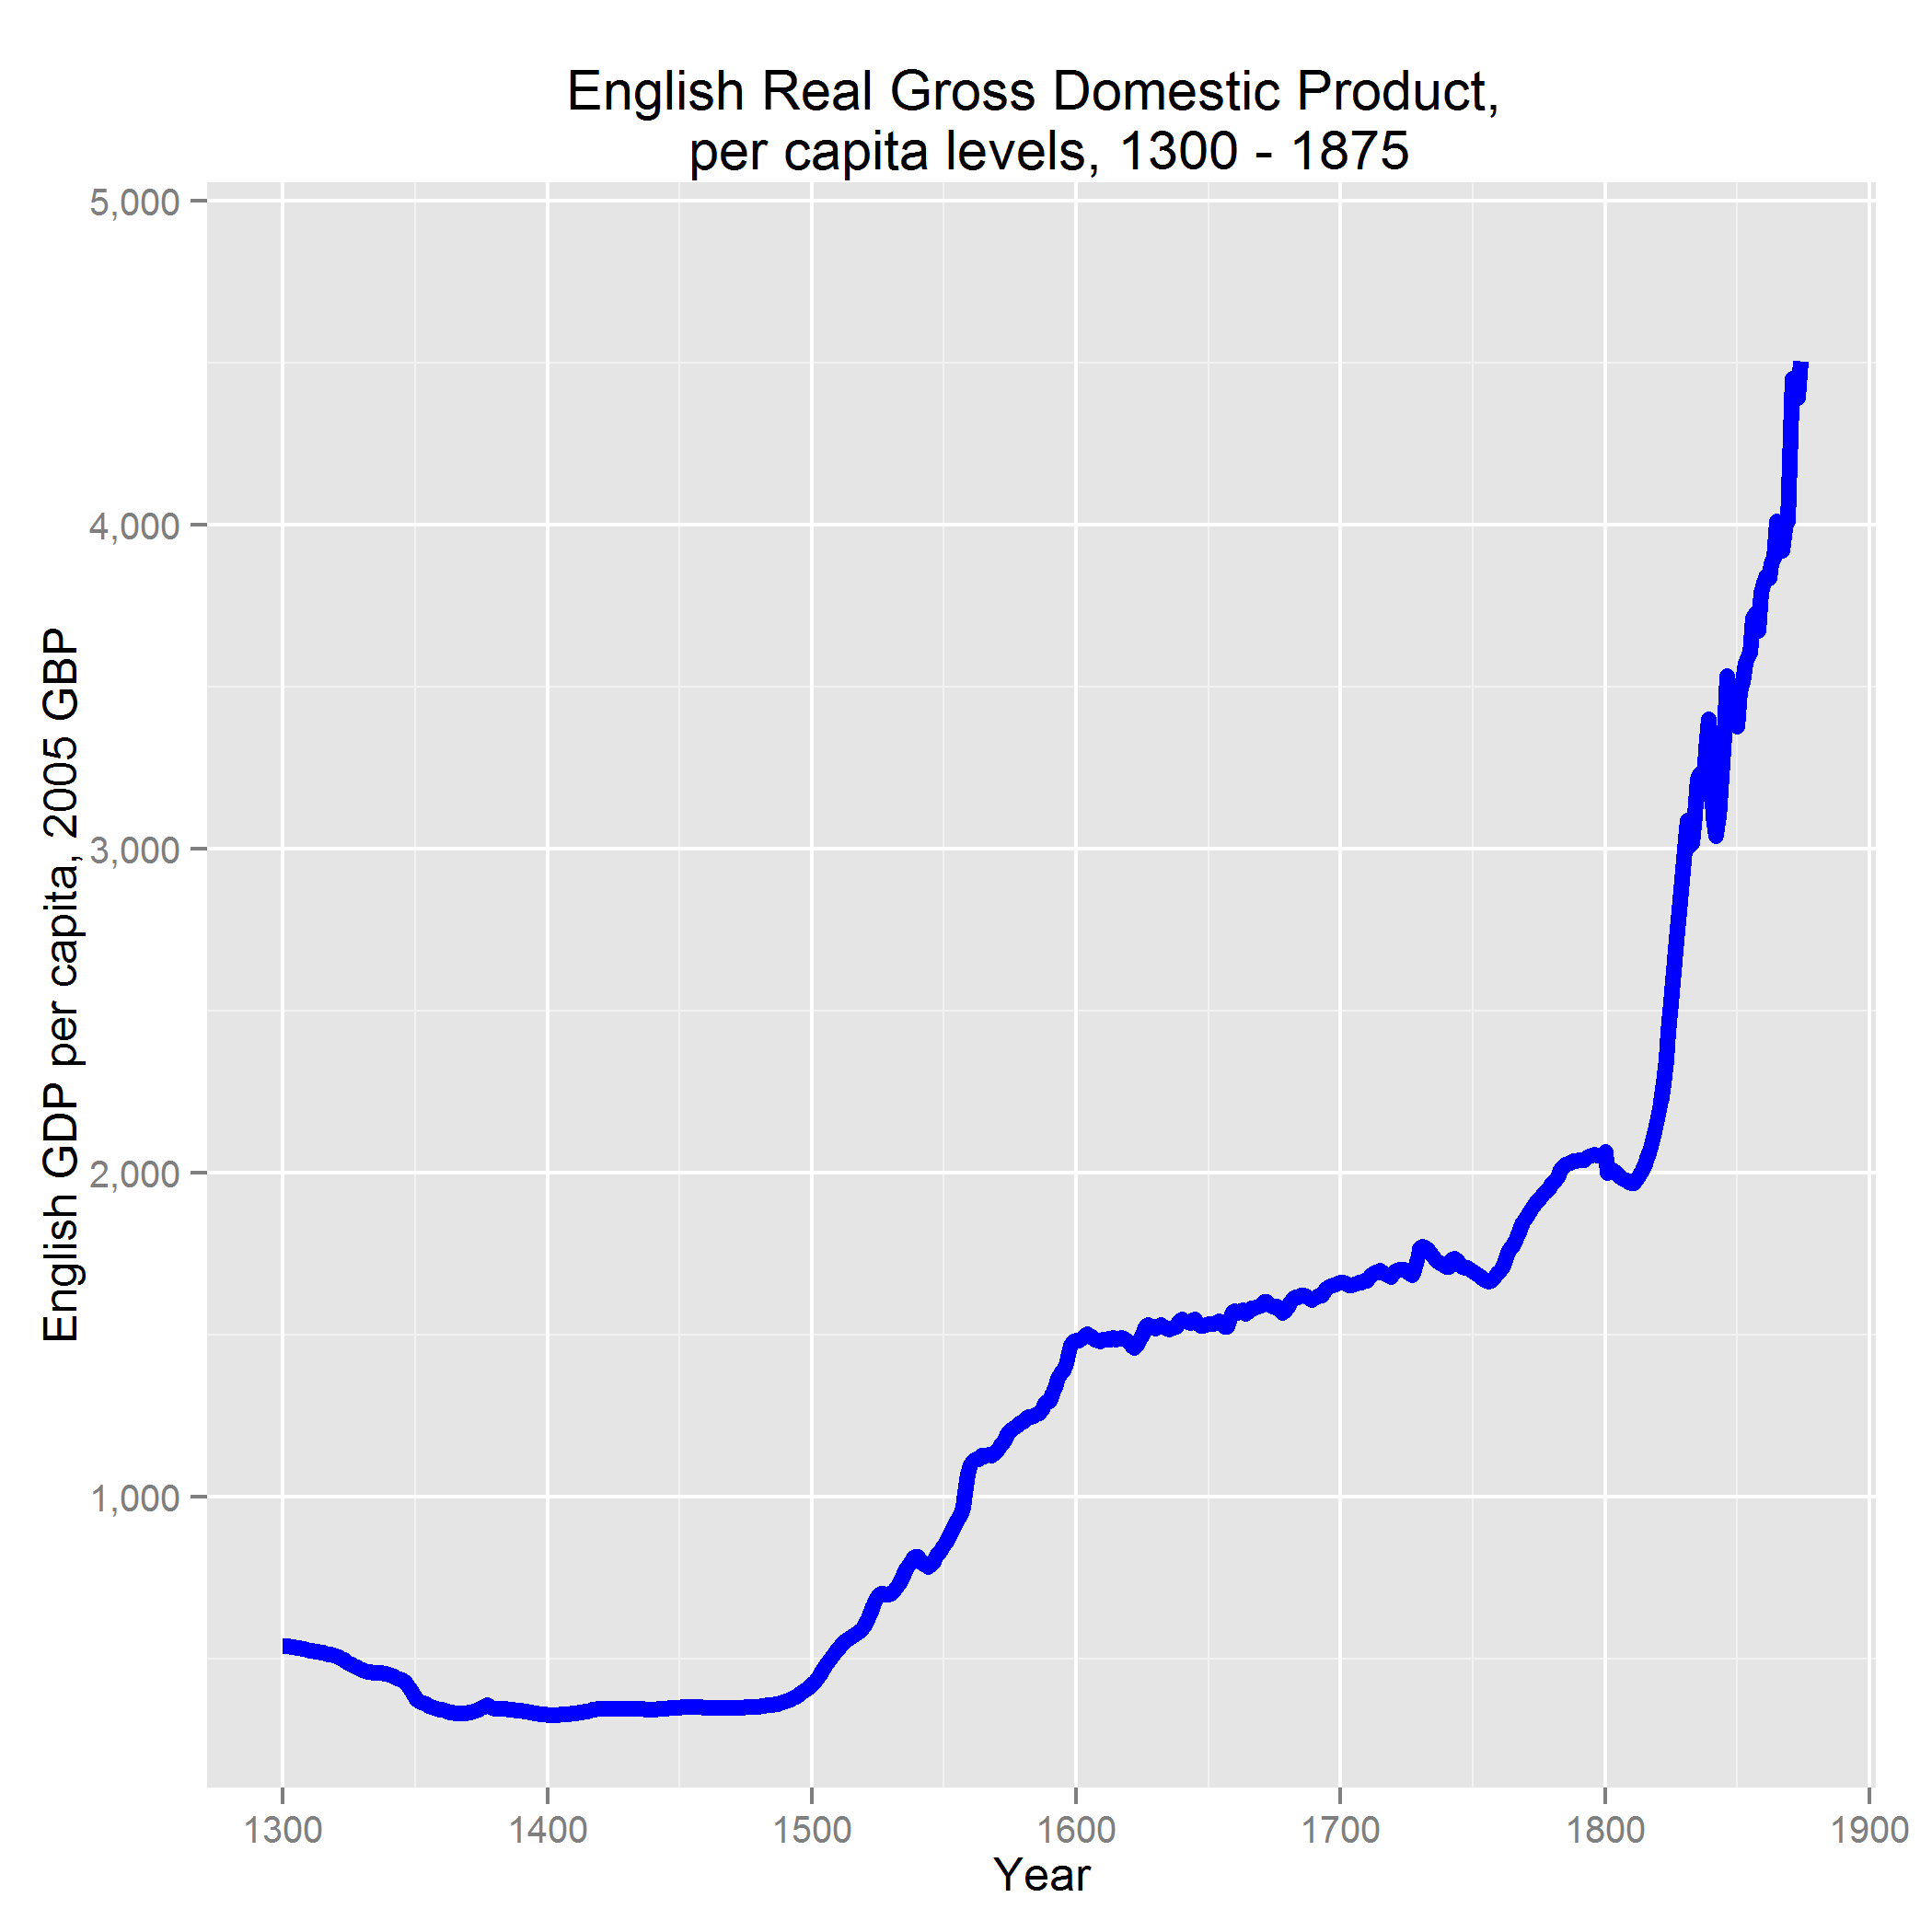
\includegraphics[width=0.39\textwidth]{ggdppop}}
		\mbox{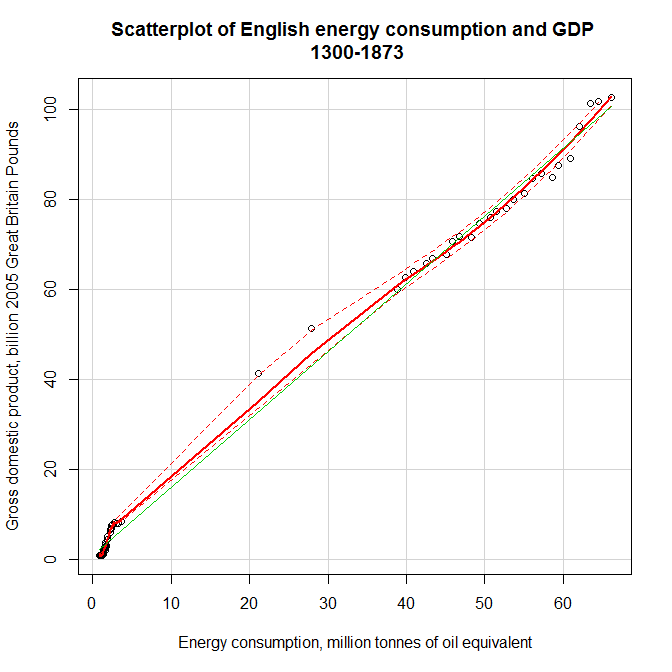
\includegraphics[width=0.39\textwidth]{scatterplot.png}}
		}
\end{figure} \vspace*{-0.4in}
Two energy consumption revolutions driving the machine-age, productivity gains, and rising living standards; no ``Solow'' residual required. This is arguably the deepest, physical (real), identity in all of economic theory
\end{frame}

\begin{frame}
\frametitle{Comparative energy consumption}
\begin{table}[htb]
	\centering
	\begin{tabular}{lrrrr}
	\hline
	Year&England&China&Netherlands&India\\
	\hline \hline
	1650$^a$&&&0.63&  \\
	1820&0.61&&&\\
	1840$^a$ &&&0.33& \\
	1870&2.21&\\
	1970$^a$ &&&8.07&0.33 \\
	1973&&0.48&&\\
	1998$^b$&6.56&1.18\\
	2008$^b$&5.99&2.56&9.86&  \\
	\hline
	\end{tabular}
	\caption{Per-Capita Primary Energy Consumption,	annual Tonnes of Oil Equivalent. \textit{Source:} Angus Maddison, $^a$de Zeeuw, $^b$US DOE EIA}
	\label{tab:maddison_energy}
	\end{table}
\end{frame}	

\begin{frame}
\frametitle{Microeconomic theory $\Rightarrow$ economics is a sufficient IR explanation: toward a theory of energy substitution} 
\pause
%\scriptsize{
\small{
%		\pause		
		\begin{equation}
		\label{eq:mrp}
		\frac{\text{Marginal Product}_{\text{wood Joule}}}{\text{Price}_{\text{wood Joule}}} \ll \frac{\text{Marginal Product}_{\text{coal Joule}}}{\text{Price}_{\text{coal Joule}}}
		\end{equation}
		\pause \vspace*{-0.2in}
		\center First energy revolution: China 900 -- 1200 (Northern Sung)\pause;\\ England 1590 -- 1700
		\pause \vspace*{0.2in}
		\begin{equation}
		\label{eq:mrp2}
		\frac{\text{Marginal Product}_{\text{labor Joule}}}{\text{Price}_{\text{labor Joule}}} \ll \frac{\text{Marginal Product}_{\text{steam Joule}}}{\text{Price}_{\text{steam Joule}}}
		\end{equation}
		\pause \vspace*{-0.2in}
		\begin{center} 
		Second energy revolution: England 1700 -- 1873\pause,\\ but not in China\\
		\pause \vspace*{0.2in}
		The RHS of (2) was so large, it induced a major positive aggregate supply shock \pause and large income effects
		\end{center}
}
\end{frame}


\begin{frame}
\frametitle{Relevant price ratios induce behavioral changes $\Rightarrow$ induced innovation} %\textit{Source:} Robert Allen (2009)}
\begin{figure}[p!]
%\center
%\caption{Real wage to energy ratios\\\textit{Source:} Robert Allen (2009)}
\label{fig:wage-energy}
		\caption{Sources (l to r) Nef, Allen, Allen}
		\centerline{
		\mbox{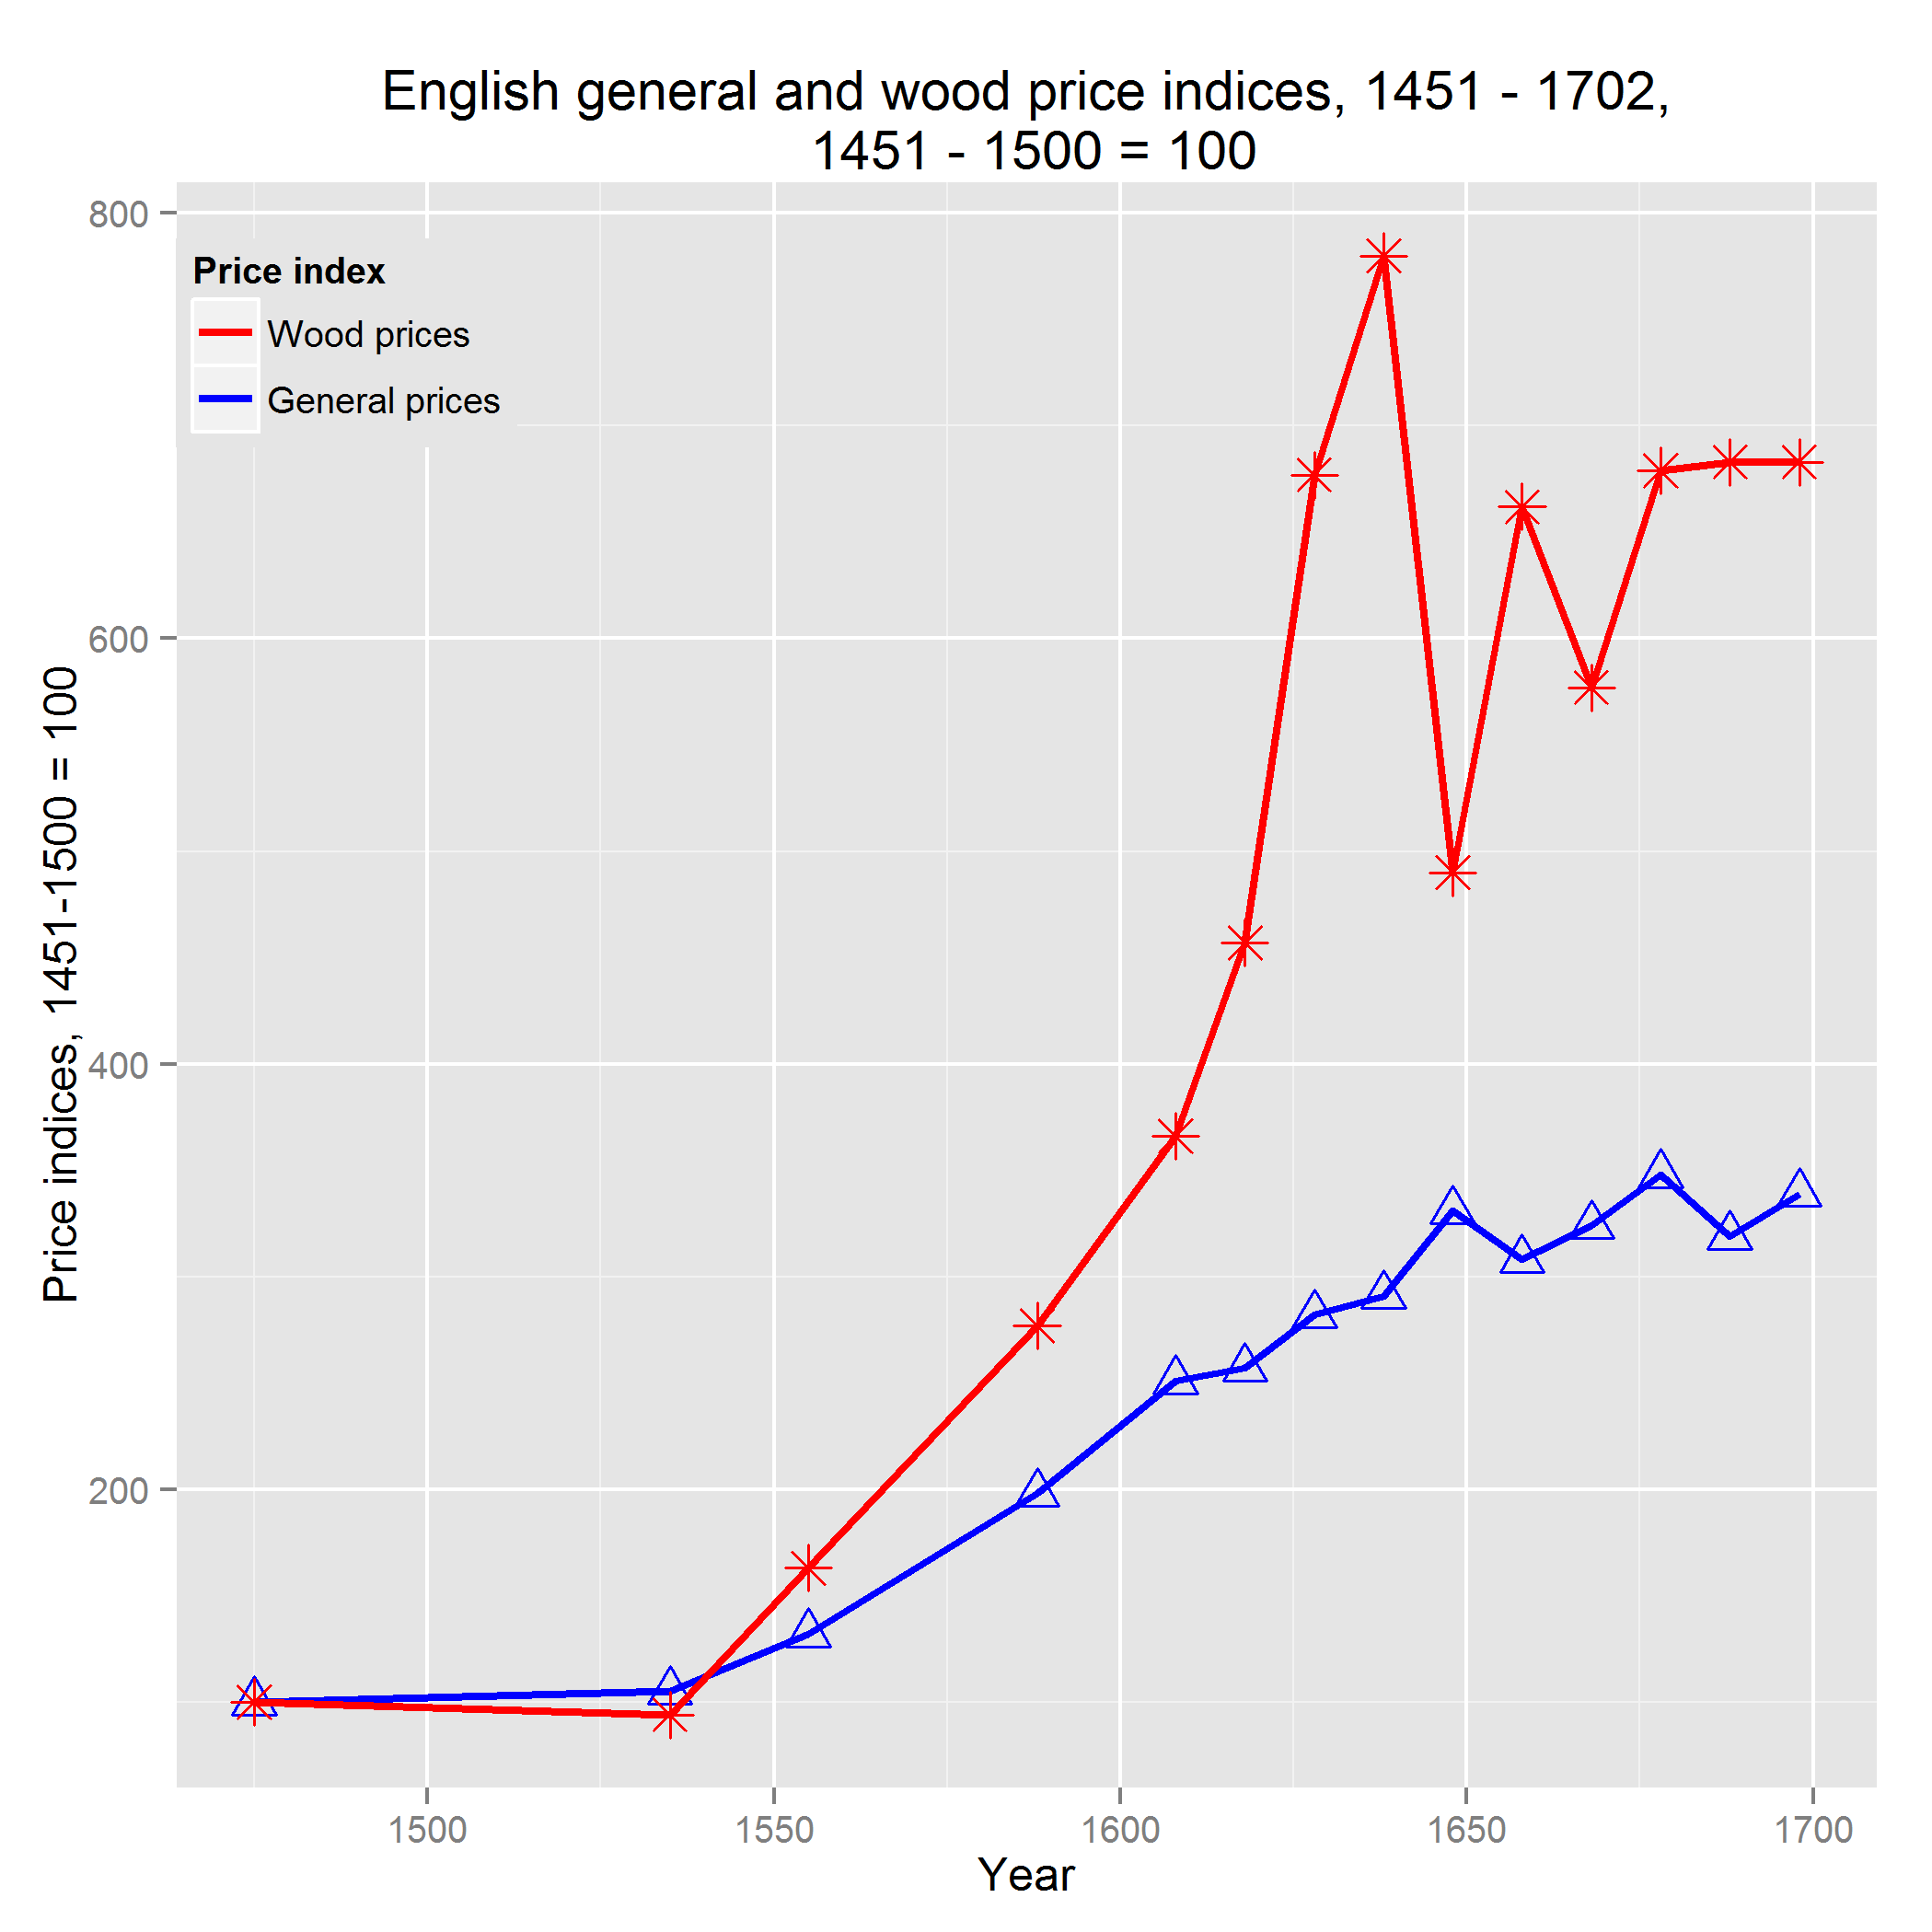
\includegraphics[width=0.39\textwidth]{woodPrice}}
		\mbox{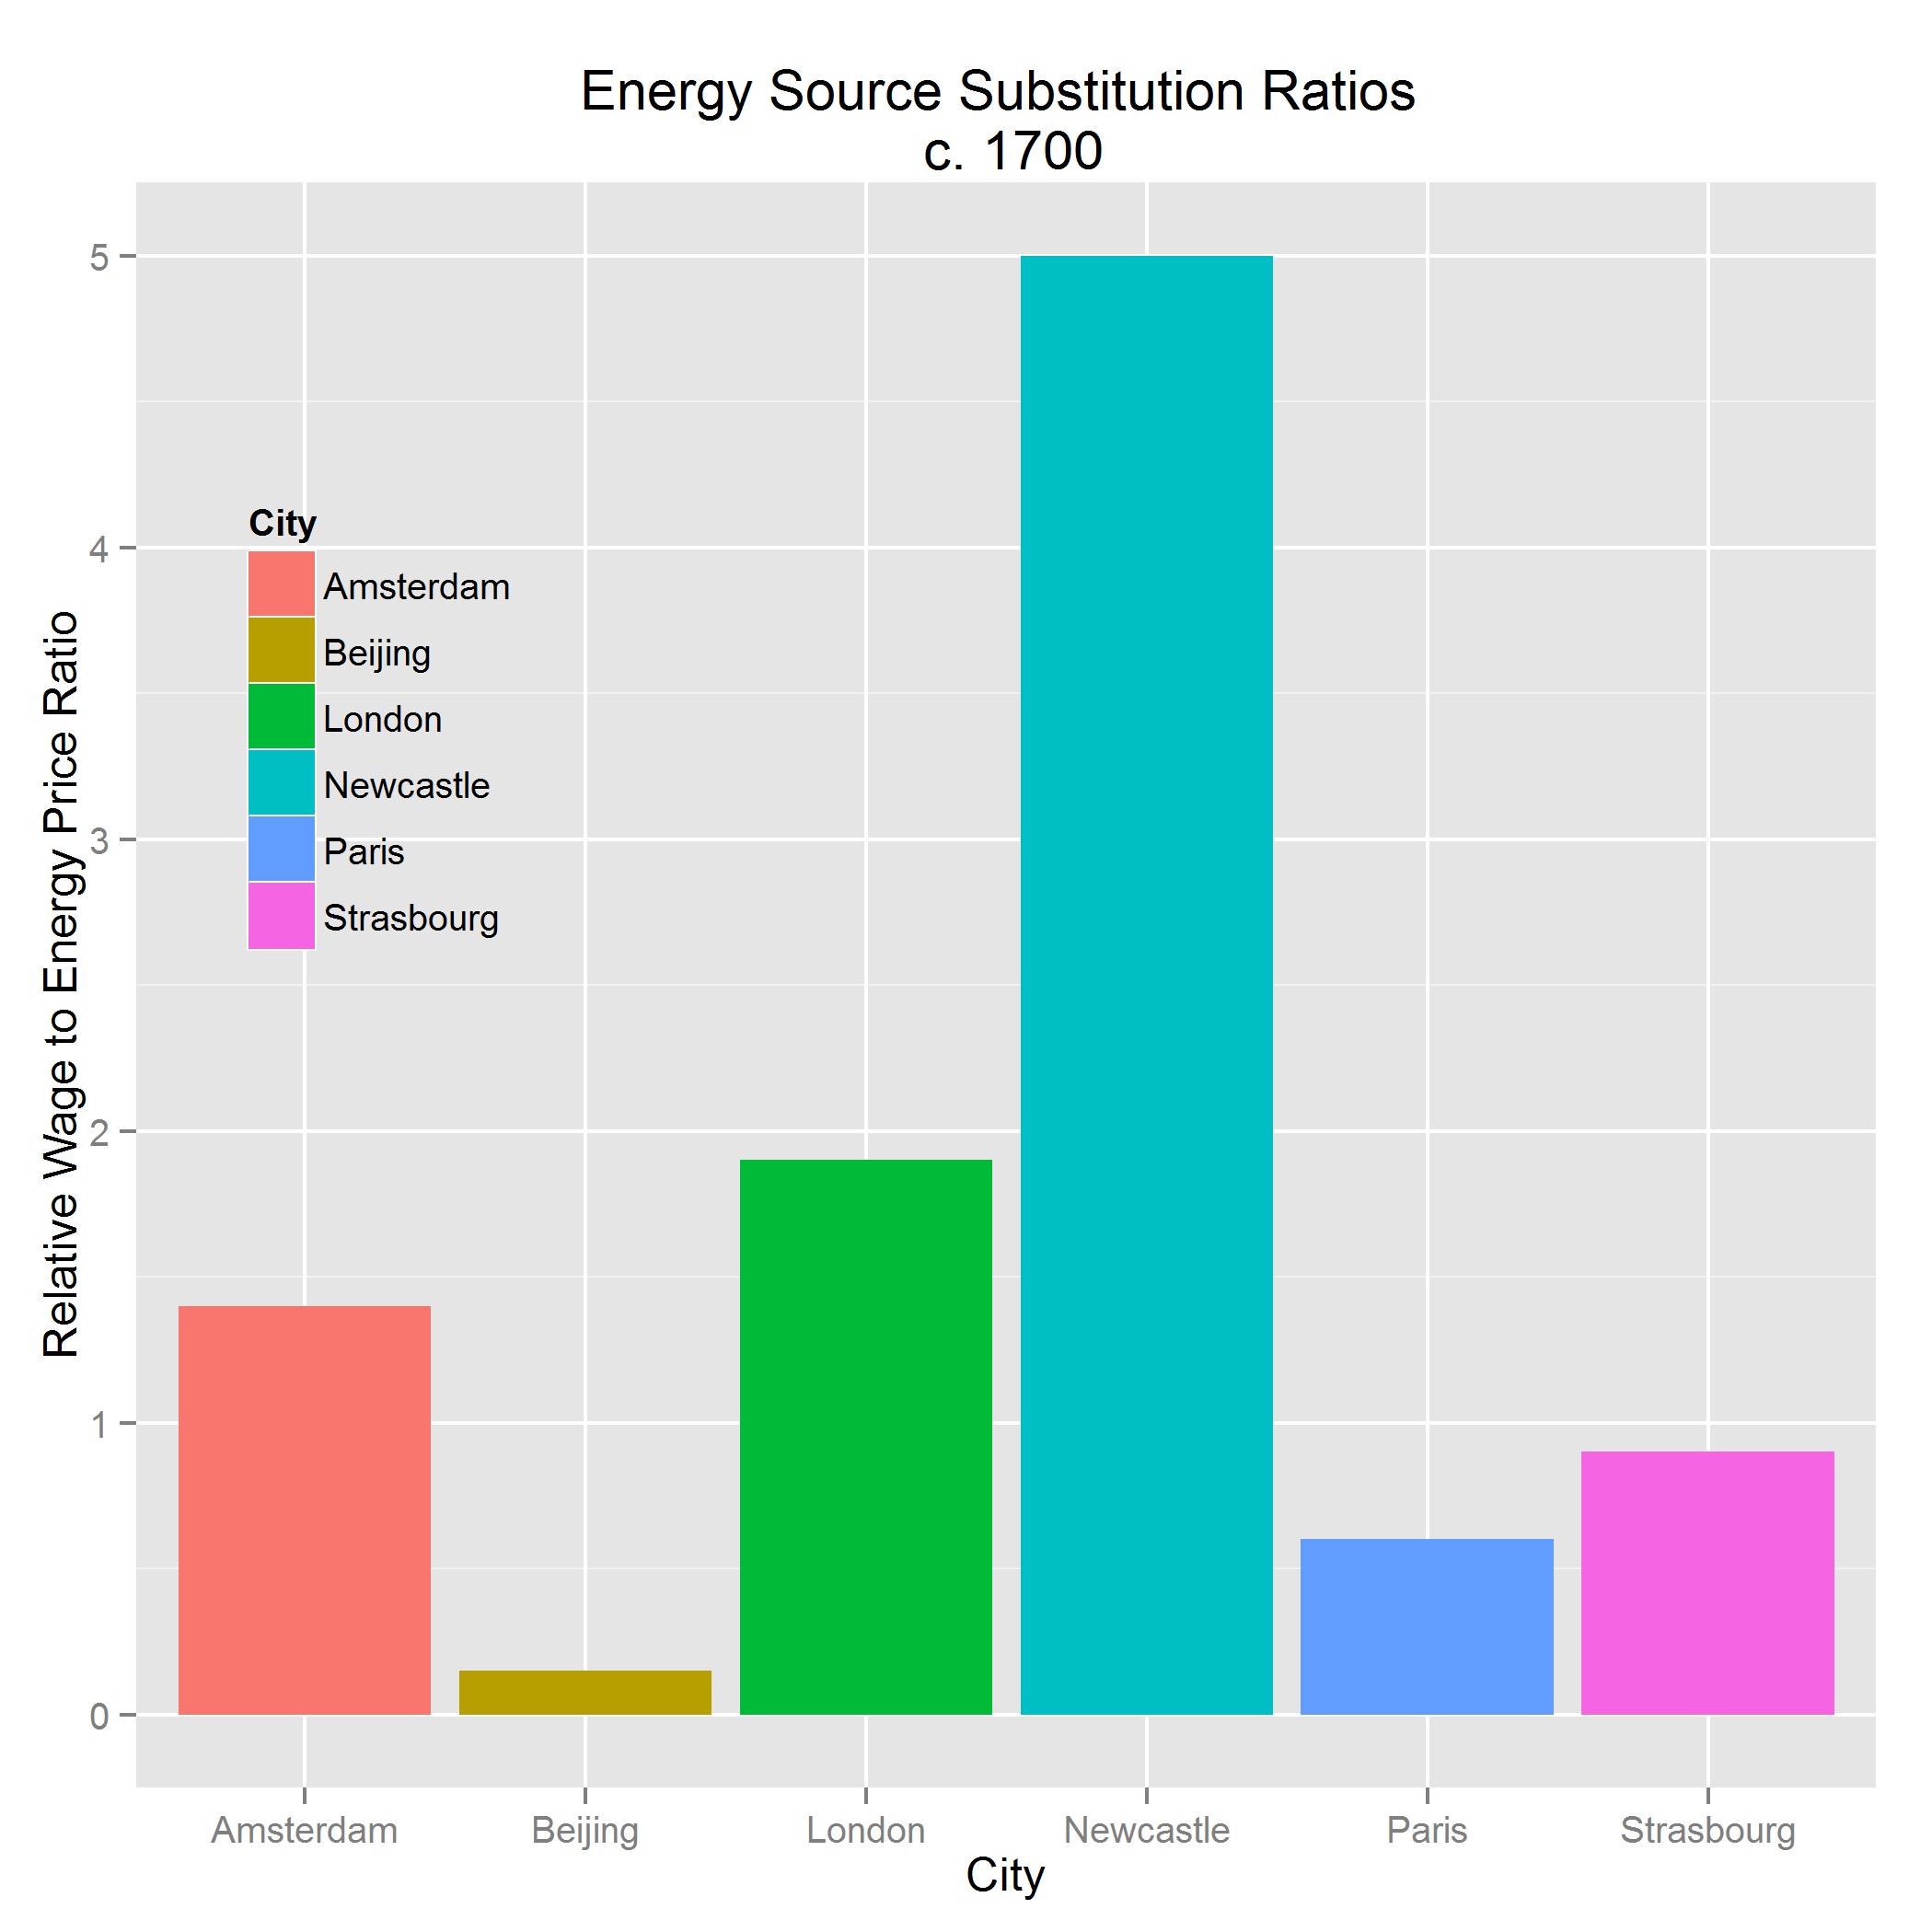
\includegraphics[width=0.39\textwidth]{wage-energy}}
		\mbox{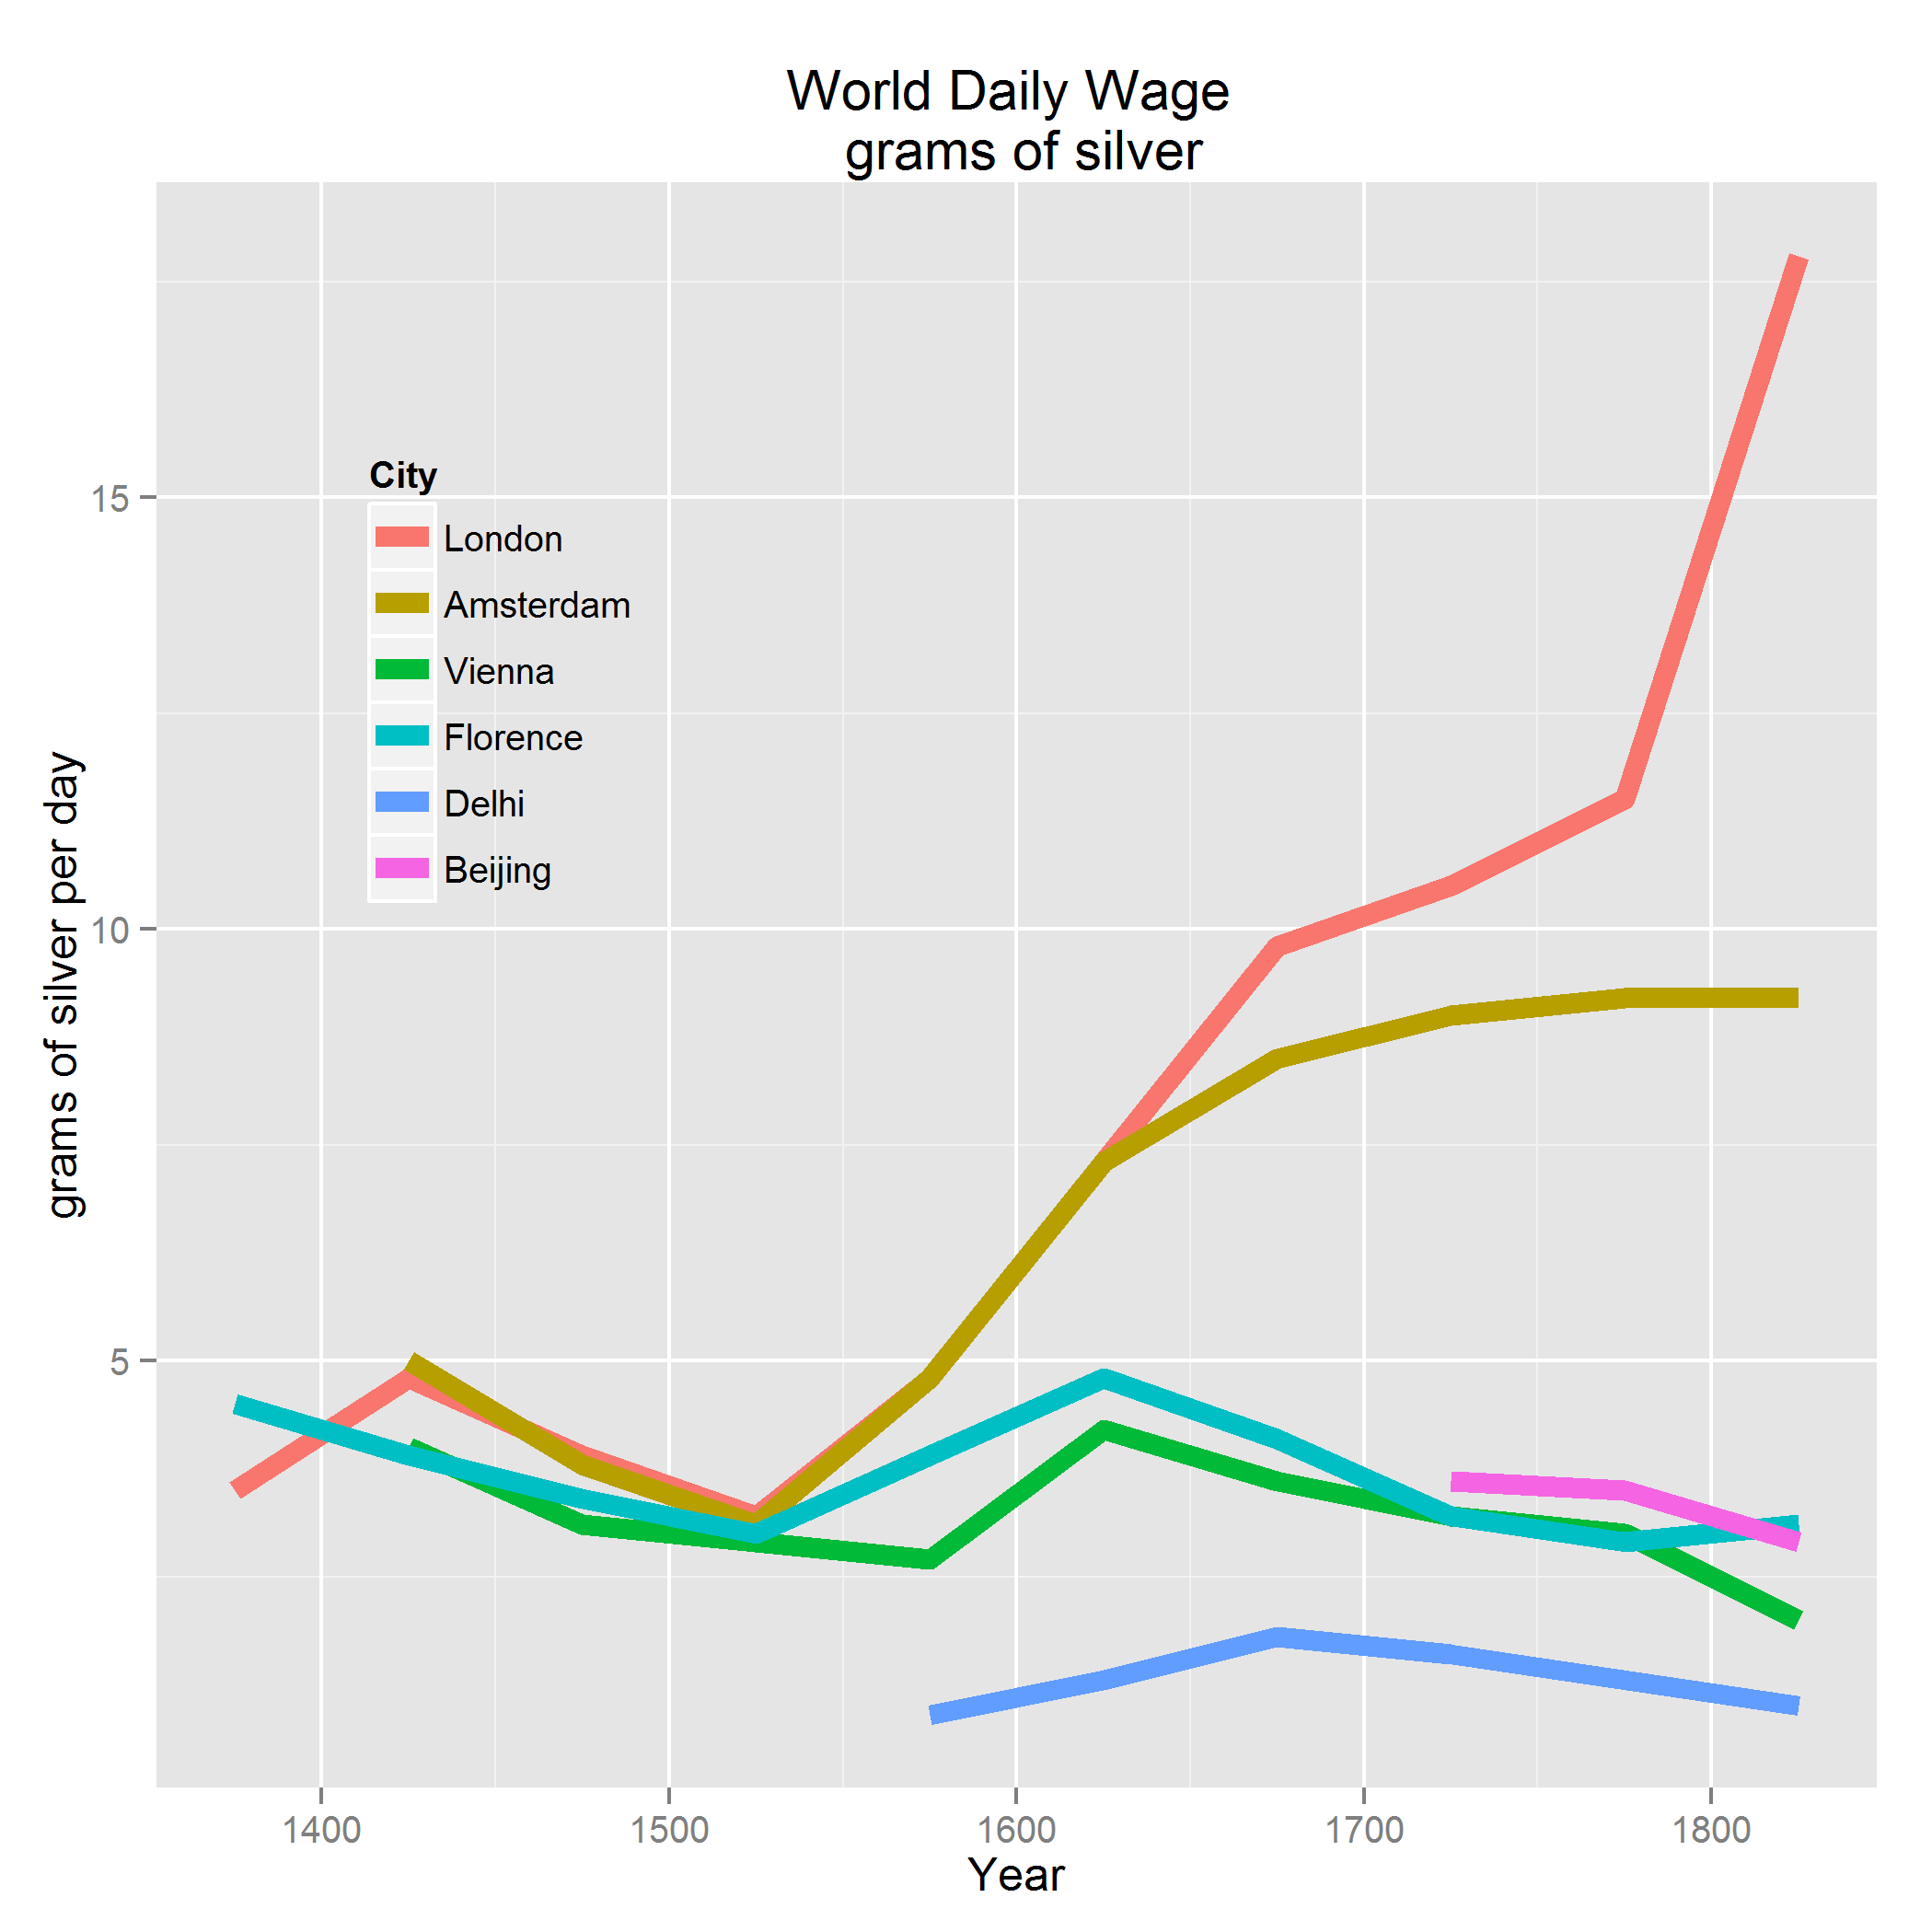
\includegraphics[width=0.39\textwidth]{gworldwages}}
		}
\end{figure}
\end{frame}

\begin{frame}
\frametitle{What about institutions?}
\begin{itemize}
\item Historical materialism \pause $\Rightarrow$ induced institutions\pause
\item Is the juice worth the squeeze? \pause 
	\begin{itemize}
	\item Why property rights if no property? \pause 
	\item Why a Bank of England if no borrowers? \pause 
	\end{itemize}
\item Especially, why Industrial Capitalism if no significant machines and capital is not required to chop down trees?
\end{itemize}
\end{frame}

\begin{frame}
\frametitle{Chinese institutional revisionism $\Rightarrow$ sufficient institutions}
\begin{itemize}
\footnotesize{
\item Huang, Philip C. 1990. The Peasant Family and Rural Development in the Yangzi Delta, 1350-1988
\item Wong, R. Bin. 1997. China Transformed: Historical Change and the Limits of European Experience
\item Lee, James Z., and Cameron D. Campbell. 1997. Fate and Fortune in Rural China : Social Organization and Population Behavior in Liaoning, 1774-1873
\item Li, Bozhong. 1998. Agricultural Development in Jiangnan, 1620-1850
\item Pomeranz, Kenneth. 2000. The Great Divergence : Europe, China, and the Making of the Modern World Economy
\item Rawski, Thomas G. 1989. Economic Growth in Prewar China. Berkeley: University of California Press.
\item Brandt, Loren. 1989. Commercialization and Agricultural Development: Central and Eastern China 1870-1937. Cambridge: Cambridge University Press.
\item Myers, Ramon H. 1980. The Chinese Economy Past and Present. Belmont, CA: Wadsworth.
\item Xu, Dixin, and Zhengming Wu, eds. Chinese Capitalism, 1522-1840. New York: St. Martin's Press, 2000. 
}
\end{itemize}
\end{frame}

\begin{frame}
\frametitle{No Chinese Industrial Revolution}

	\begin{itemize}
	\item Empirics (even with sparse Chinese data) suggest what happened, and what did not -- no ``second'' energy revolution \pause
	\item Economic theory (micro and macro) explains why \pause
	\item For China, relatively low wages and high energy costs precluded a second energy revolution -- no economic incentive \pause
%	\item Macro- and micro-economics explain a great deal about what happened
	\item Increasingly, scholarship suggests contemporary institutions, and basic technology, were sufficient\pause; thus economics is a compelling primary explanation \pause
	\item Framework applicable across time series, space, and time to inform development scientists
	\item Doesn't this energy story doom us? \pause Yes sort of, and no. More papers coming
	\end{itemize}
\end{frame}

\begin{frame}
\frametitle{Thank you}
\end{frame}

\section{Supplement}


\begin{frame}
\frametitle{Taxonomy of EIR explanations}
\footnotesize{
\begin{table}[p!]
%\caption{Taxonomy of EIR explanations}
\label{tbl:taxonomy}
\begin{tabular}{ll}
Label&Examples\\
\hline \hline
English exceptionalists&Landes (1969), McCloskey (2010), Mokyr (1992,2010)\\
Partial culturalists&Cipolla (1966), Pomeranz (2001), Allen (2009)\\
Primarily energetic&Cottrell (1955), Wrigley (1988,2010), Malanima (2010)\\
Thermodynamicists&Georgescu-Roegen (1975), Ayres (2003), Garrett (2009)\\
\end{tabular}
\end{table}
}
\end{frame}

\begin{frame}
\frametitle{Author/time-span series of energy consumption, GDP, and population}
\begin{figure}[p!]
\center
%\caption{Author/time-span series of energy consumption, GDP, and population}
\label{fig:overall levels}
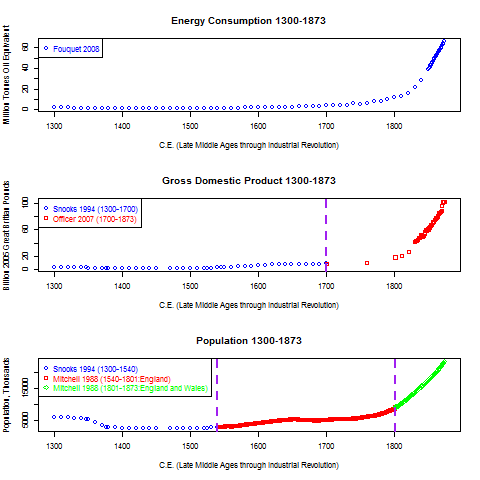
\includegraphics[height=0.8\textheight]{overallLevels}
\end{figure}
\end{frame}

\begin{frame}
		\frametitle{Aggregate Supply - Aggregate Demand \\ Four energy/GDP regimes}
\begin{figure}[p!]
%		\caption{Aggregate Supply - Aggregate Demand \\ Four energy/GDP regimes}
		\label{fig:asad}		
		\centerline{
		\mbox{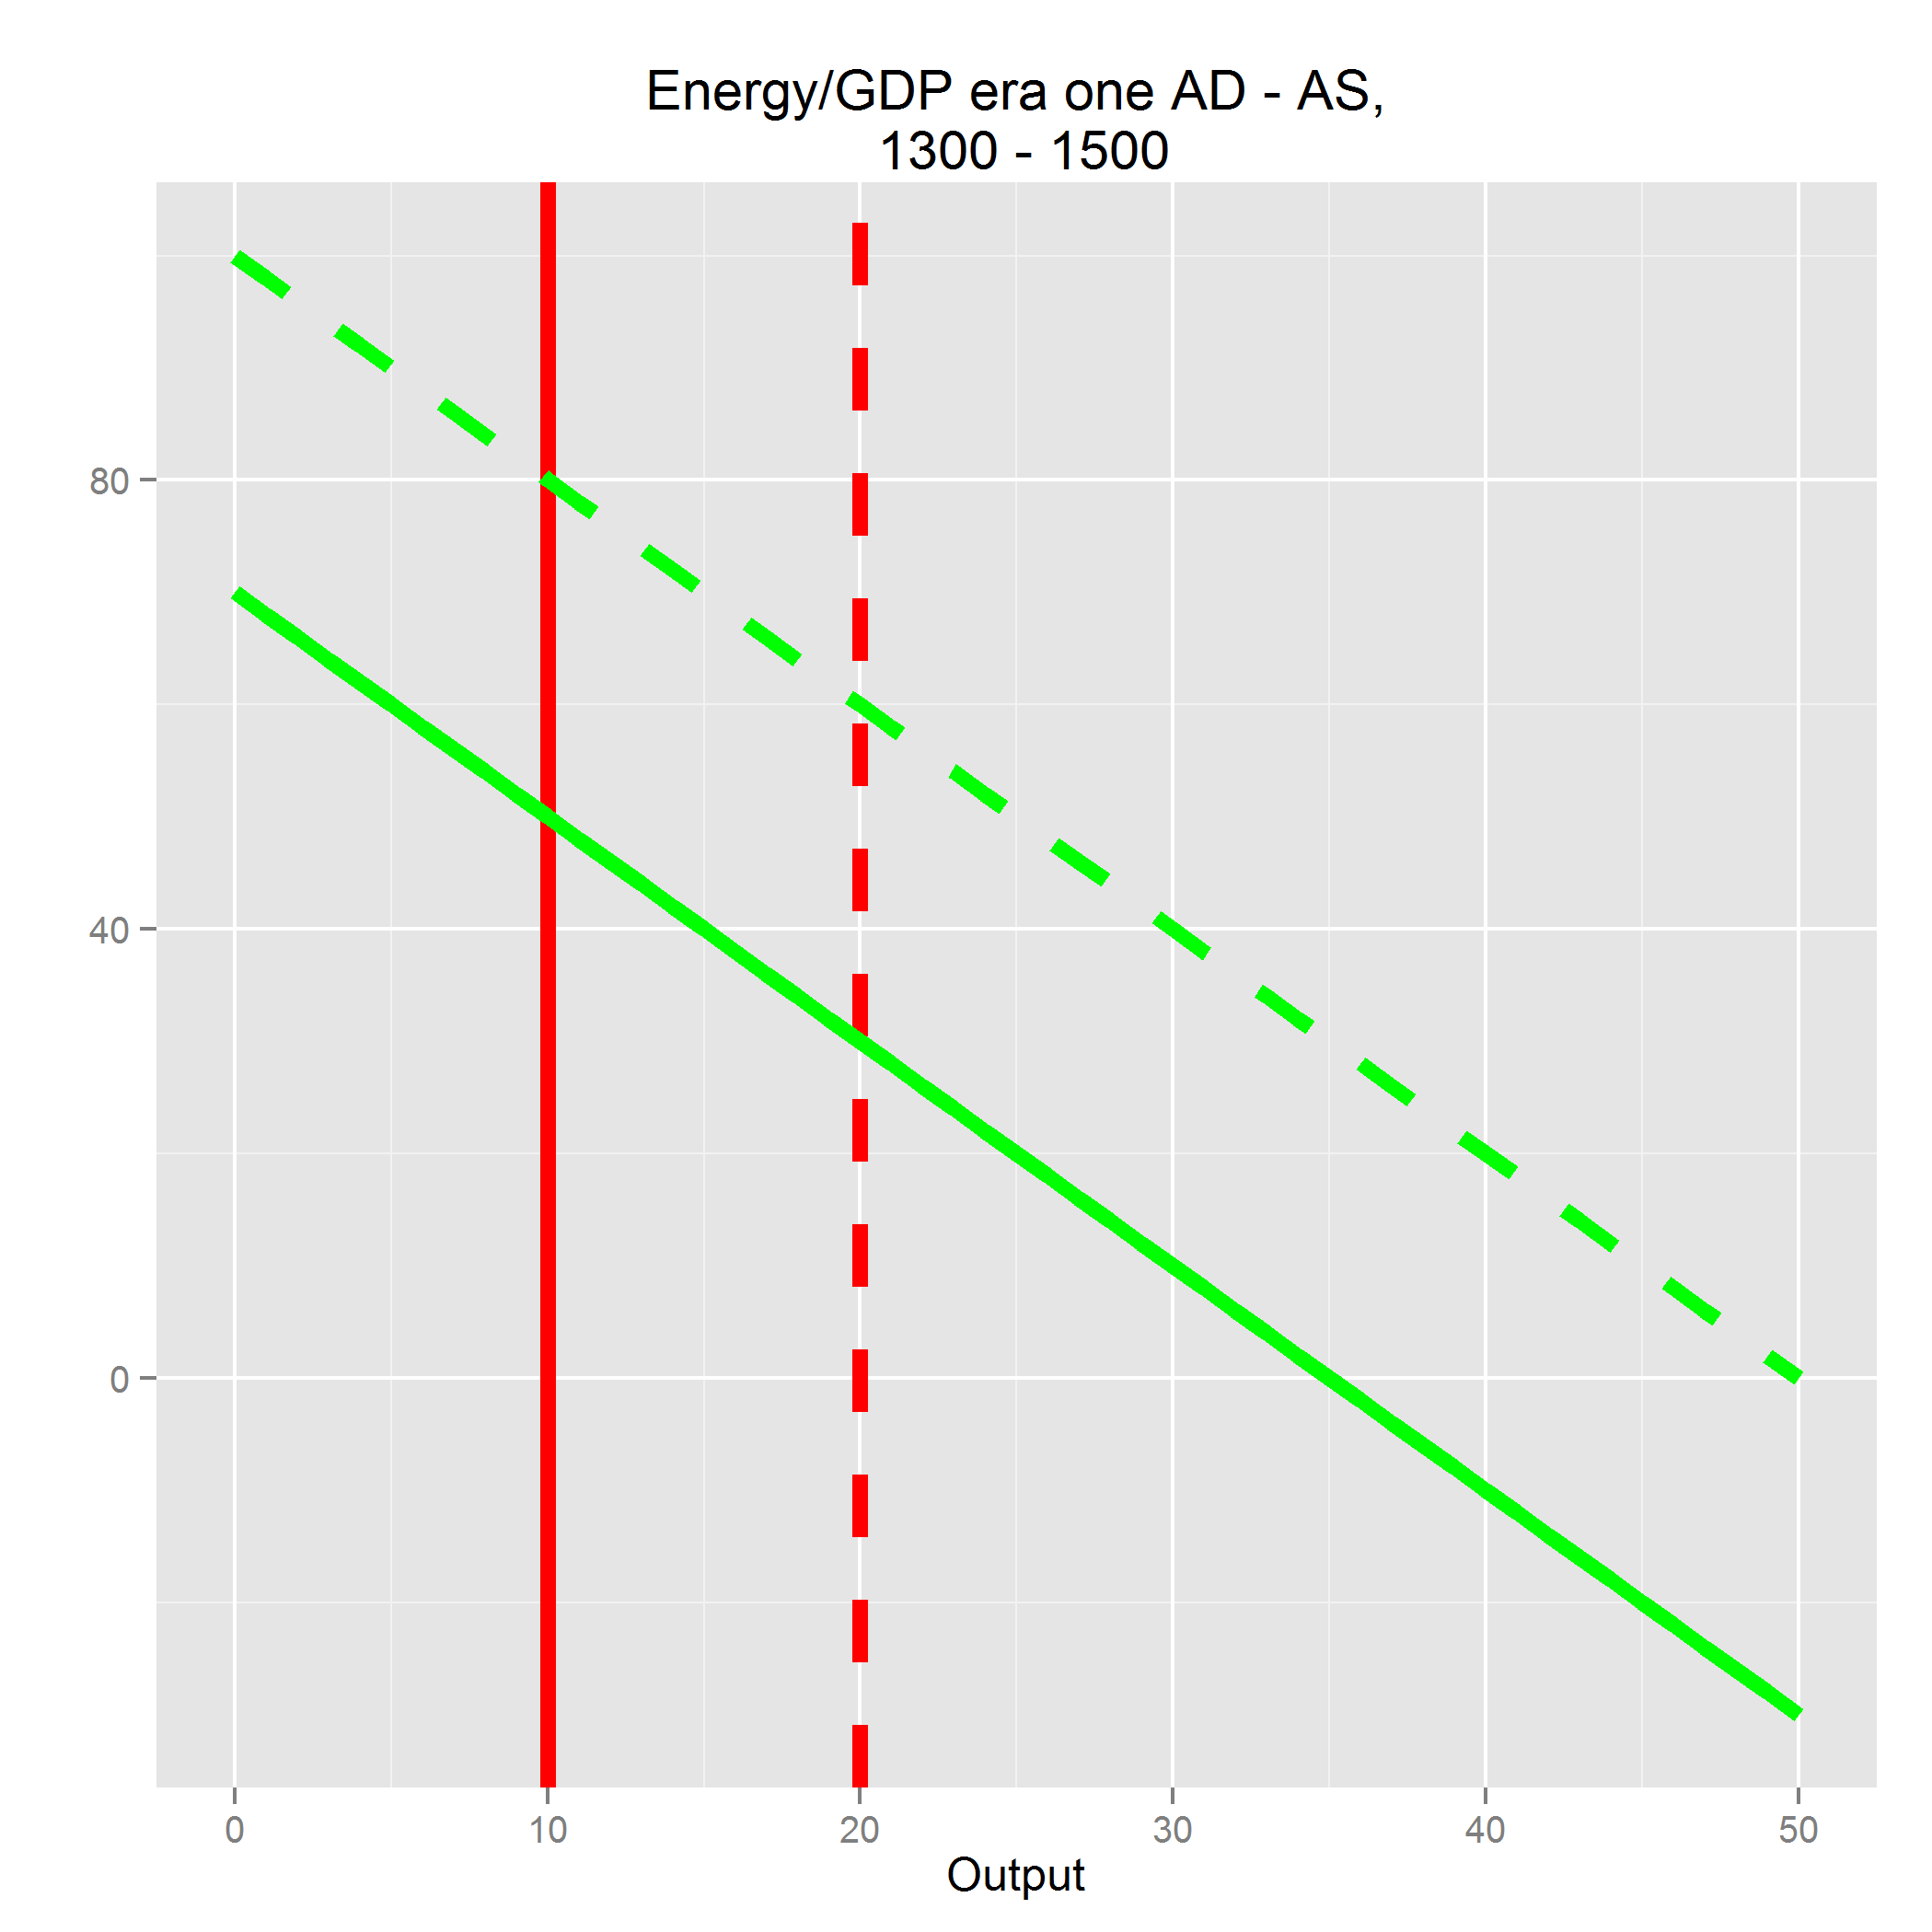
\includegraphics[height=0.35\textheight]{era1}}
		\mbox{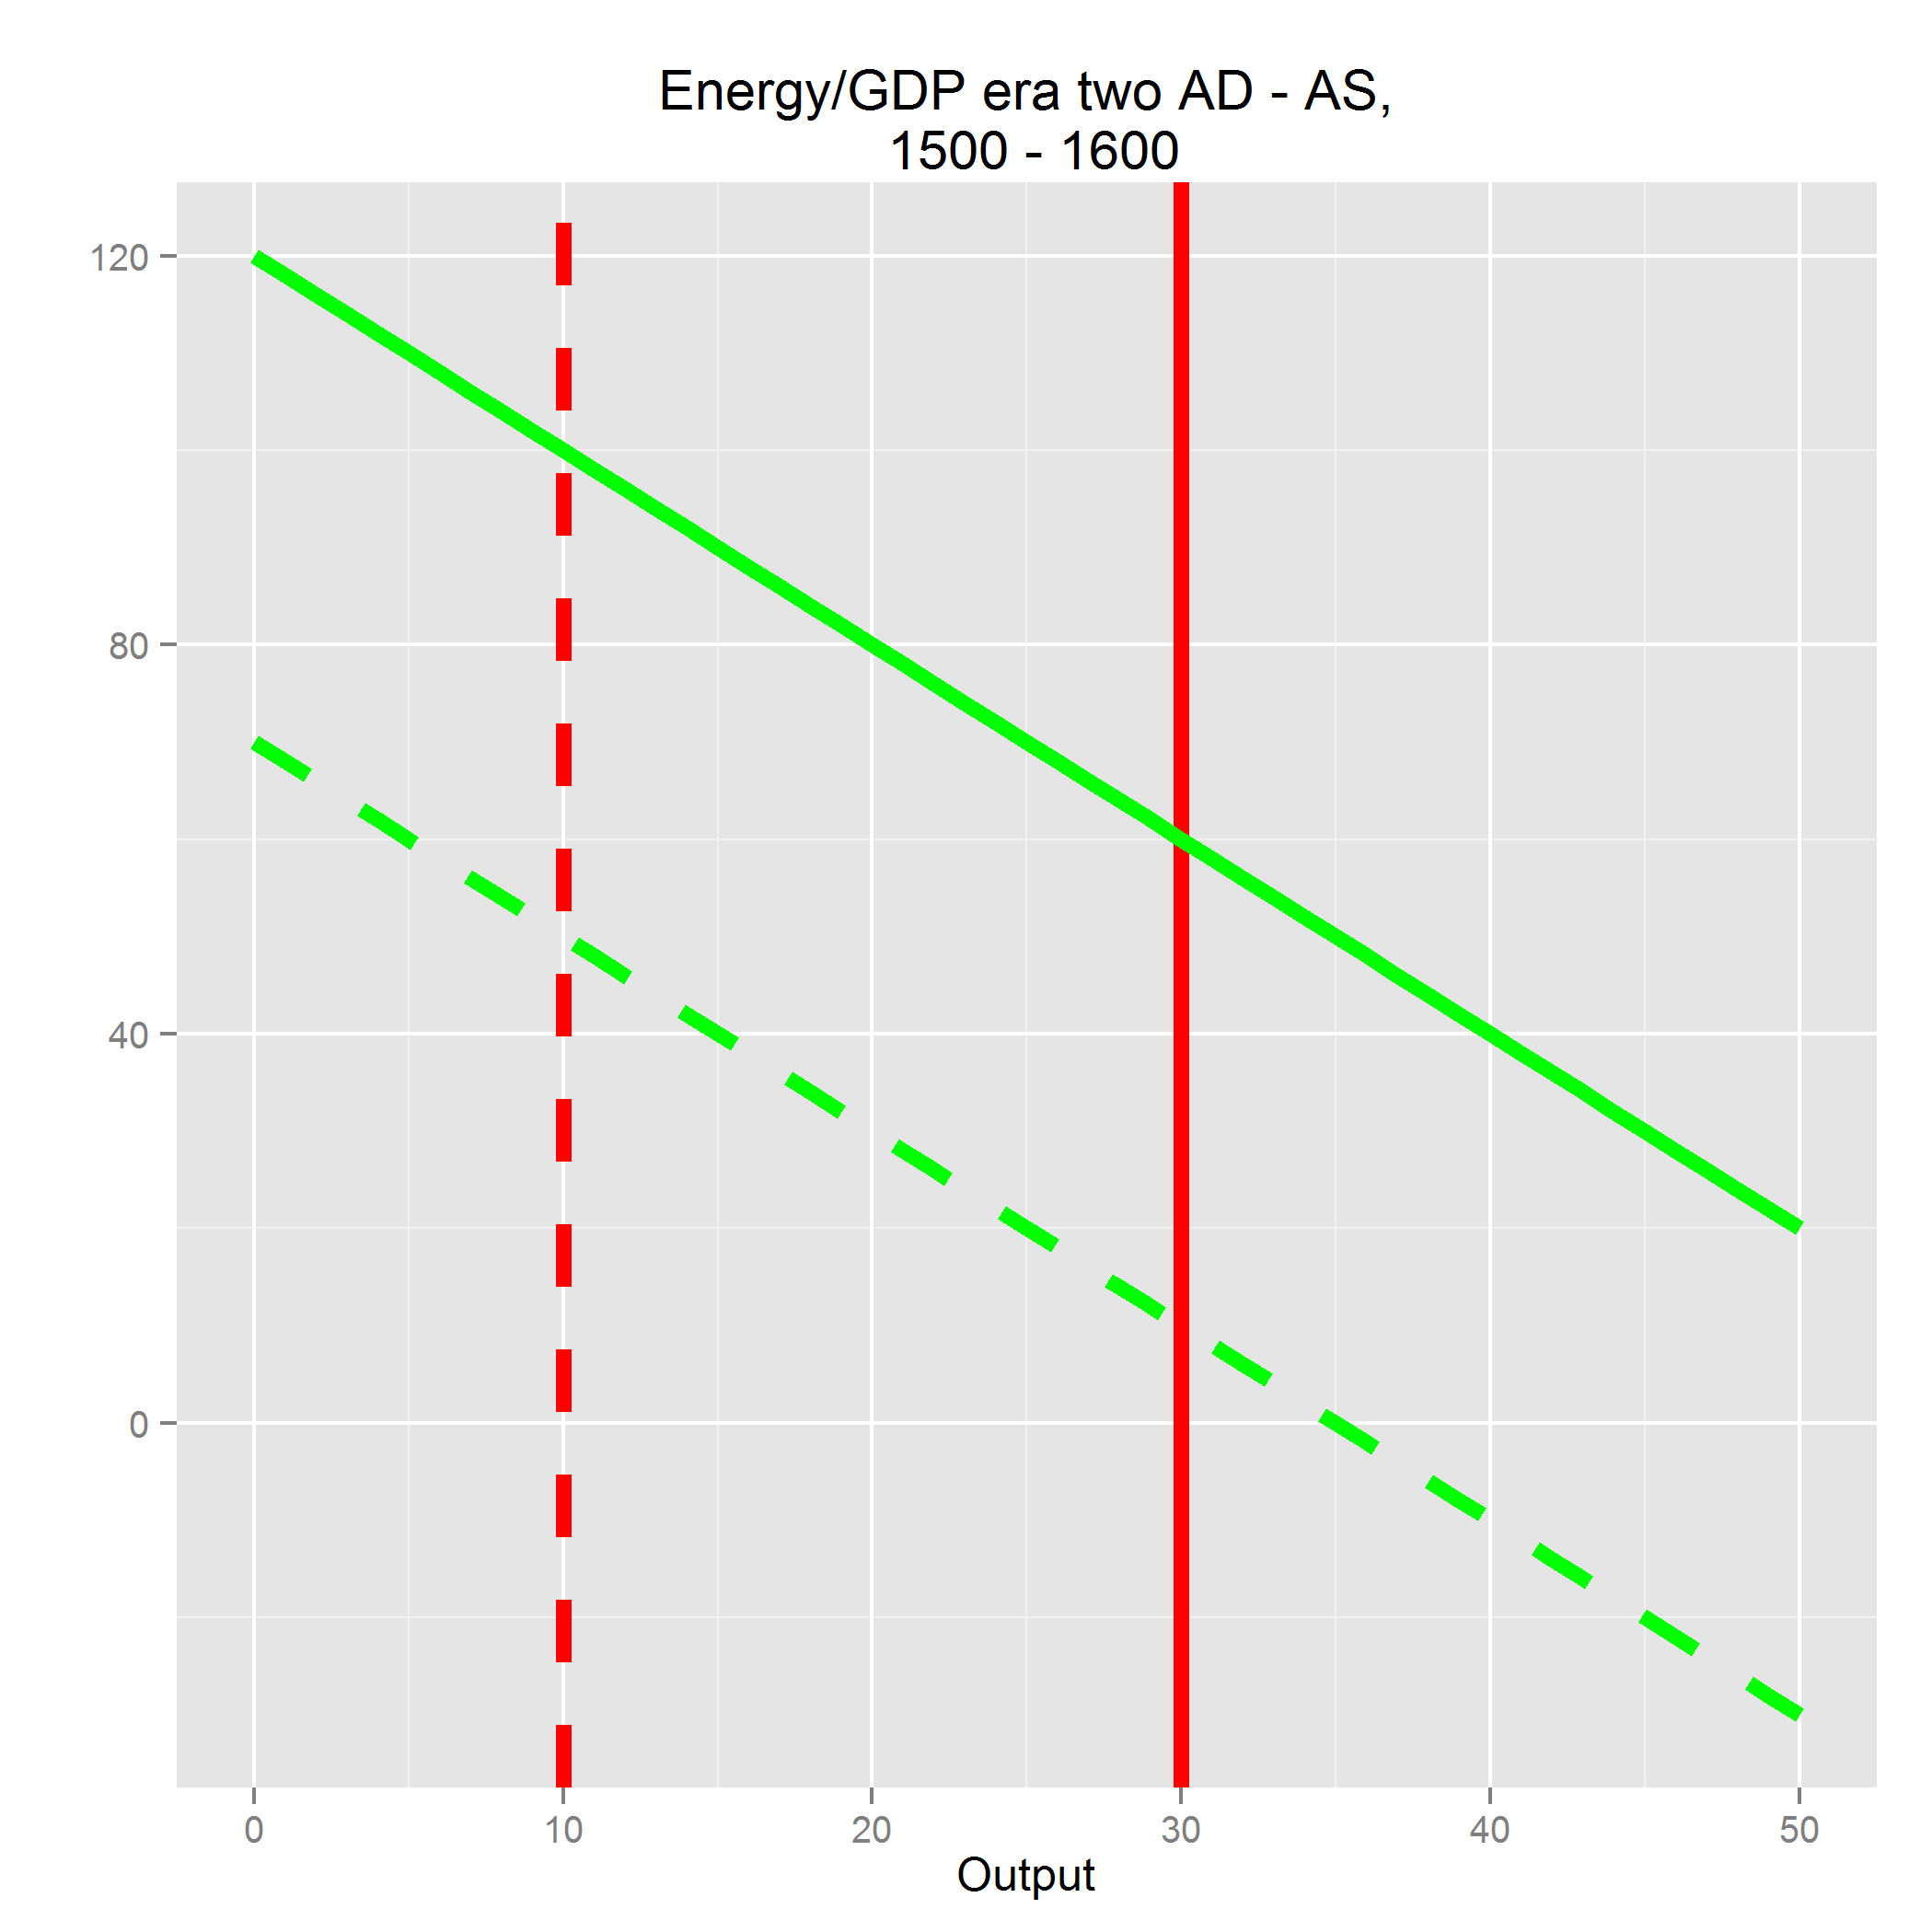
\includegraphics[height=0.35\textheight]{era2}}
		}
		\end{figure}
\begin{figure}[p!]
%		\caption{Aggregate Supply - Aggregate Demand \\ Four energy/GDP regimes}
		\label{fig:asad}		
		\centerline{
		\mbox{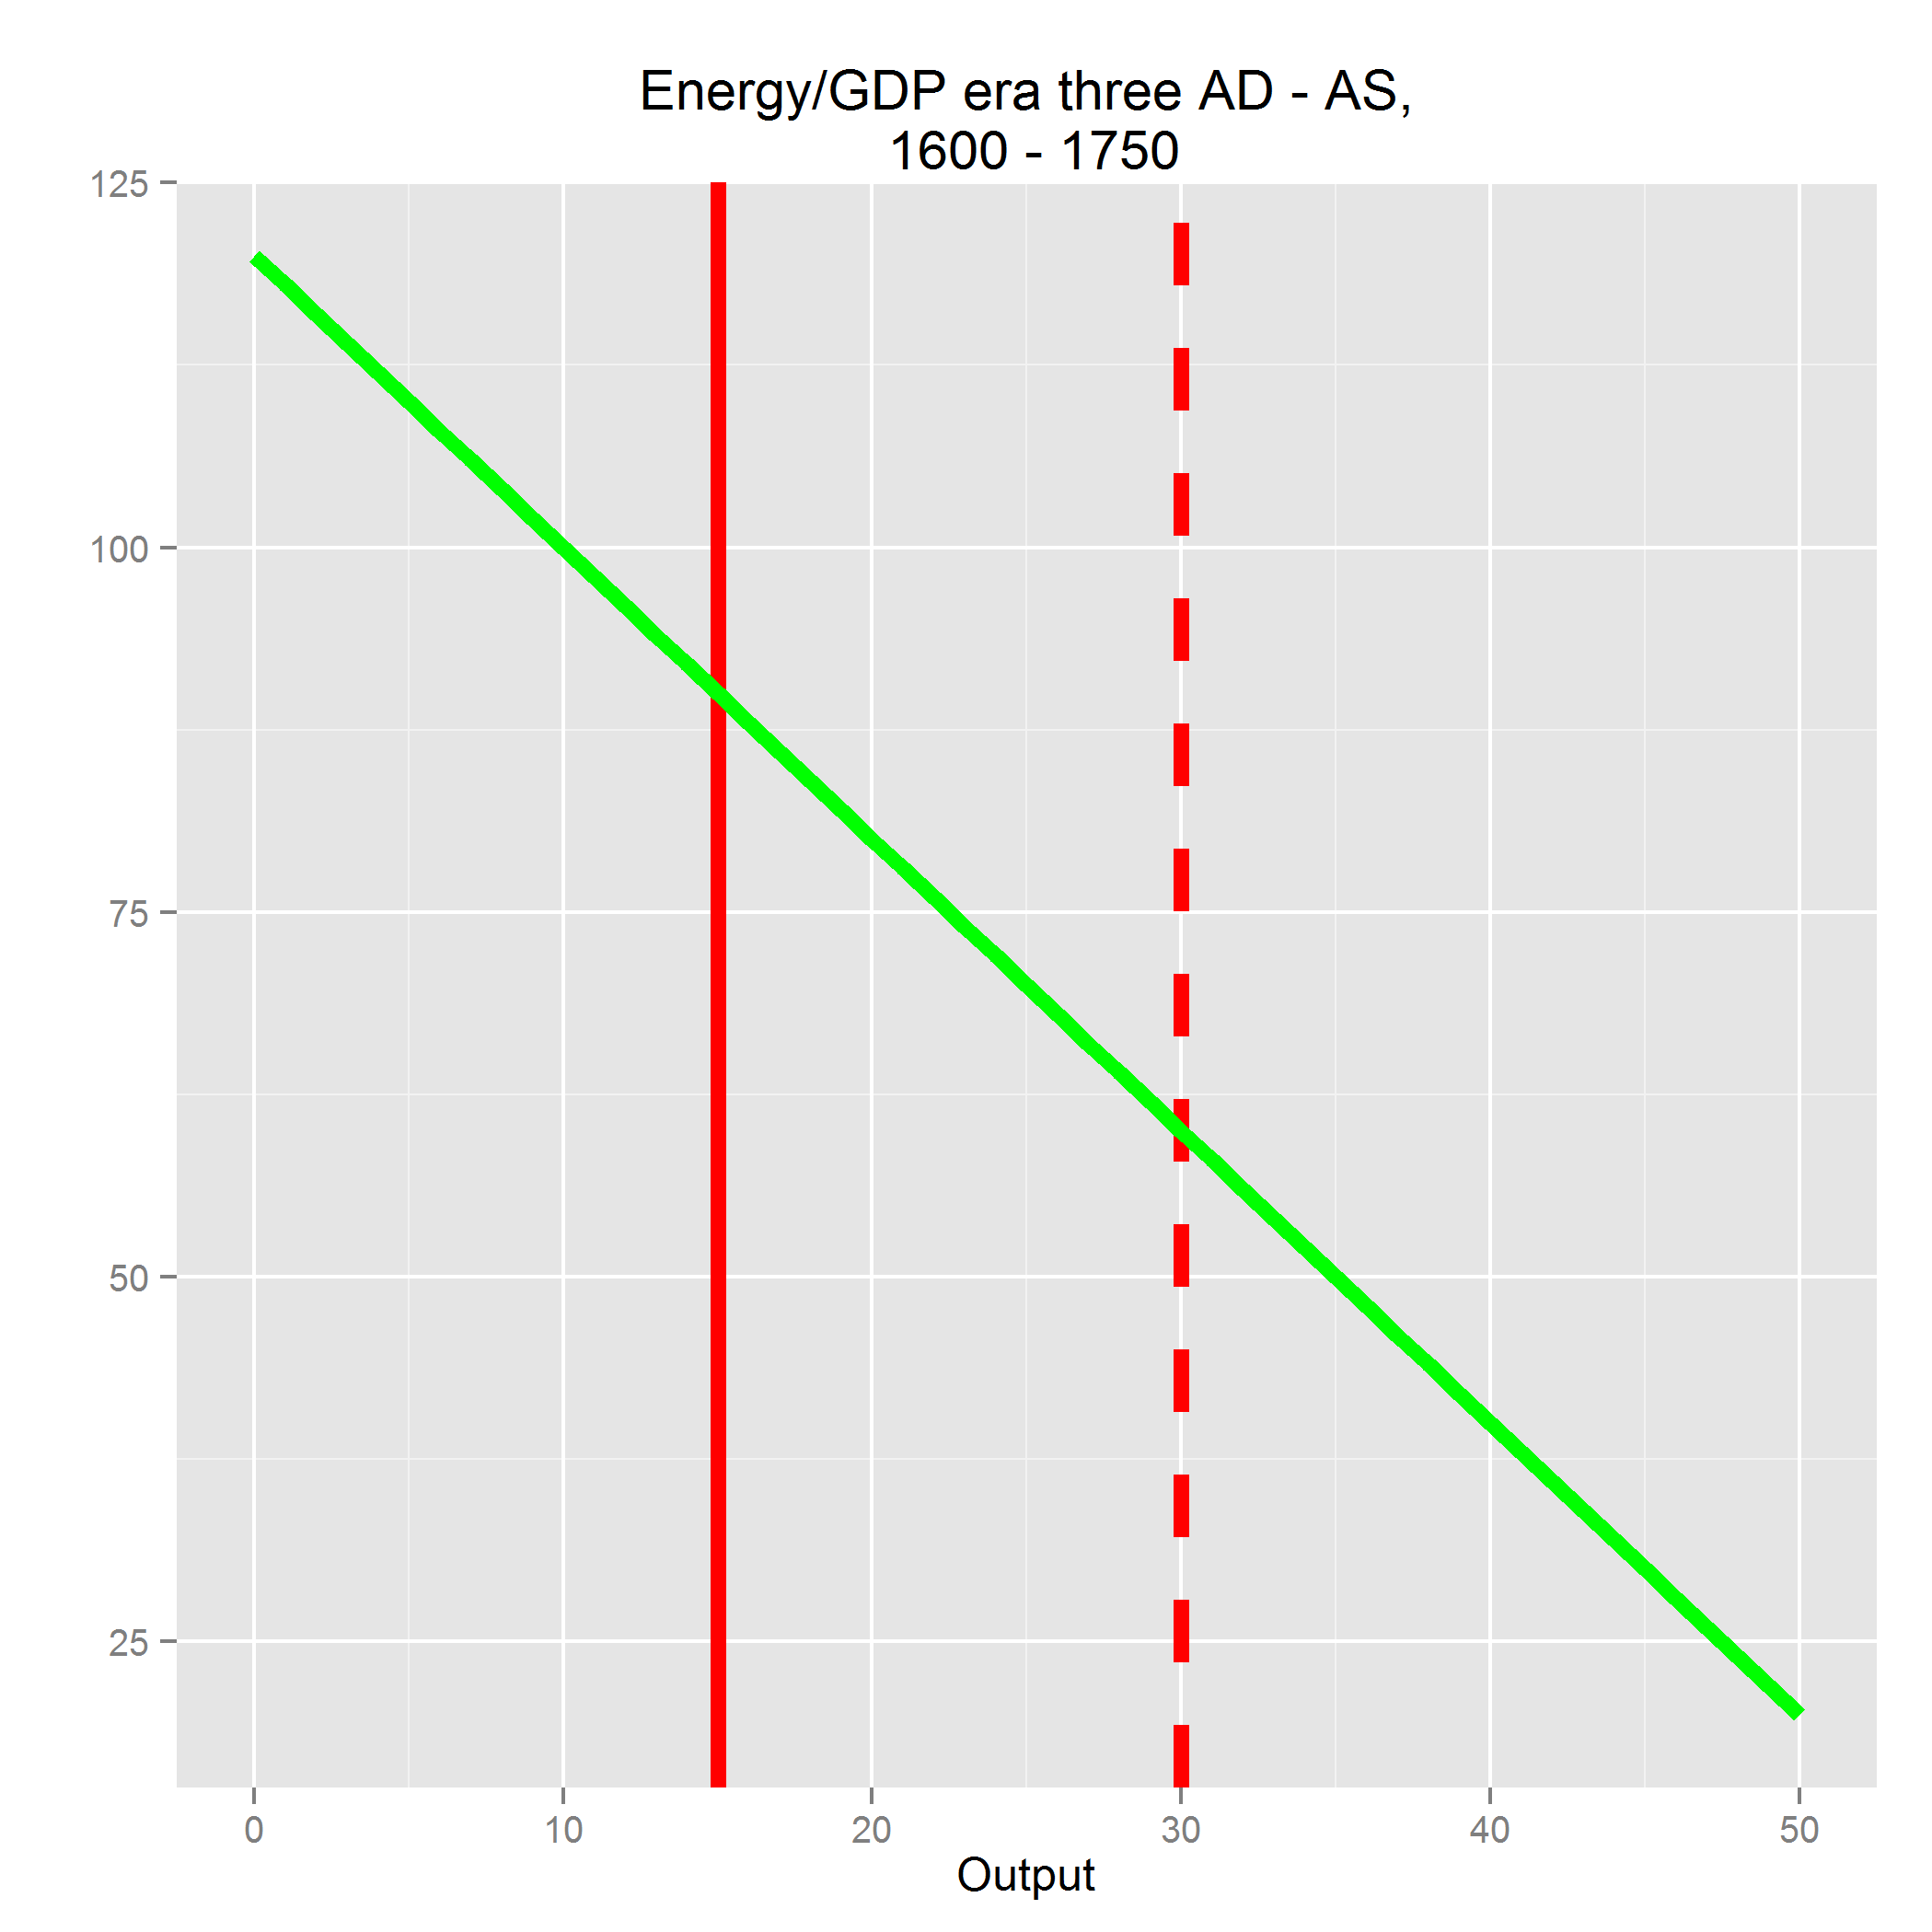
\includegraphics[height=0.35\textheight]{era3}}
		\mbox{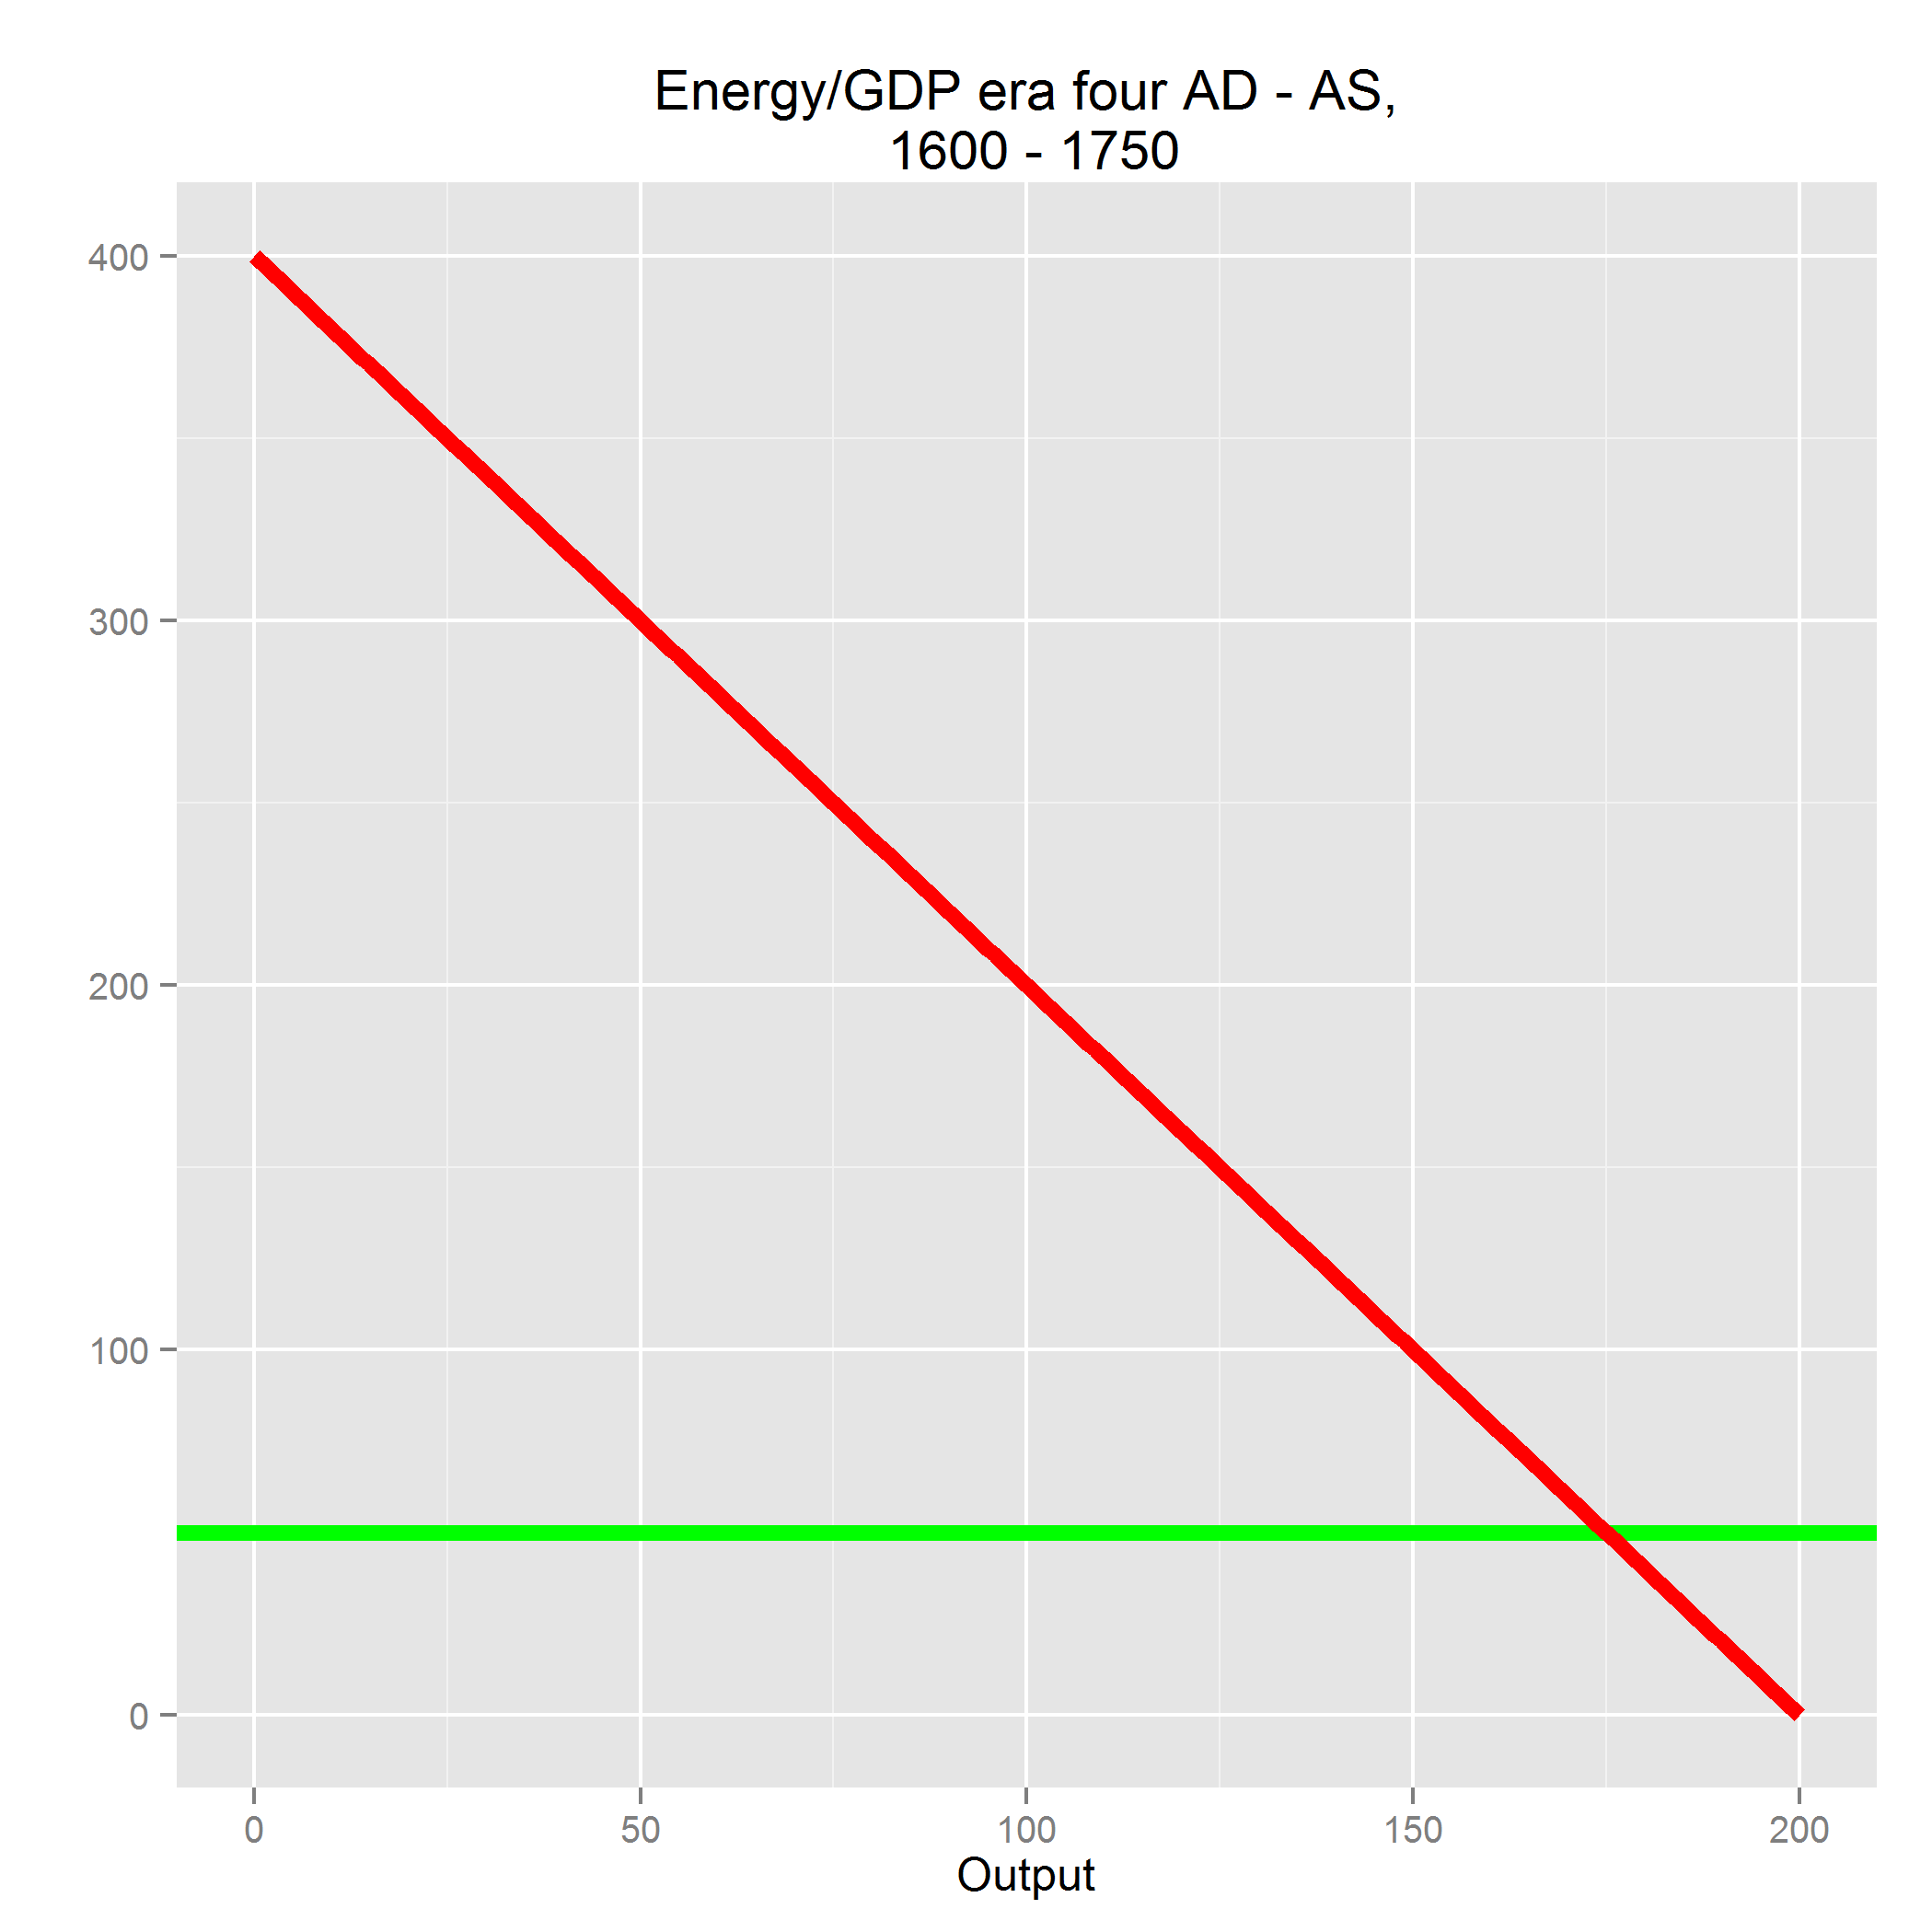
\includegraphics[height=0.35\textheight]{era4}}				
		}
		\end{figure}
\end{frame}

\begin{frame}
\frametitle{GDP/Energy regime one -- 1300-1500}
		\begin{figure}[p!]
%		\caption{Aggregate Supply - Aggregate Demand \\ Four energy/GDP regimes}
		\label{fig:asad}		
		\centerline{
		\mbox{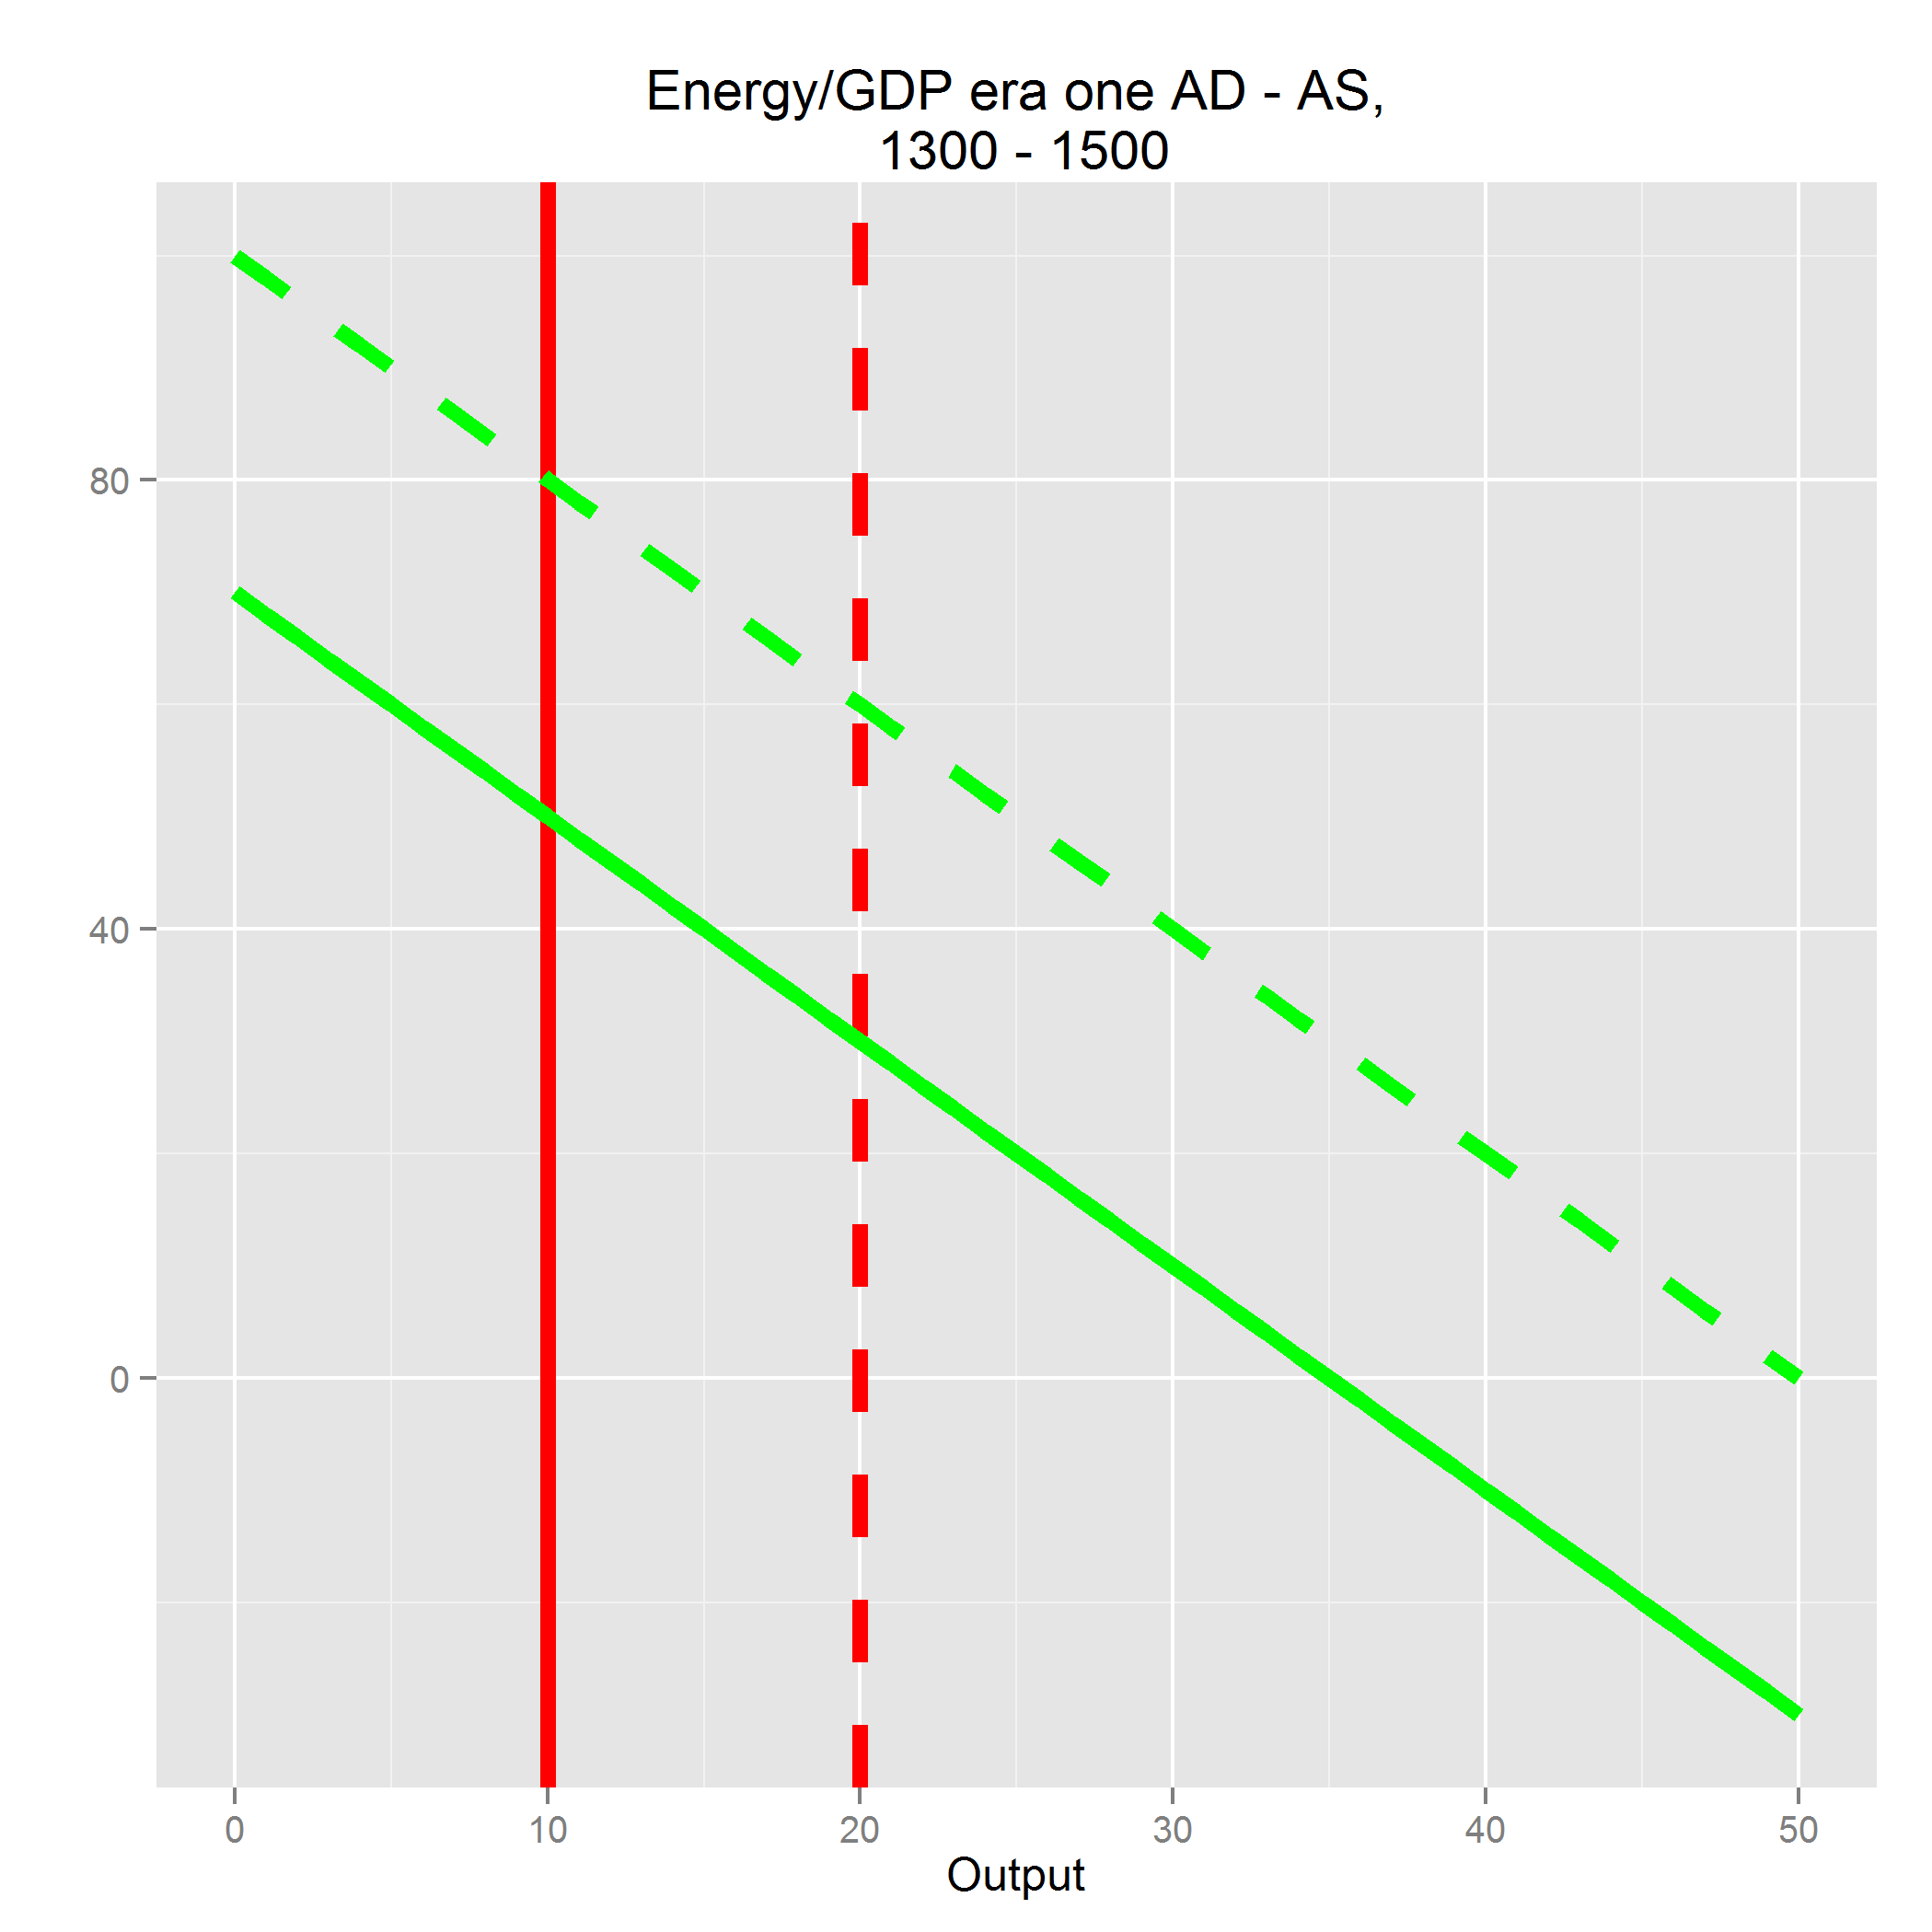
\includegraphics[height=0.5\textheight]{era1}}
		\mbox{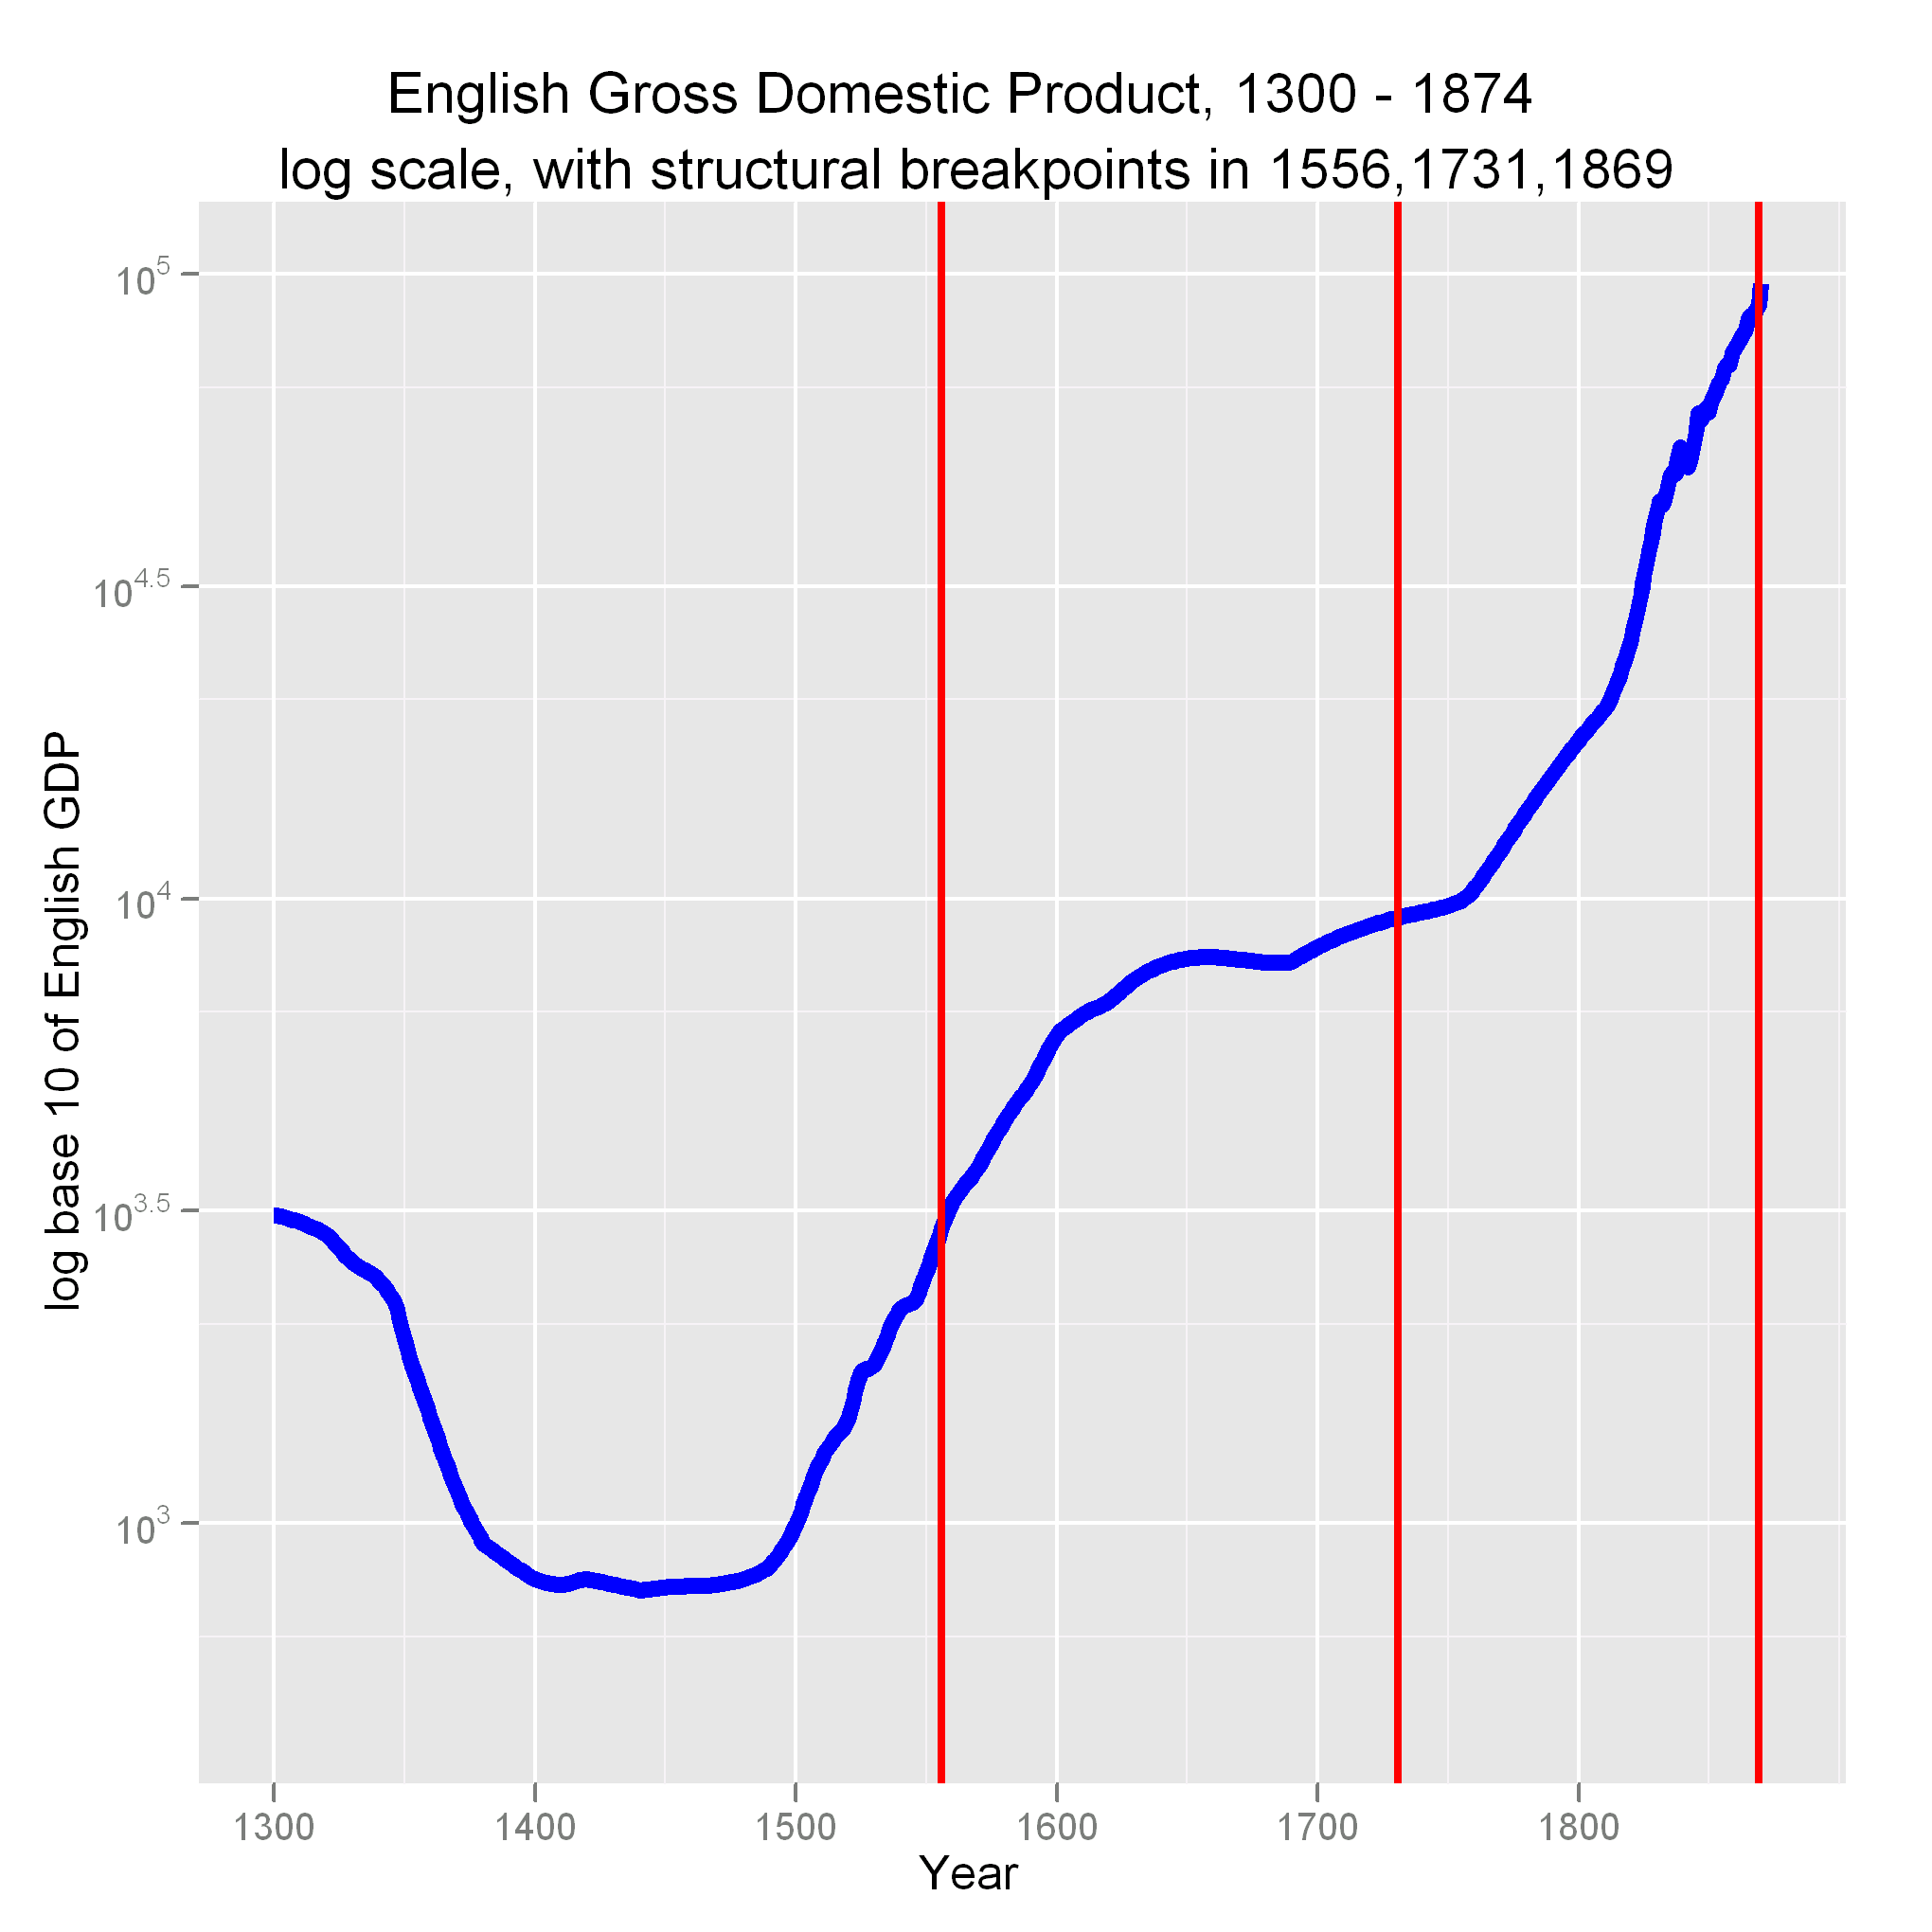
\includegraphics[height=0.5\textheight]{gbpgdplog}}
		\mbox{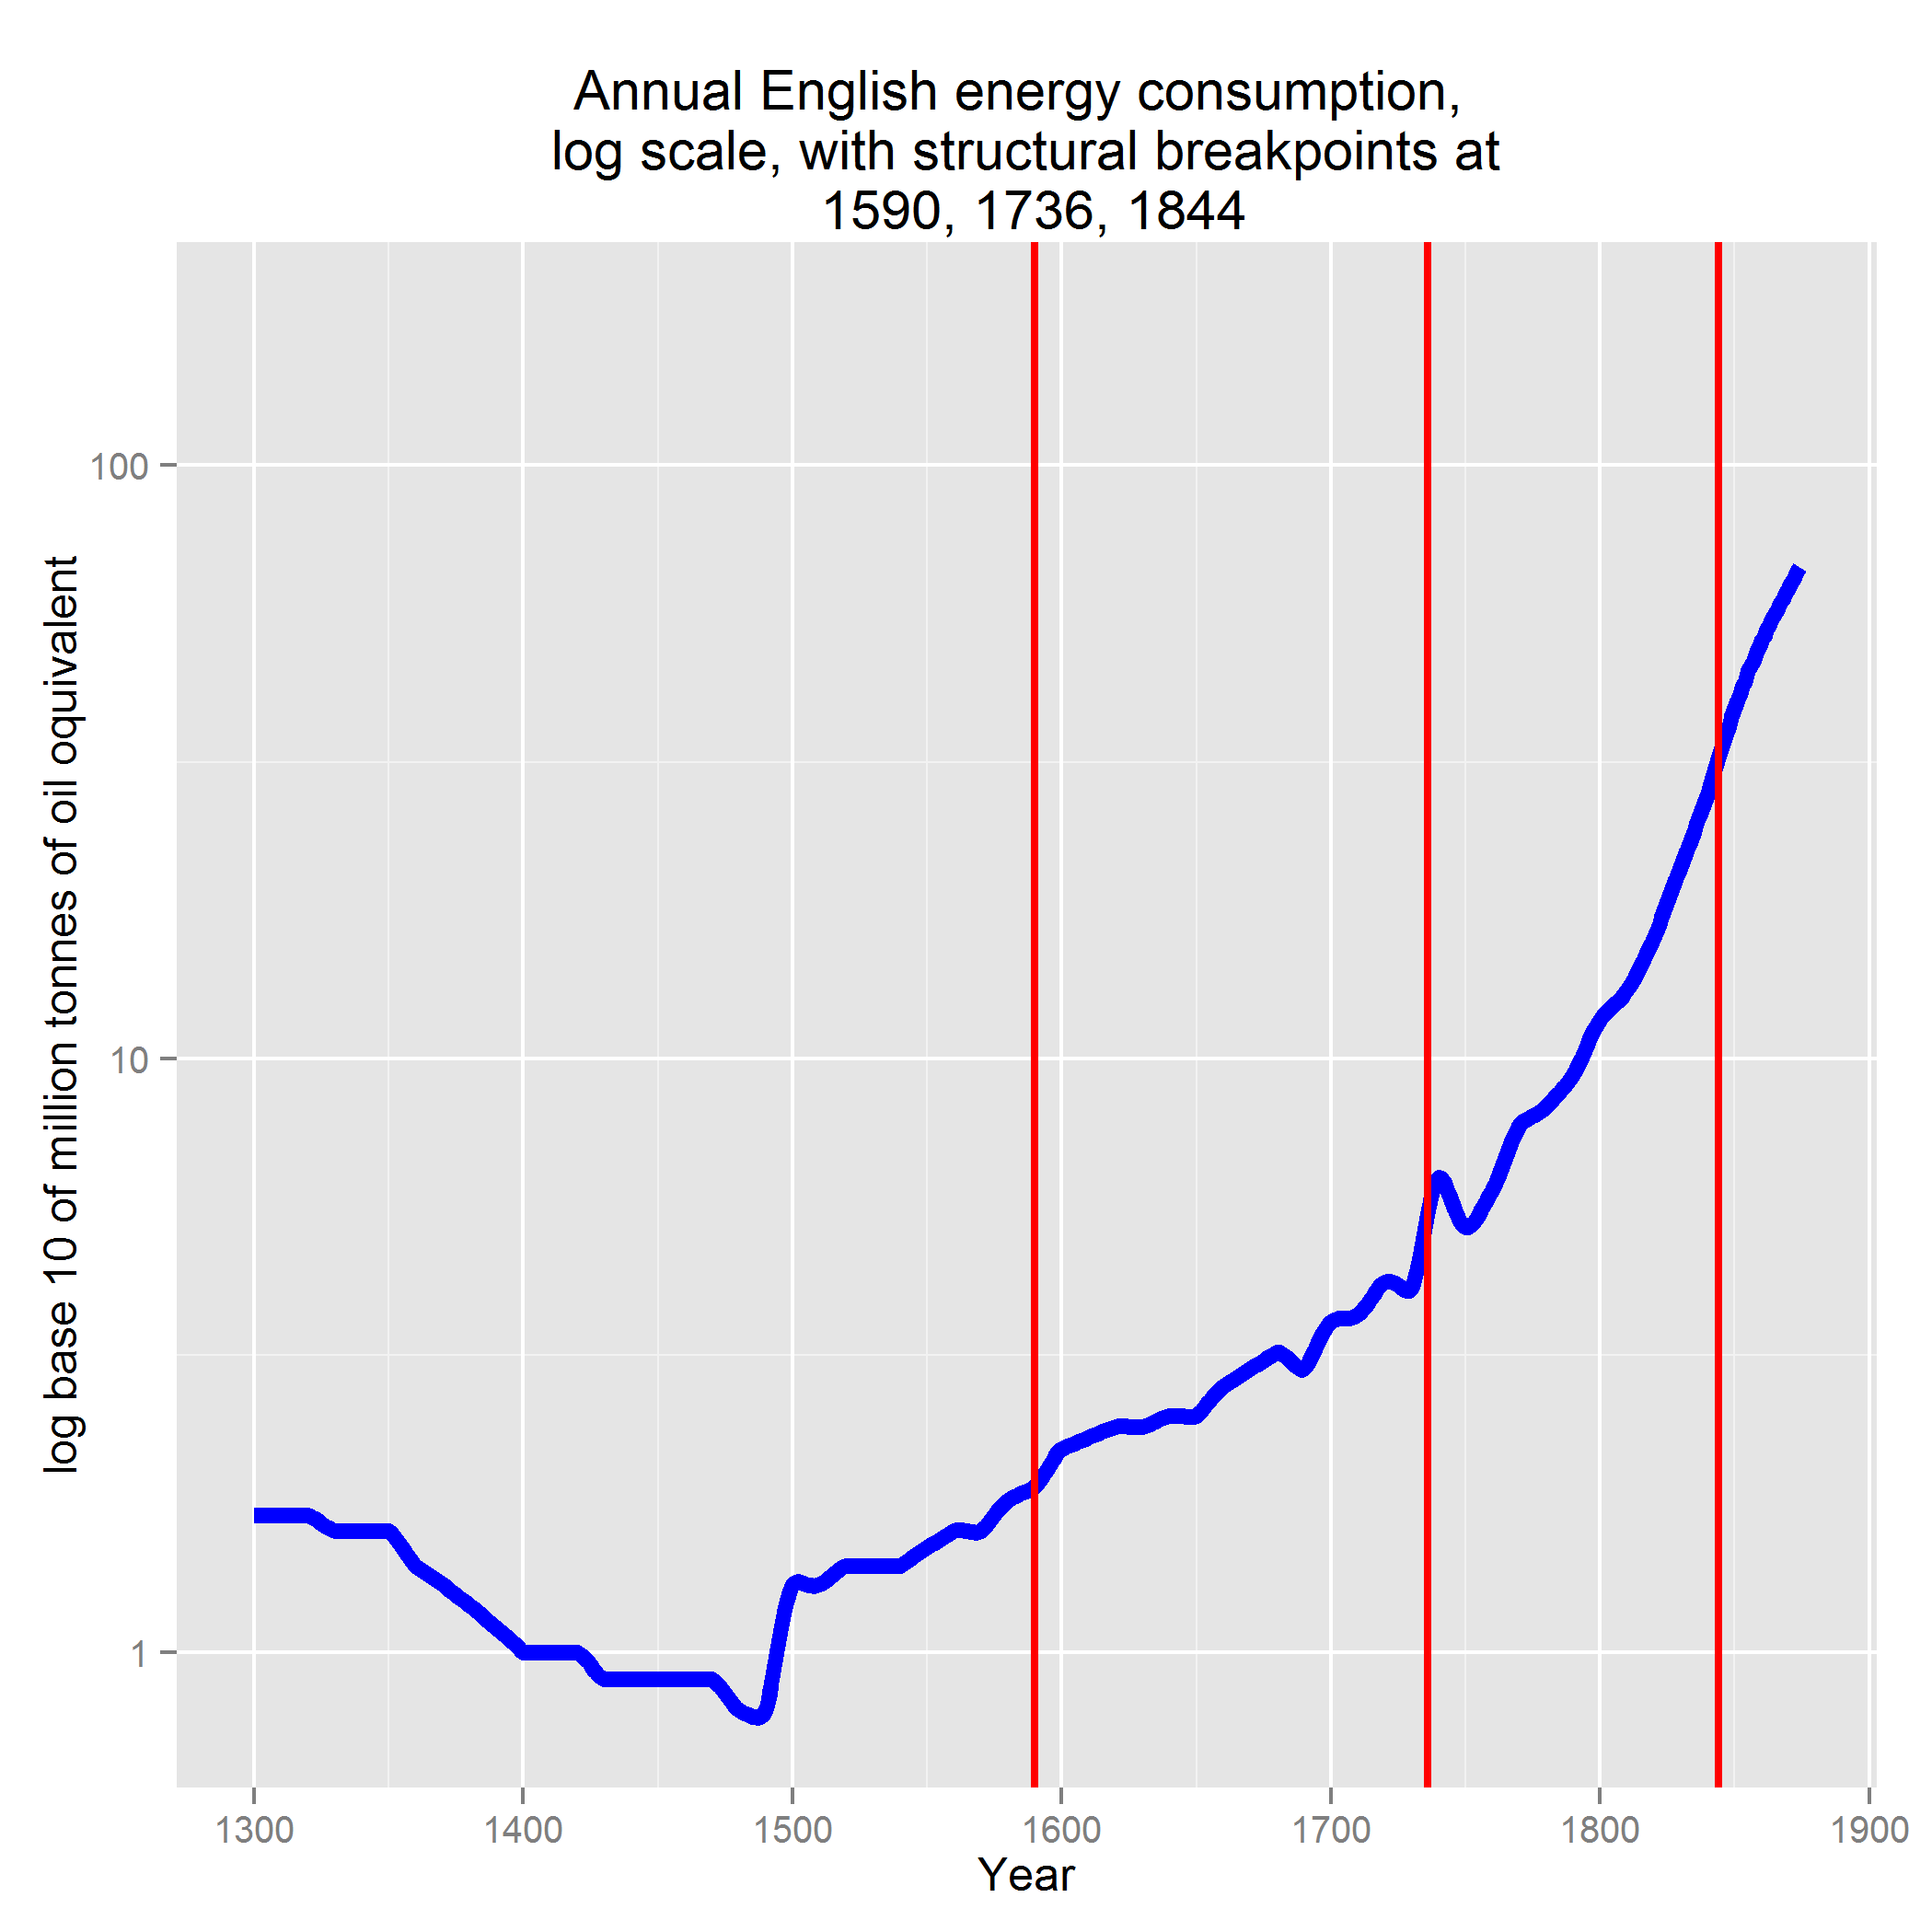
\includegraphics[height=0.5\textheight]{energyLog1}}
		}
		\end{figure} \vspace*{-0.4in}
Black Death recovery -- higher wage support, population recovery\\
Medieval Warming Epoch -- agricultural expansion, higher population\\
European Marriage Pattern -- reduced nuptiality, higher real wage\\
Demand and supply expansion\\
\end{frame}

\begin{frame}
\frametitle{GDP/Energy regime two -- 1500-1600}
		\begin{figure}[p!]
%		\caption{Aggregate Supply - Aggregate Demand \\ Four energy/GDP regimes}
		\label{fig:asad}		
		\centerline{
		\mbox{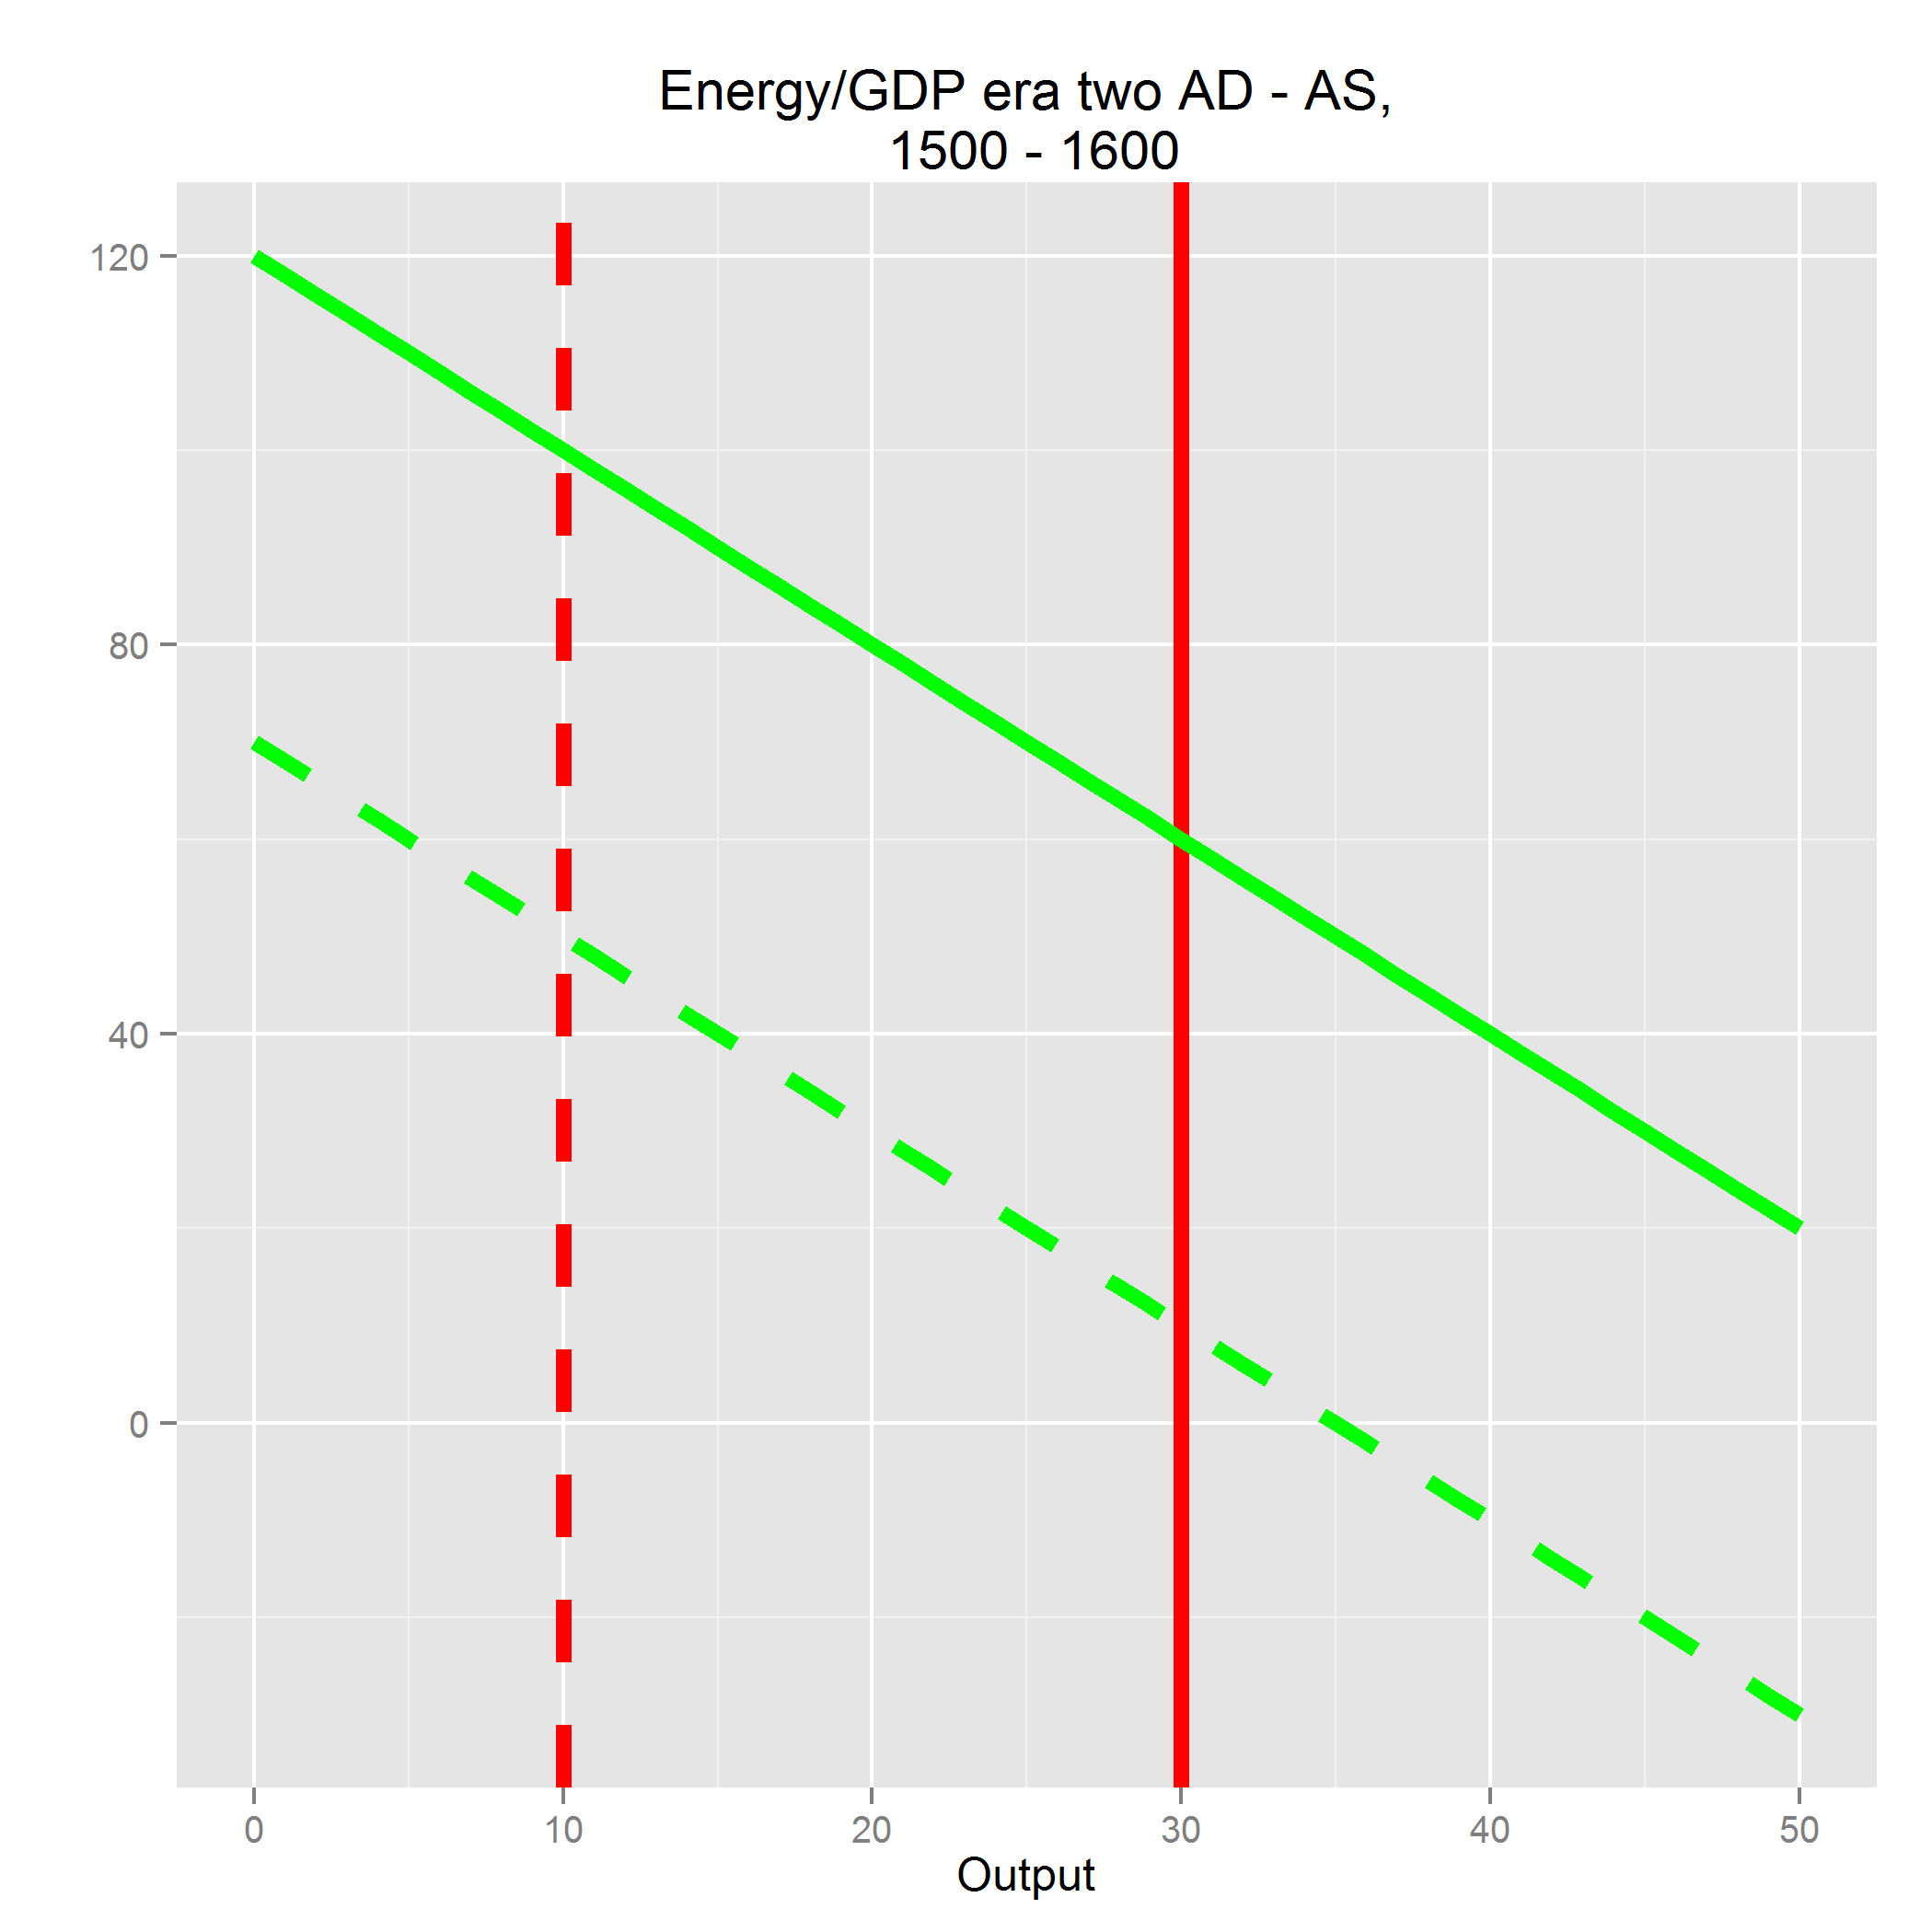
\includegraphics[height=0.5\textheight]{era2}}
		\mbox{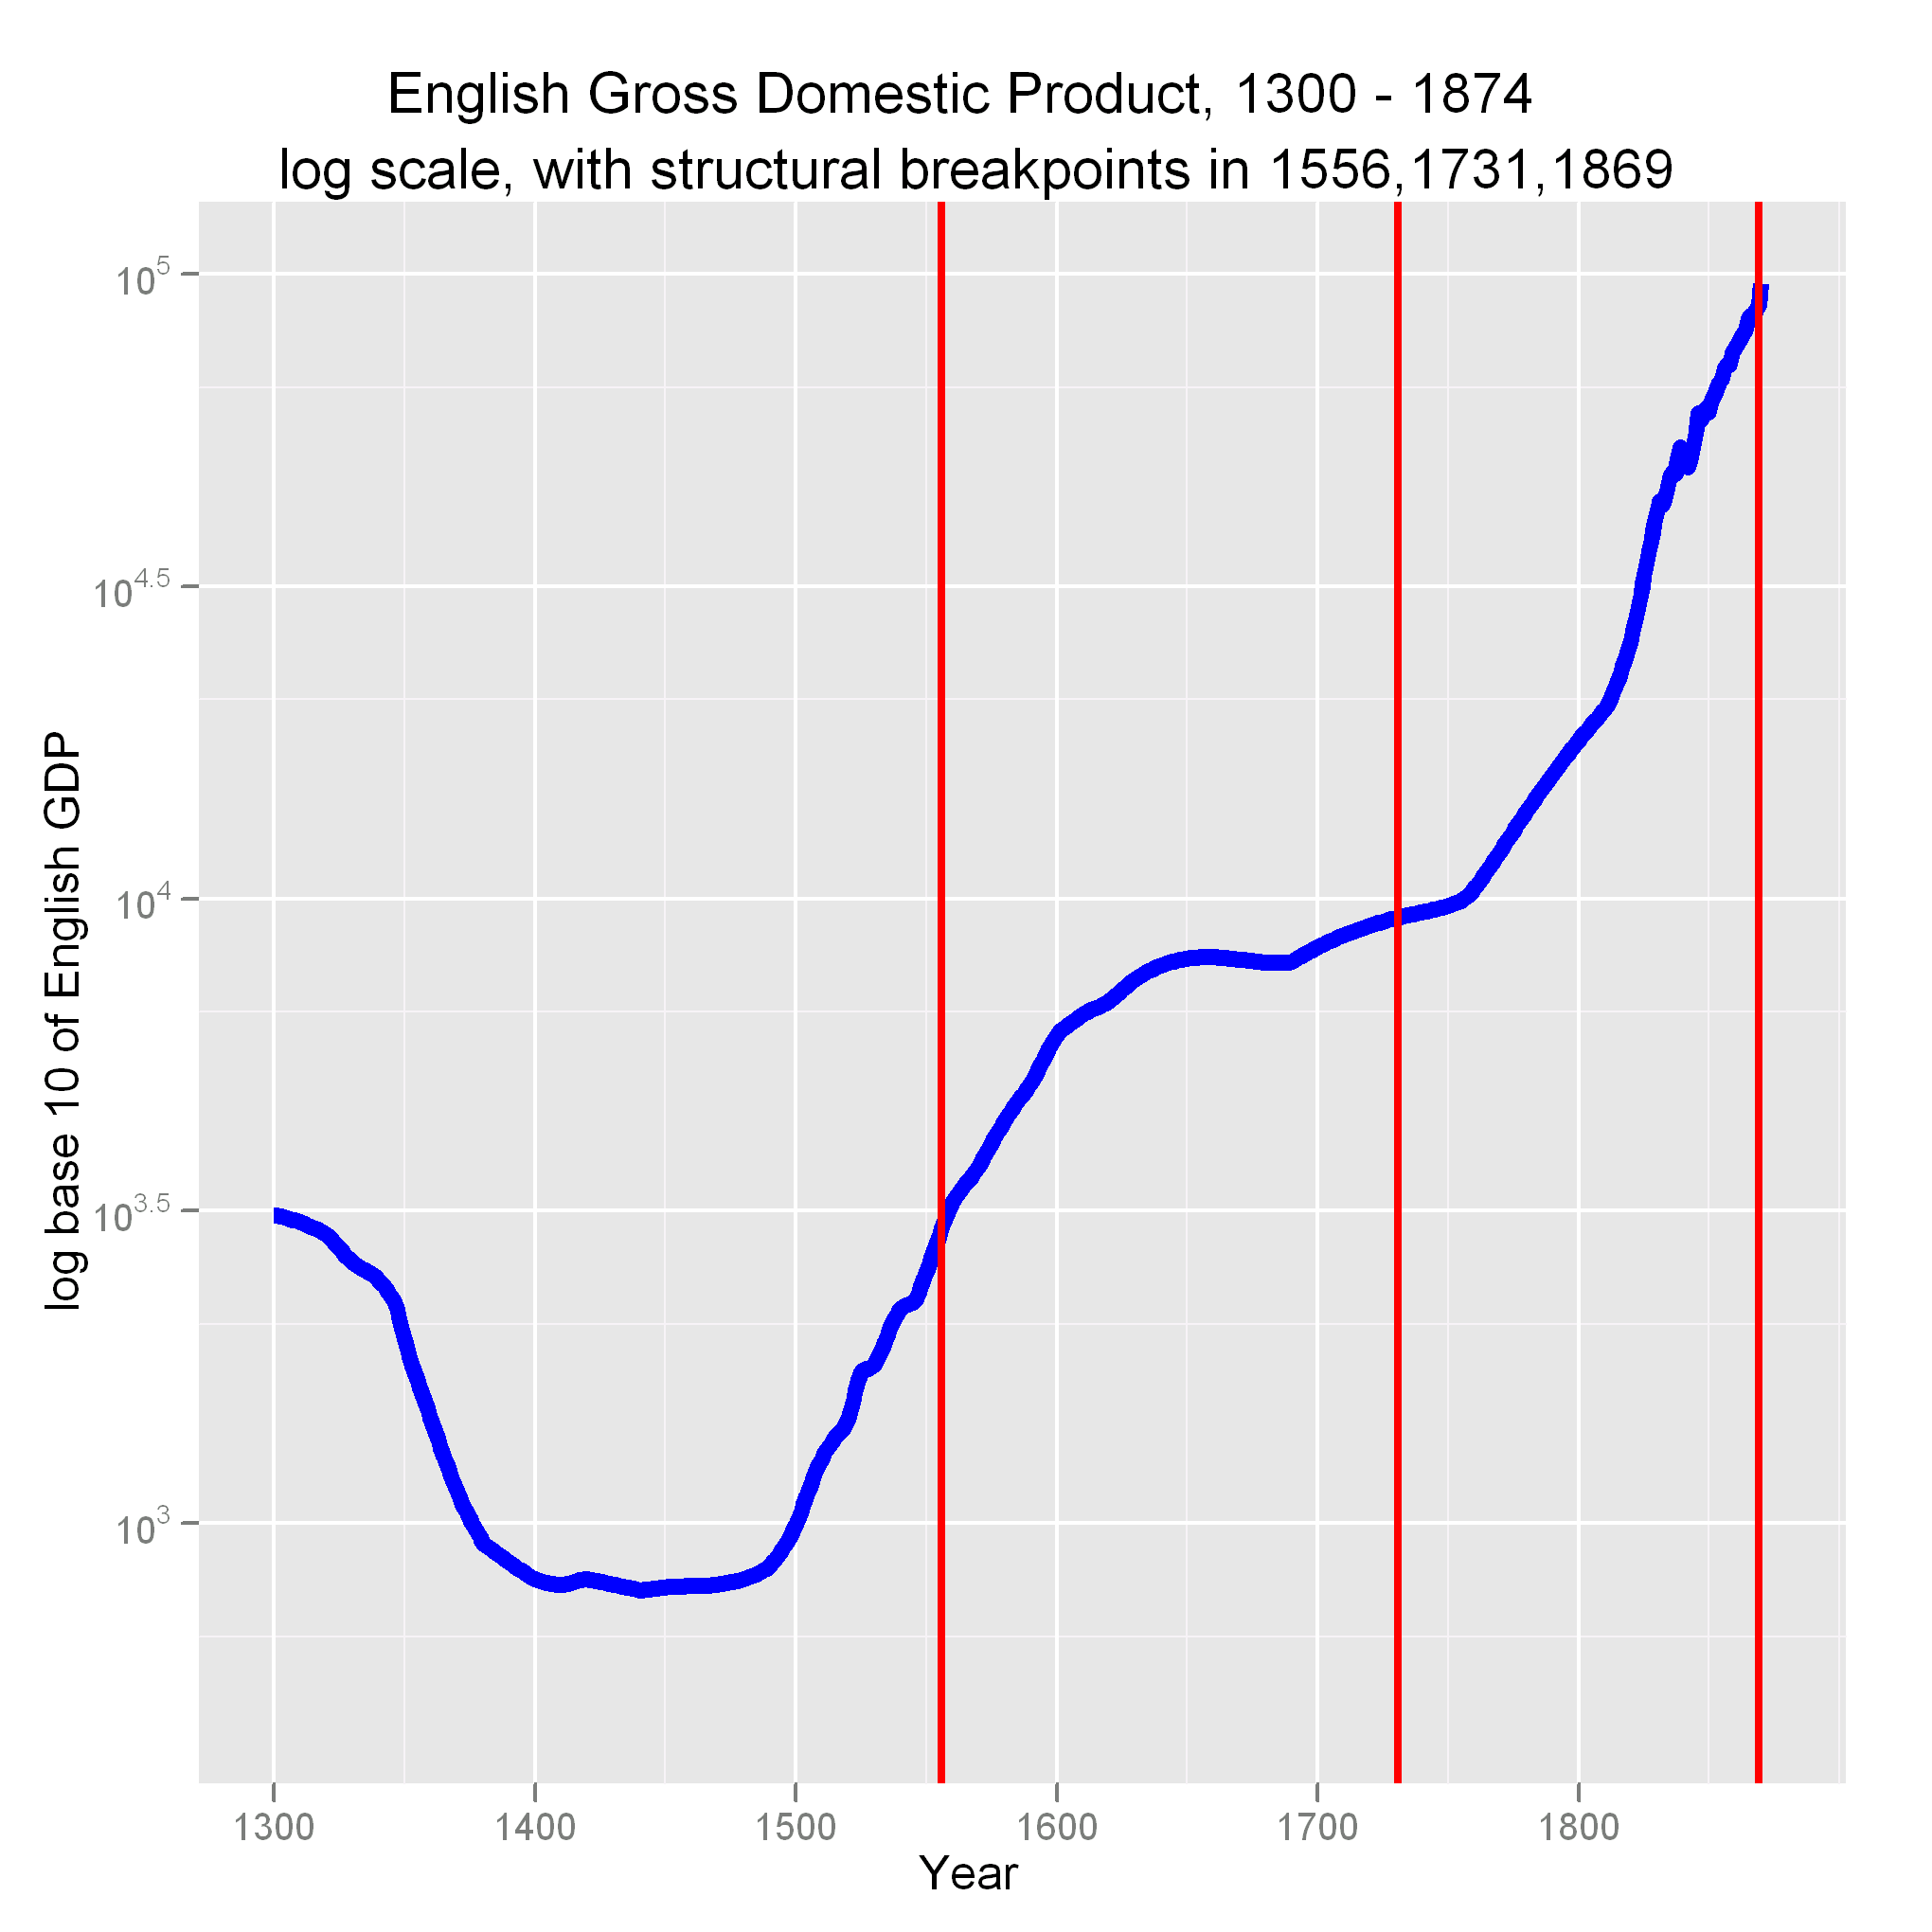
\includegraphics[height=0.5\textheight]{gbpgdplog}}
		\mbox{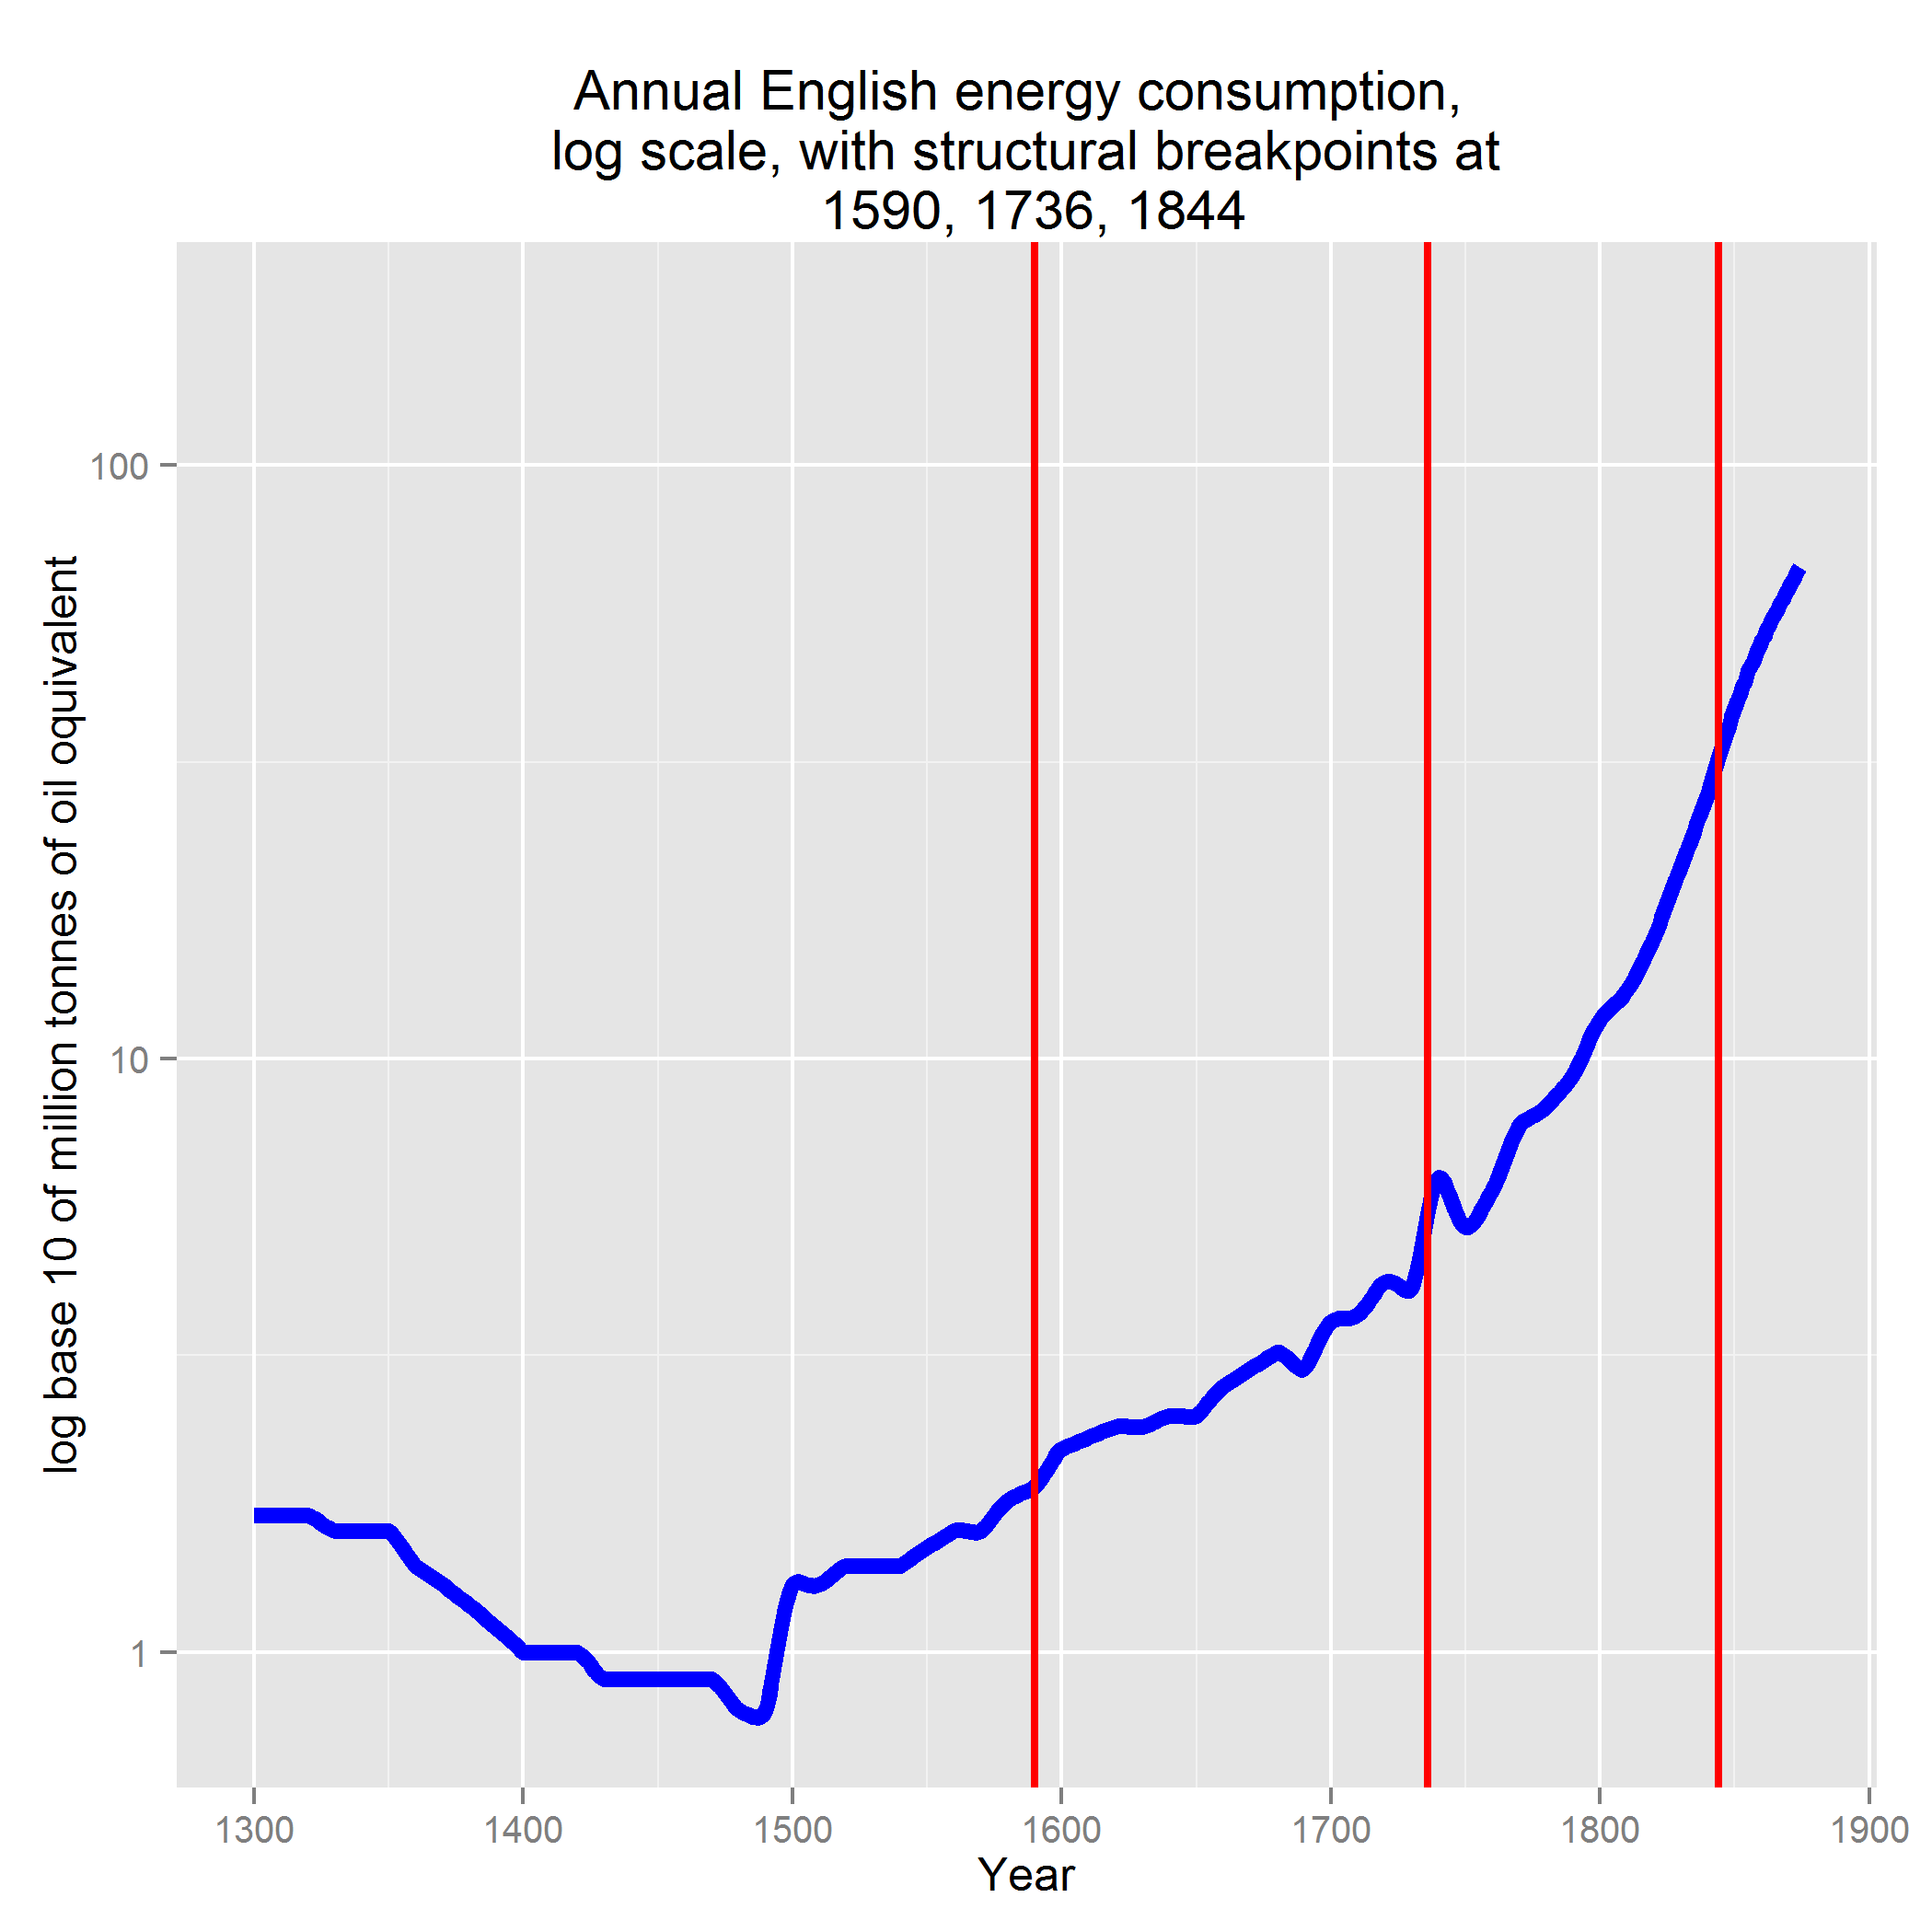
\includegraphics[height=0.5\textheight]{energyLog1}}
		}
		\end{figure} \vspace*{-0.4in}
Benign climate -- agriculture, real wage, population rise\\
Beginning of first energy crisis -- deforestation\\
Demand and supply expansion\\
\end{frame}

\begin{frame}
\frametitle{GDP/Energy regime three -- 1600-1750}
		\begin{figure}[p!]
%		\caption{Aggregate Supply - Aggregate Demand \\ Four energy/GDP regimes}
		\label{fig:asad}		
		\centerline{
		\mbox{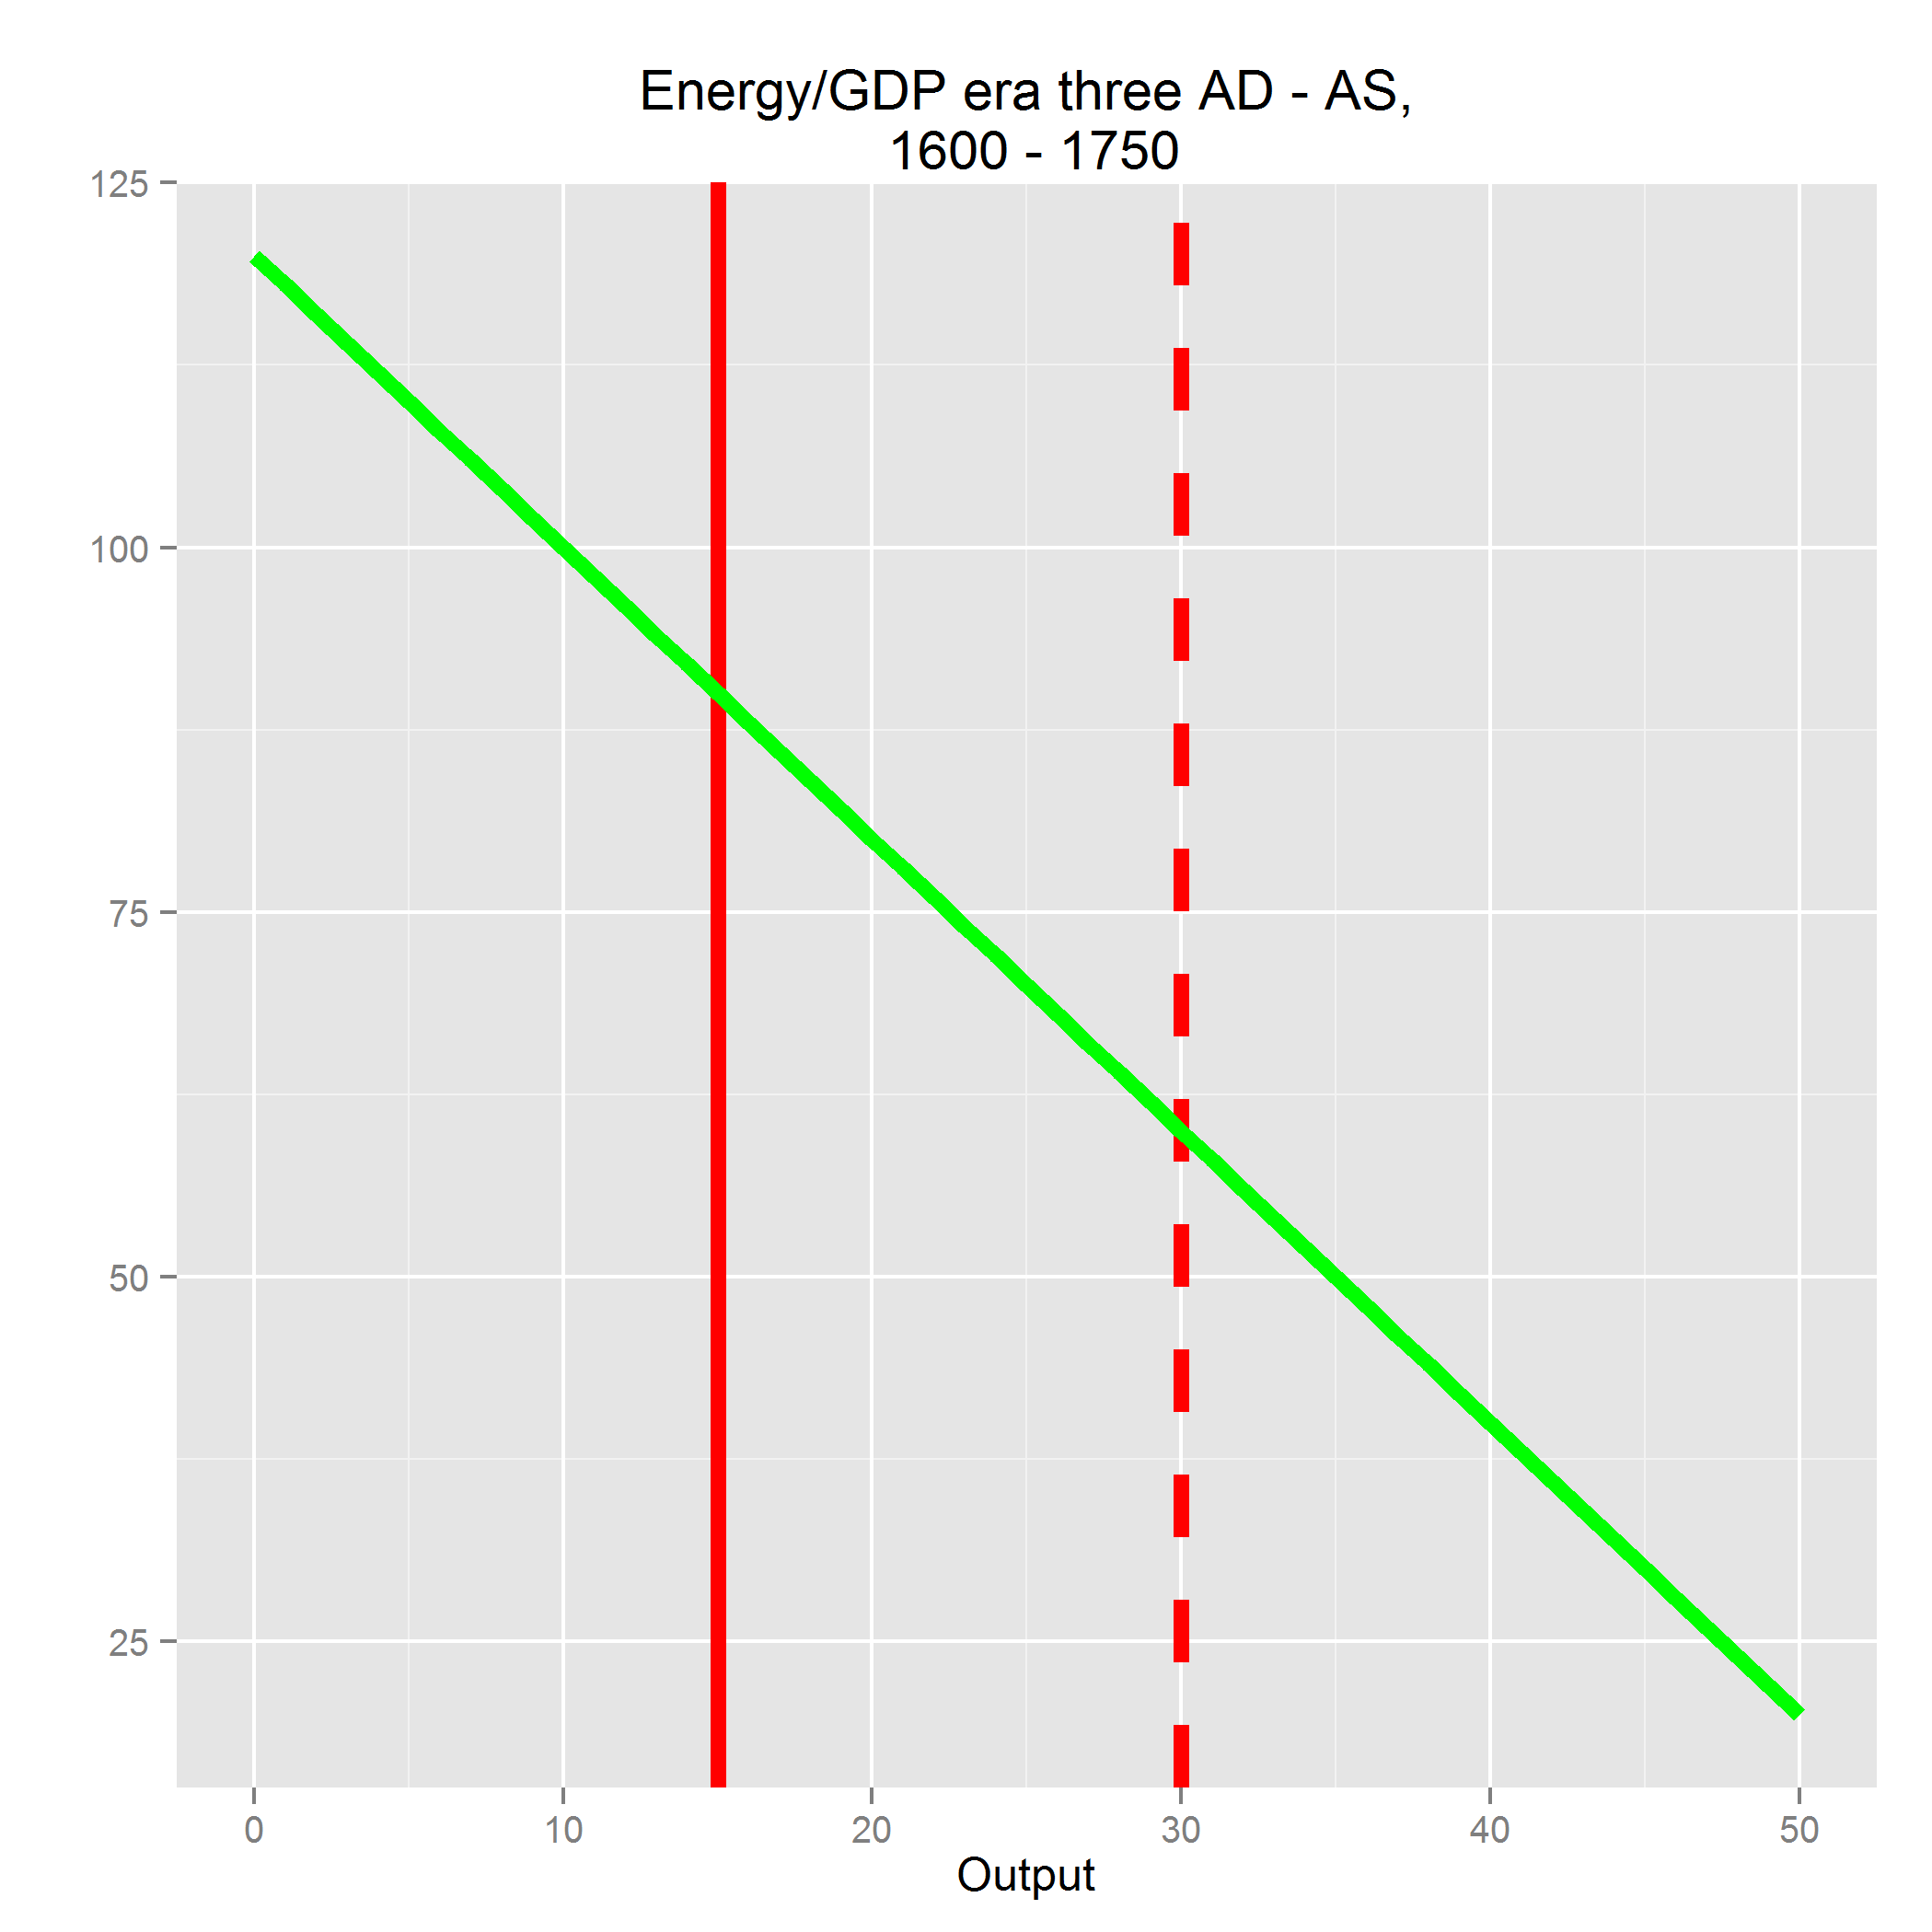
\includegraphics[height=0.5\textheight]{era3}}
		\mbox{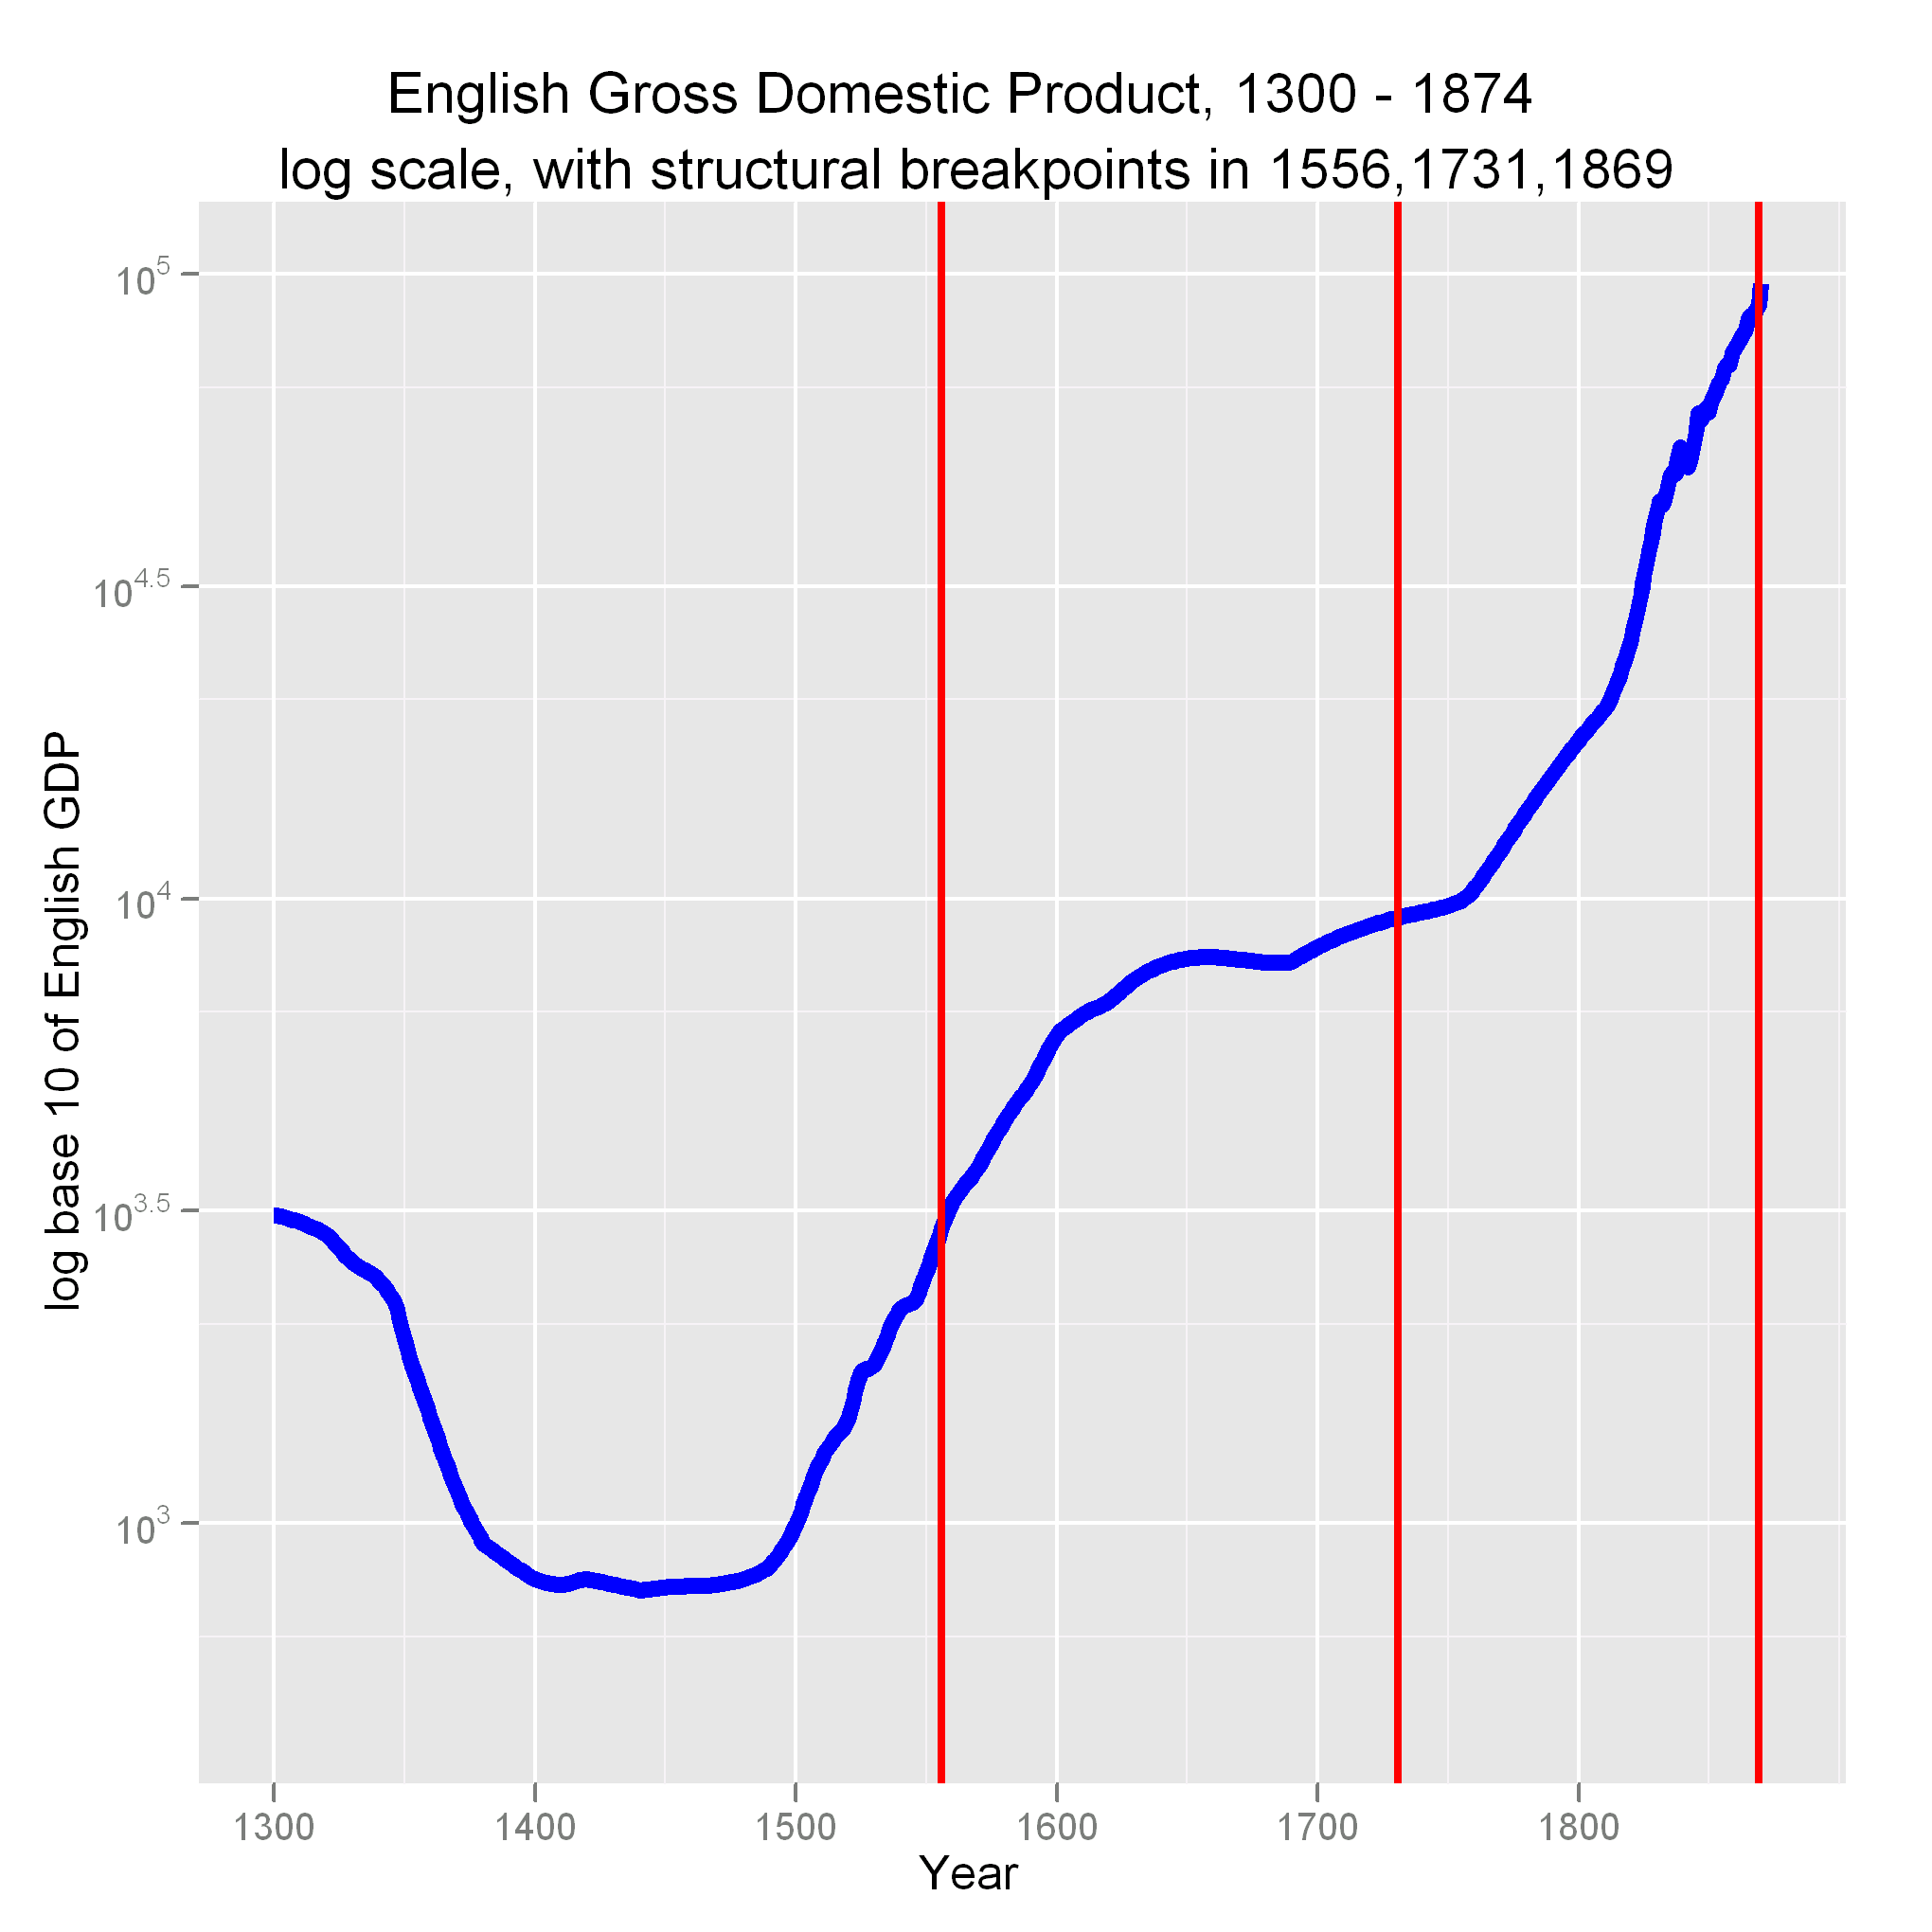
\includegraphics[height=0.5\textheight]{gbpgdplog}}
		\mbox{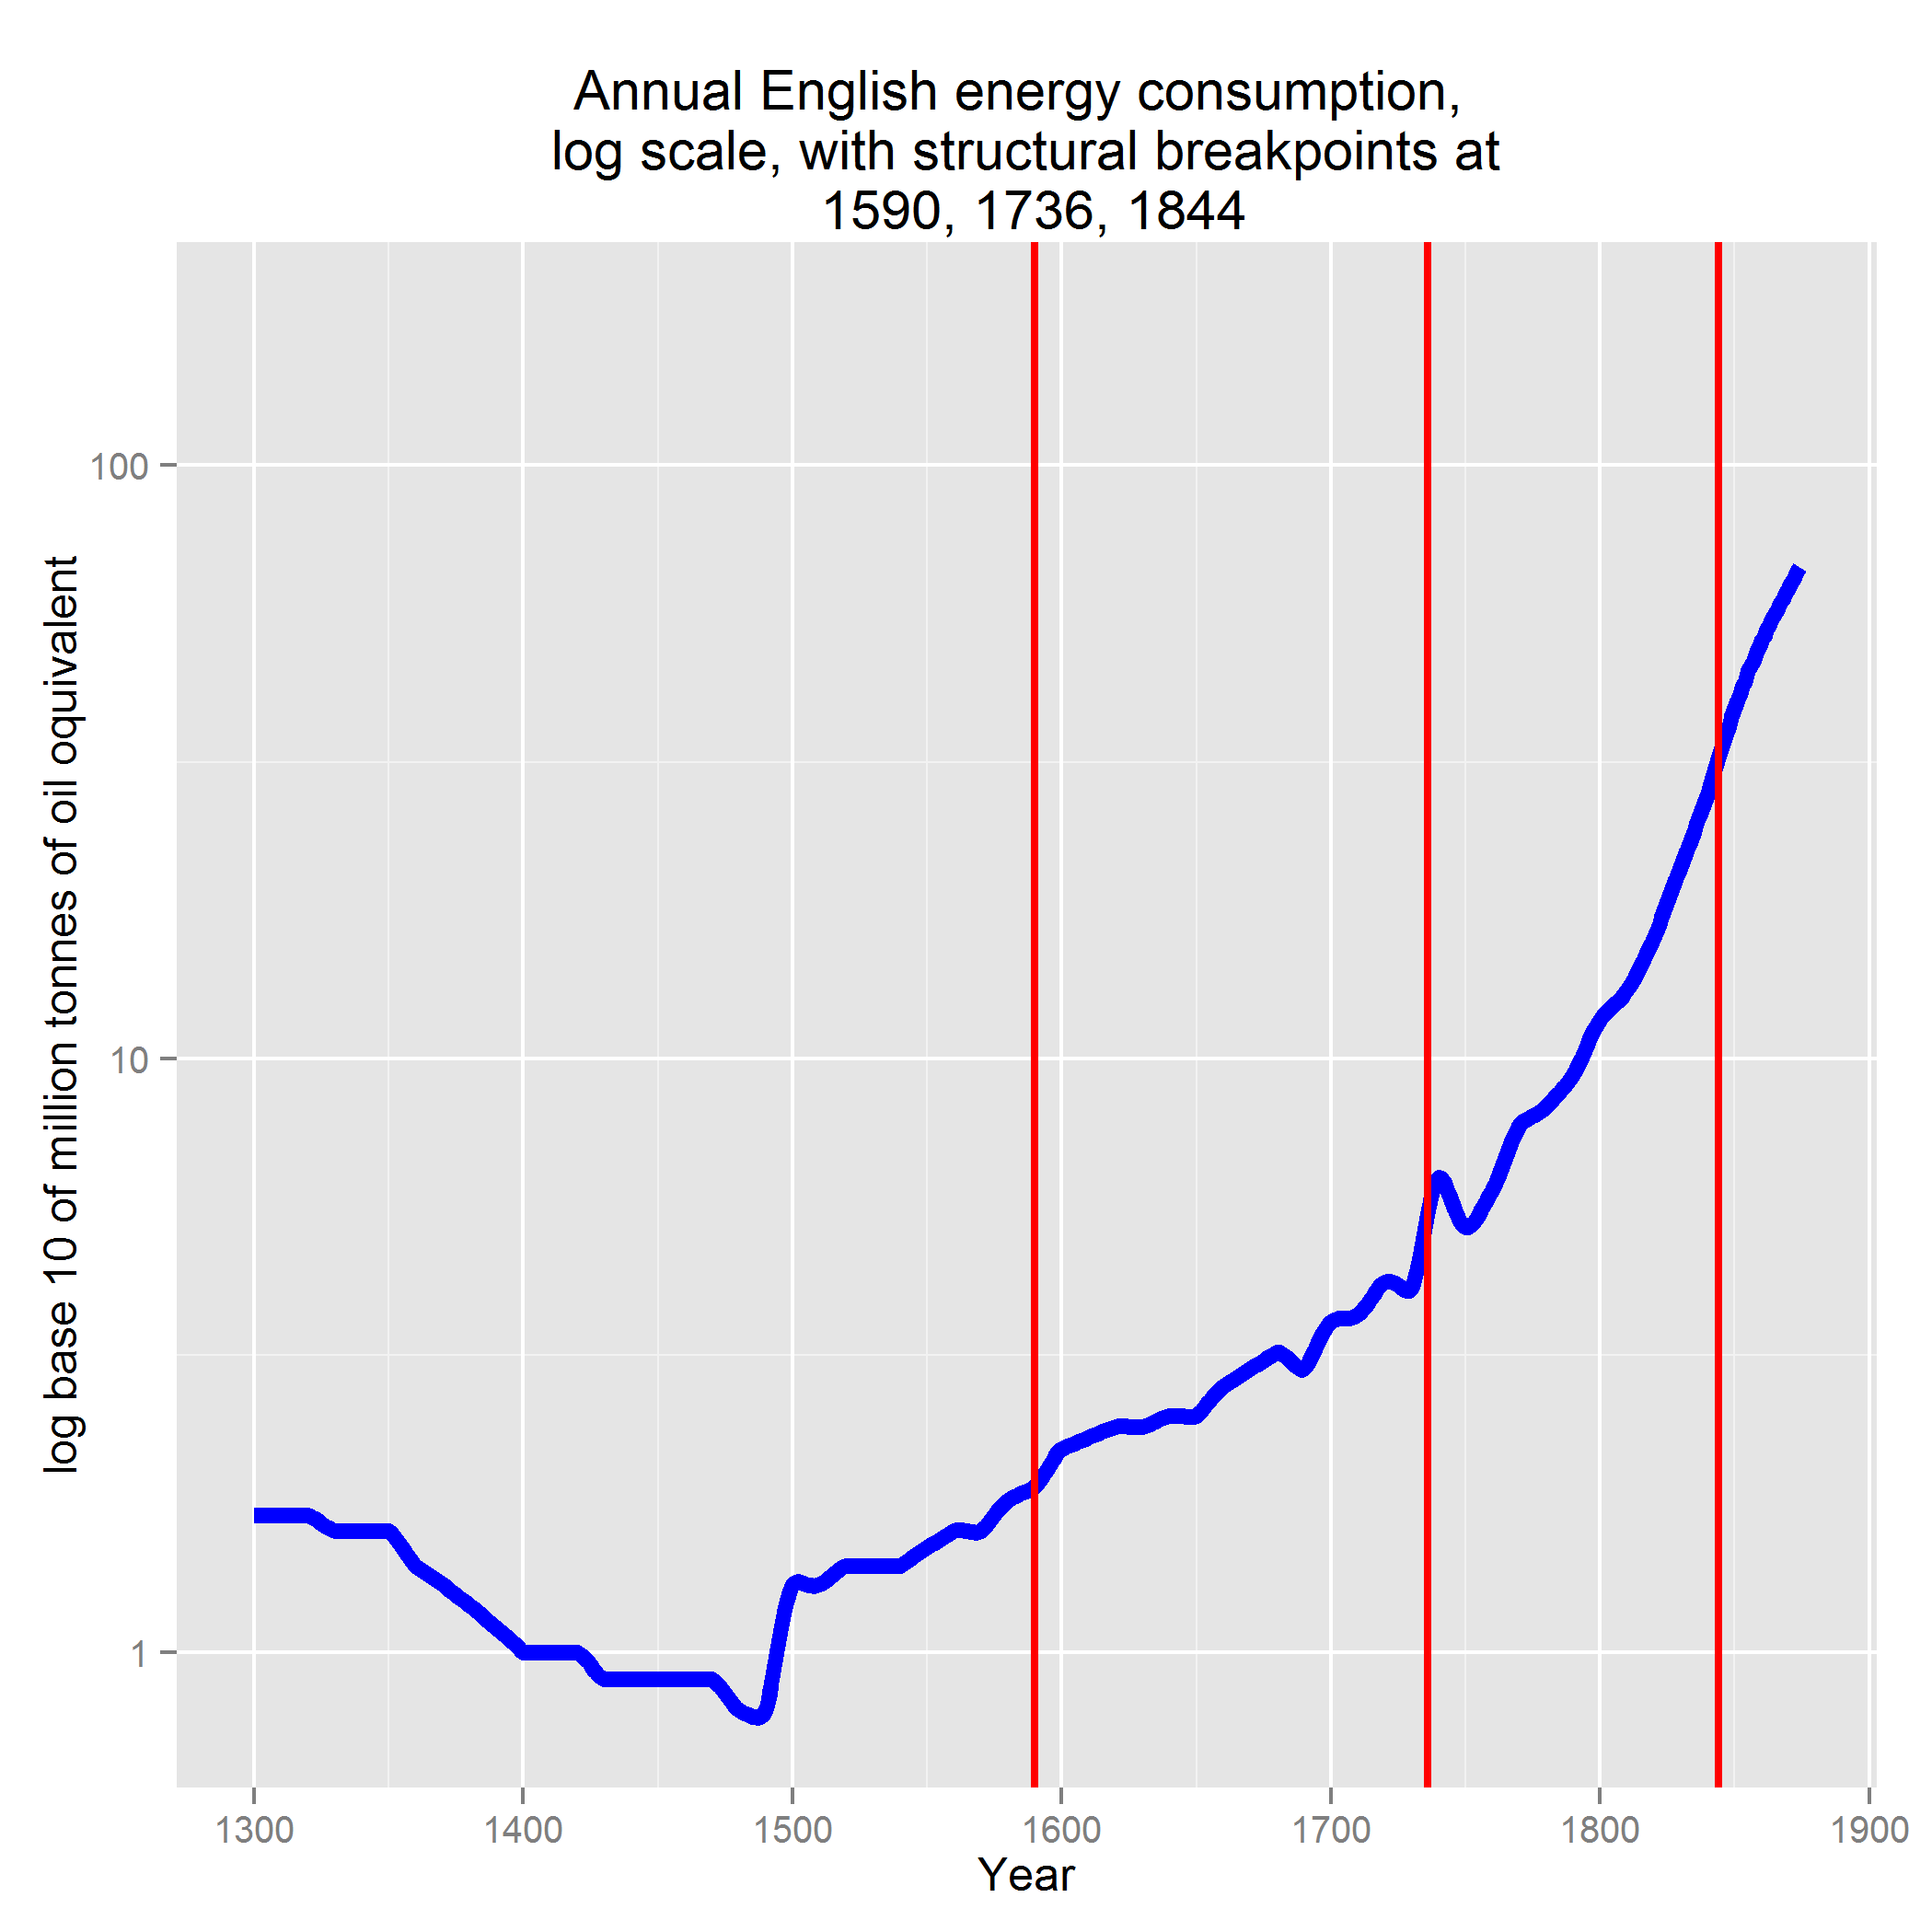
\includegraphics[height=0.5\textheight]{energyLog1}}
		}
		\end{figure} \vspace*{-0.4in}
Little Ice Age -- agricultural shrinkage\\
Famine, Pestilence, Wars\\
"Global Crisis" (Parker) -- 30 percent global population decline\\
"General crisis" (Hugh Trevor-Roper)\\
Demand and supply shrinkage\\
First energy revolution -- substitute coal for wood\\
\end{frame}

\begin{frame}
\frametitle{GDP/Energy regime four -- 1750-1873}
		\begin{figure}[p!]
%		\caption{Aggregate Supply - Aggregate Demand \\ Four energy/GDP regimes}
		\label{fig:asad}		
		\centerline{
		\mbox{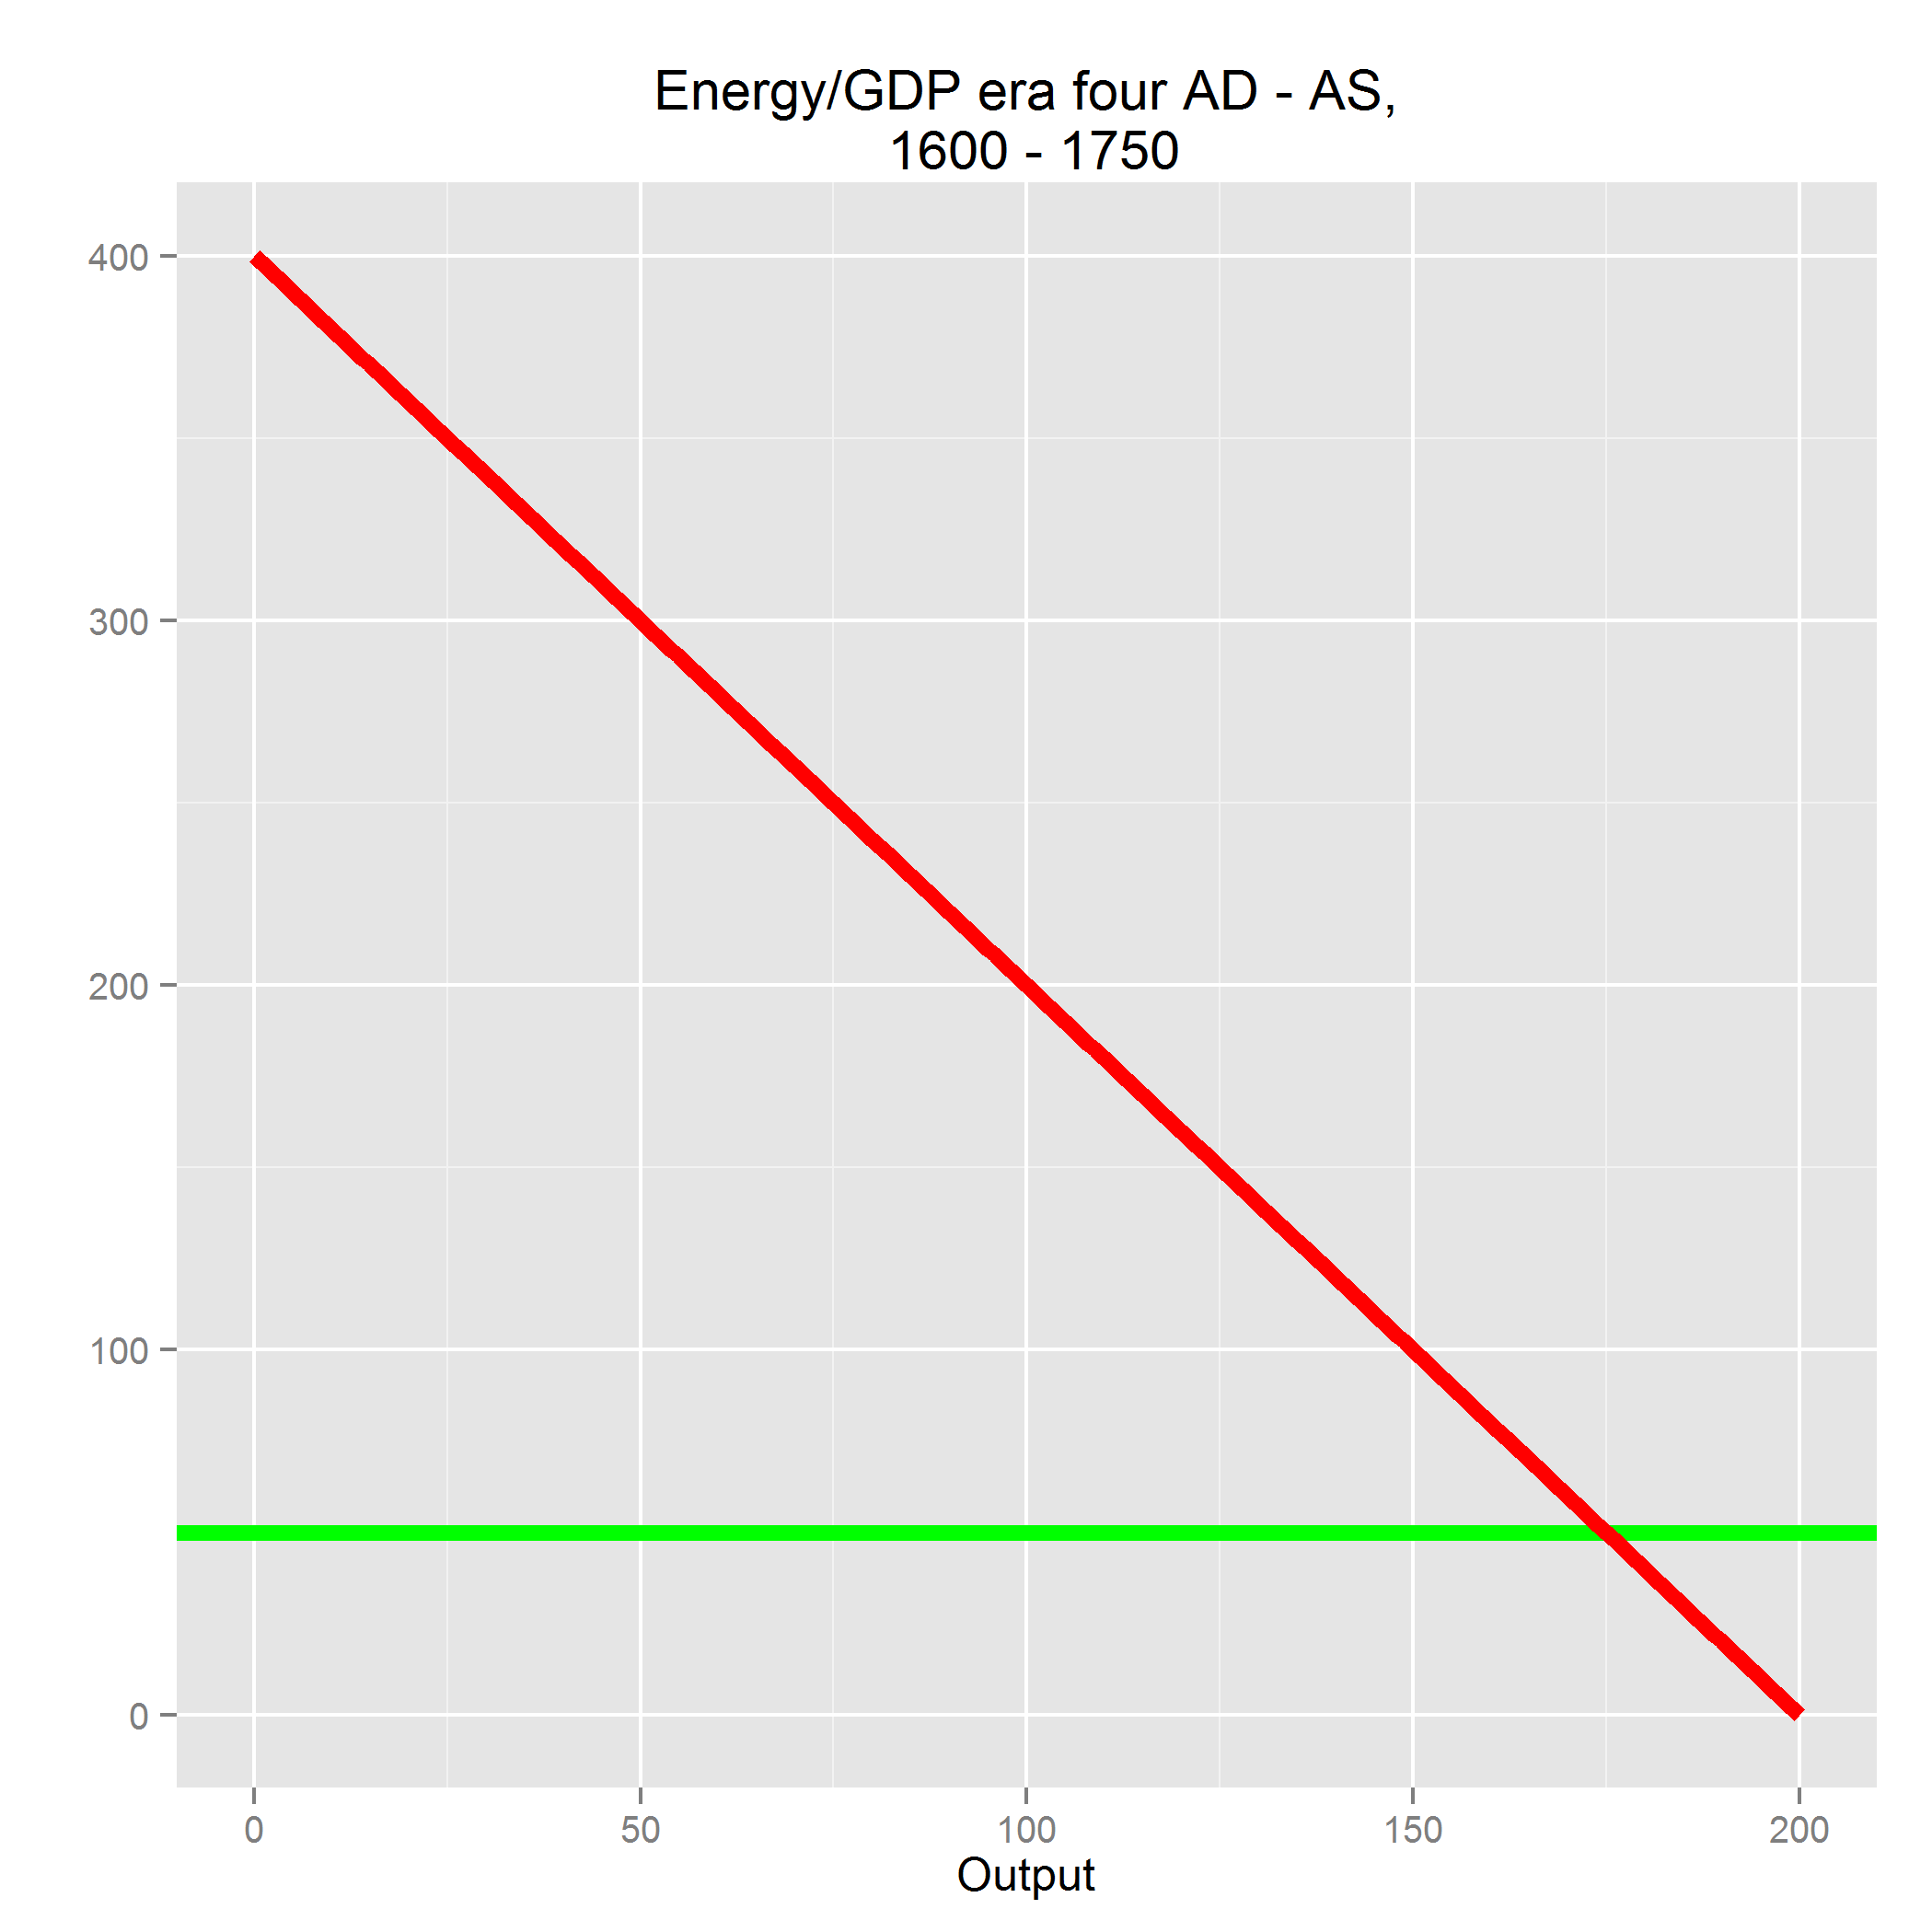
\includegraphics[height=0.5\textheight]{era4}}
		\mbox{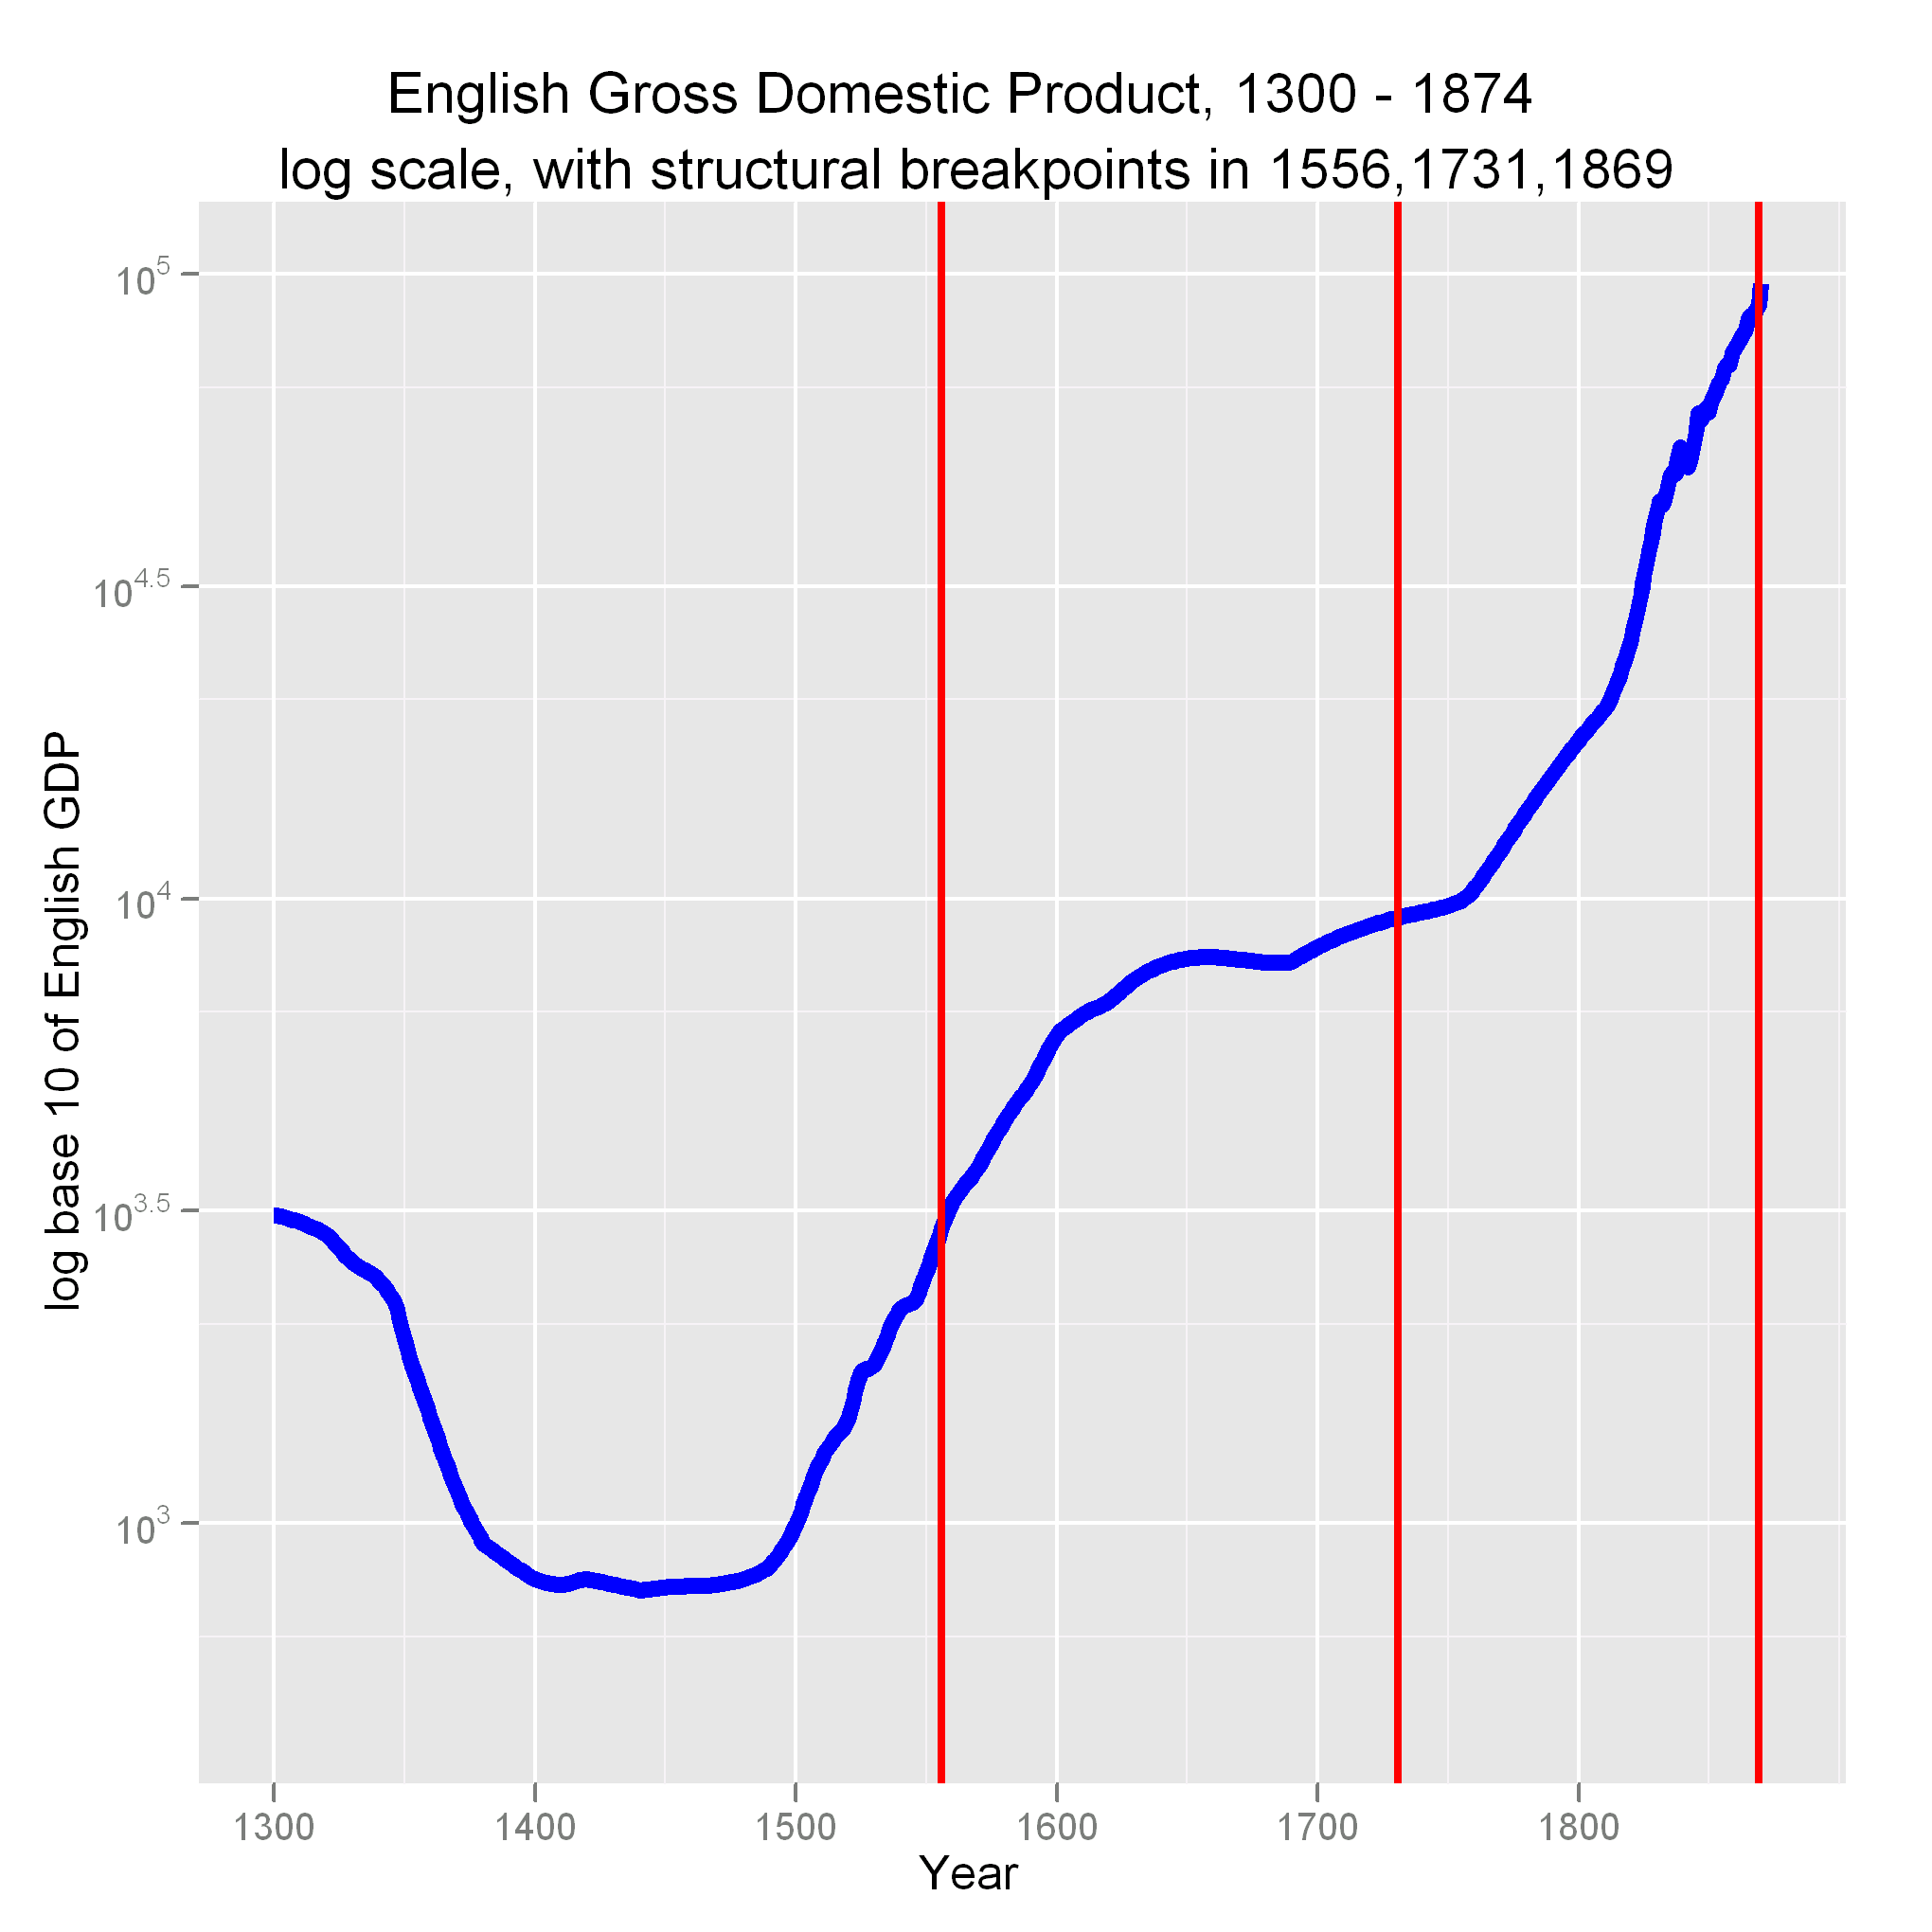
\includegraphics[height=0.5\textheight]{gbpgdplog}}
		\mbox{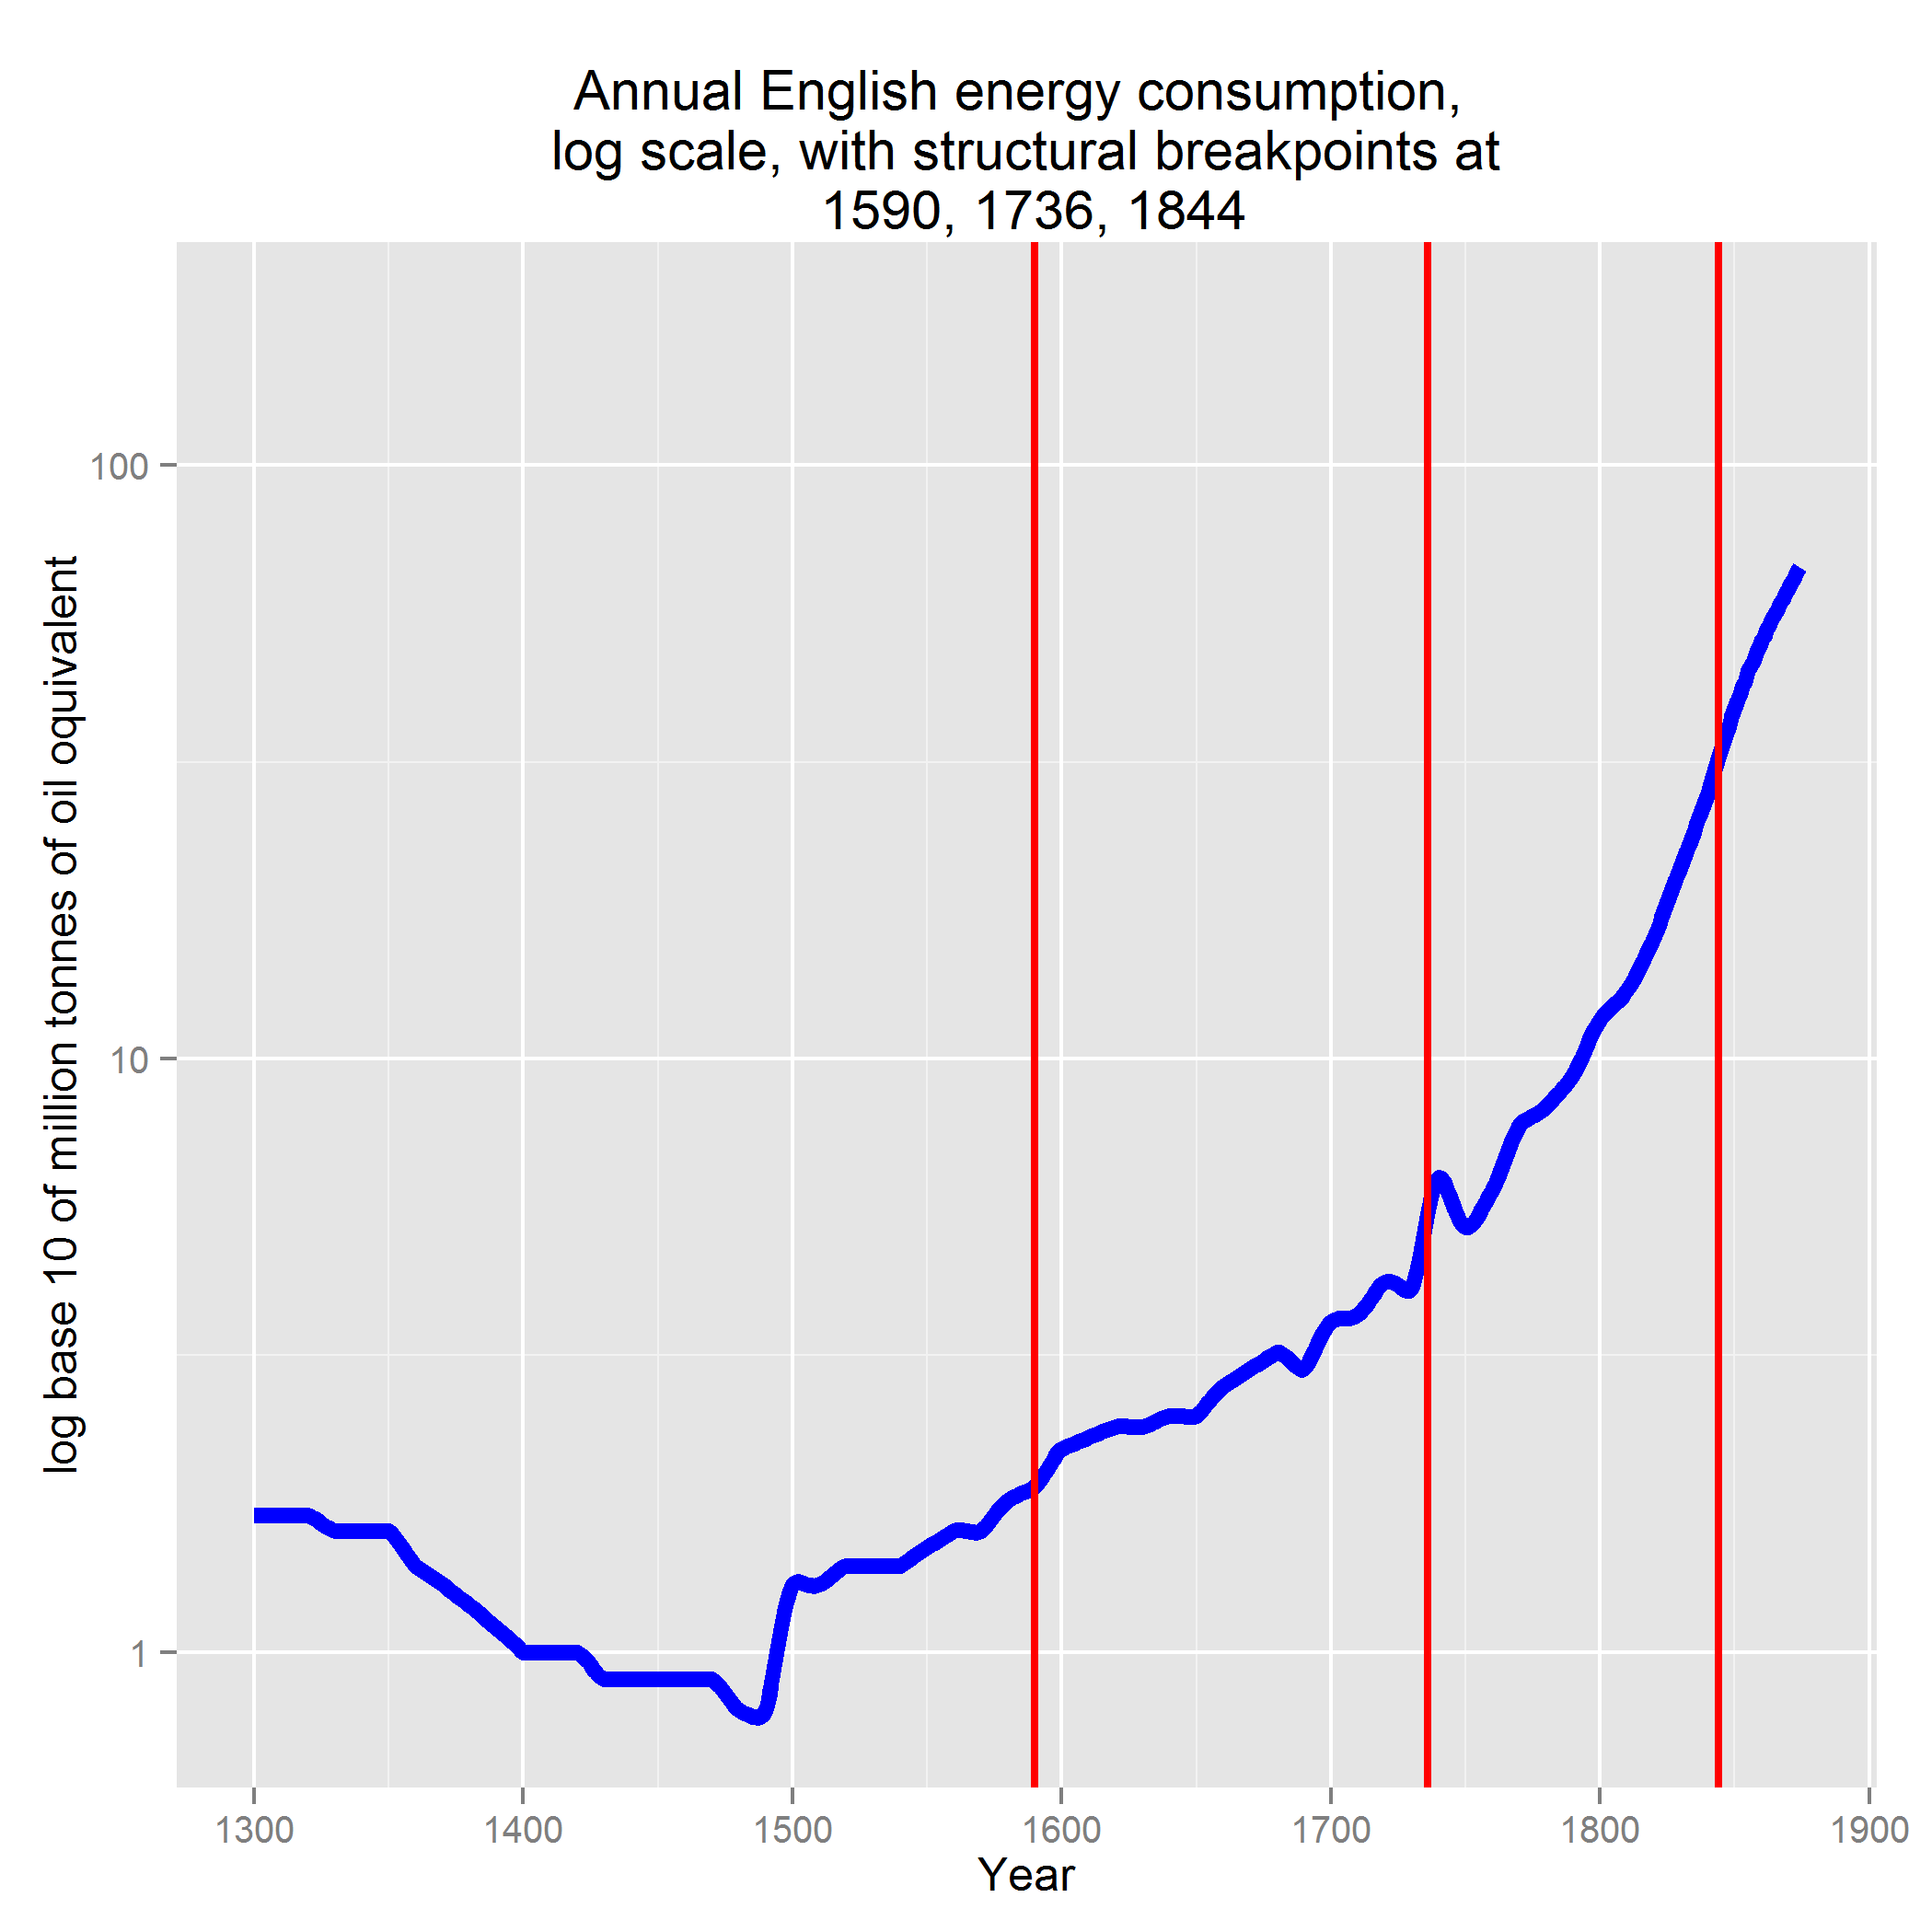
\includegraphics[height=0.5\textheight]{energyLog1}}
		}
		\end{figure} \vspace*{-0.4in}
Second energy revolution -- substitute steam power for labor power\\
Demand and supply expansion\\
Demand becomes the the system constraint\\
Modern economic growth\\
\end{frame}


\begin{frame}
		\frametitle{Desagulier manuscript}
\begin{figure}[p!]
%		\caption{Desagulier manuscript}
		\label{fig:desagulier}		
		\center
%		\mbox{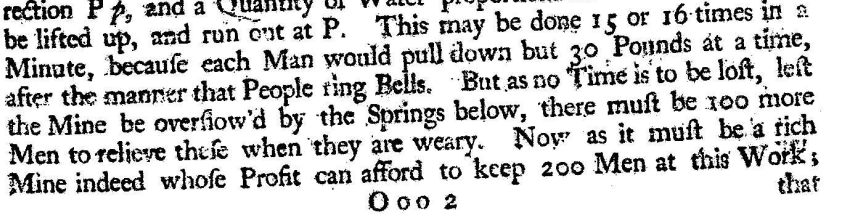
\includegraphics[width=0.95\textwidth]{desagulier1}}\\
%		\mbox{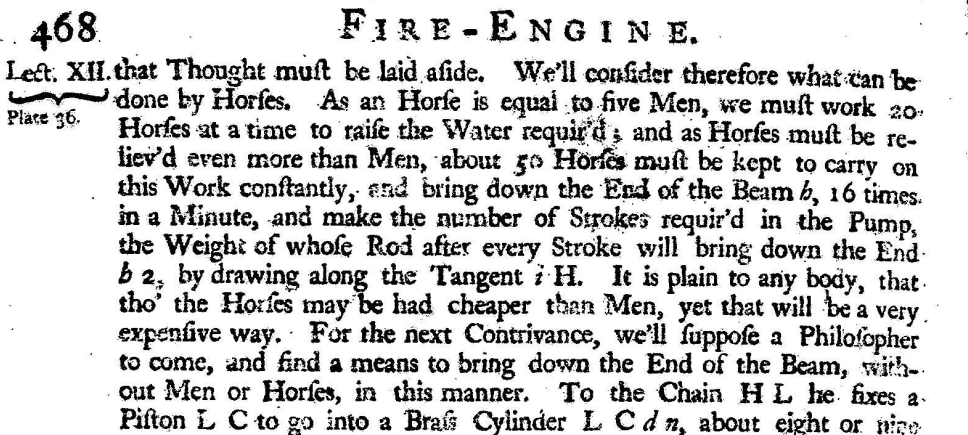
\includegraphics[width=0.95\textwidth]{desagulier2}}
		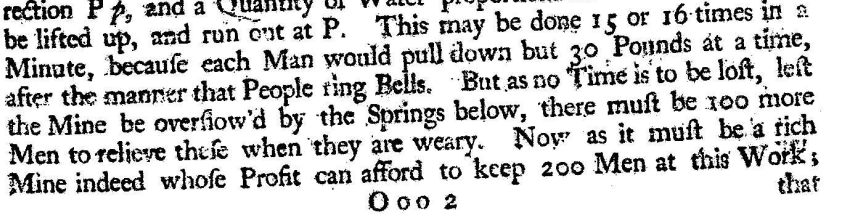
\includegraphics[width=0.95\textwidth]{desagulier1}\\
		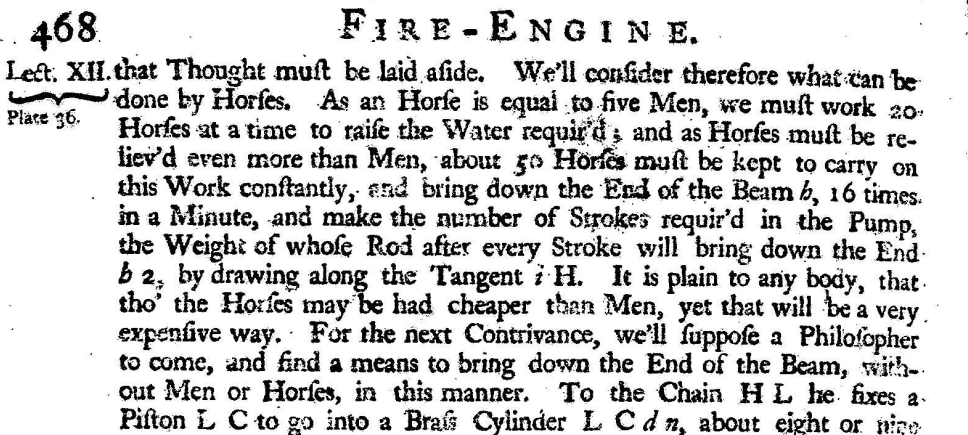
\includegraphics[width=1.05\textwidth]{desagulier2}
%		}
\end{figure}
\end{frame}


\begin{frame}
\frametitle{English real gross domestic product, \\
levels and per--capita }

		\begin{figure}[p!]
%		\caption{English real gross domestic product, \\
%		levels and per--capita }
		\label{fig:ggdp}		
		\centerline{
		\mbox{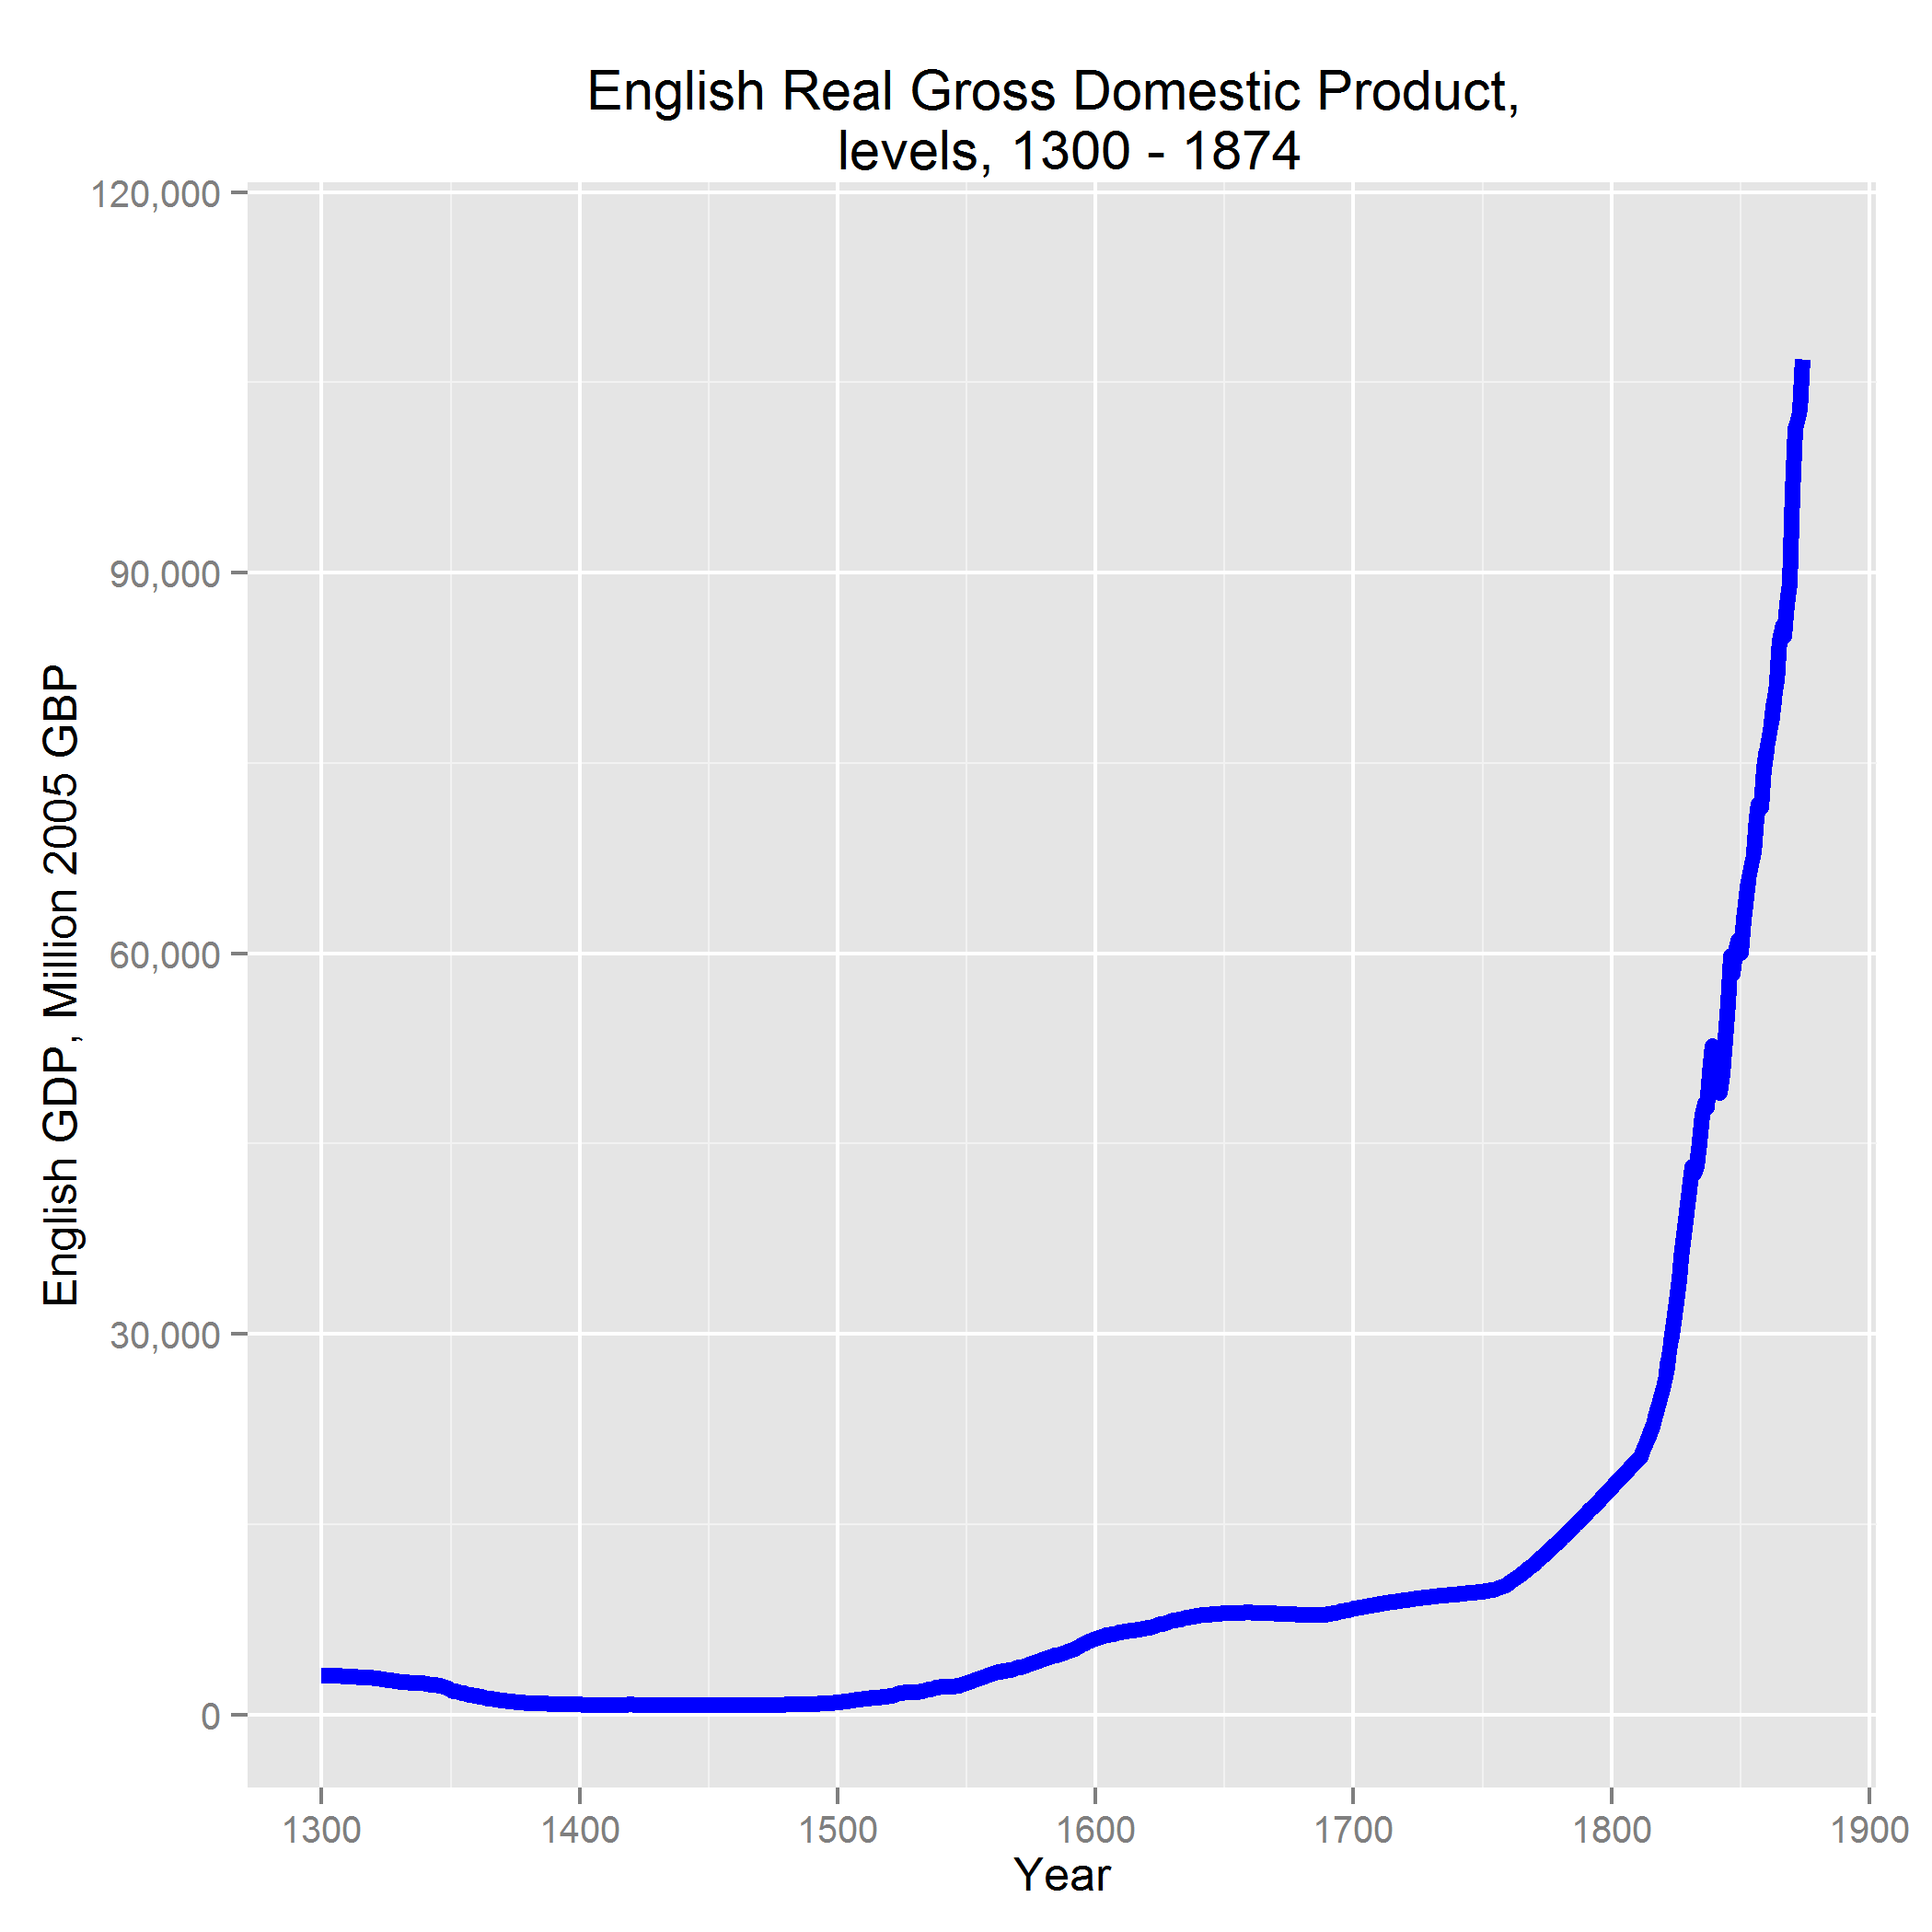
\includegraphics[width=0.55\textwidth]{ggdp}}
		\mbox{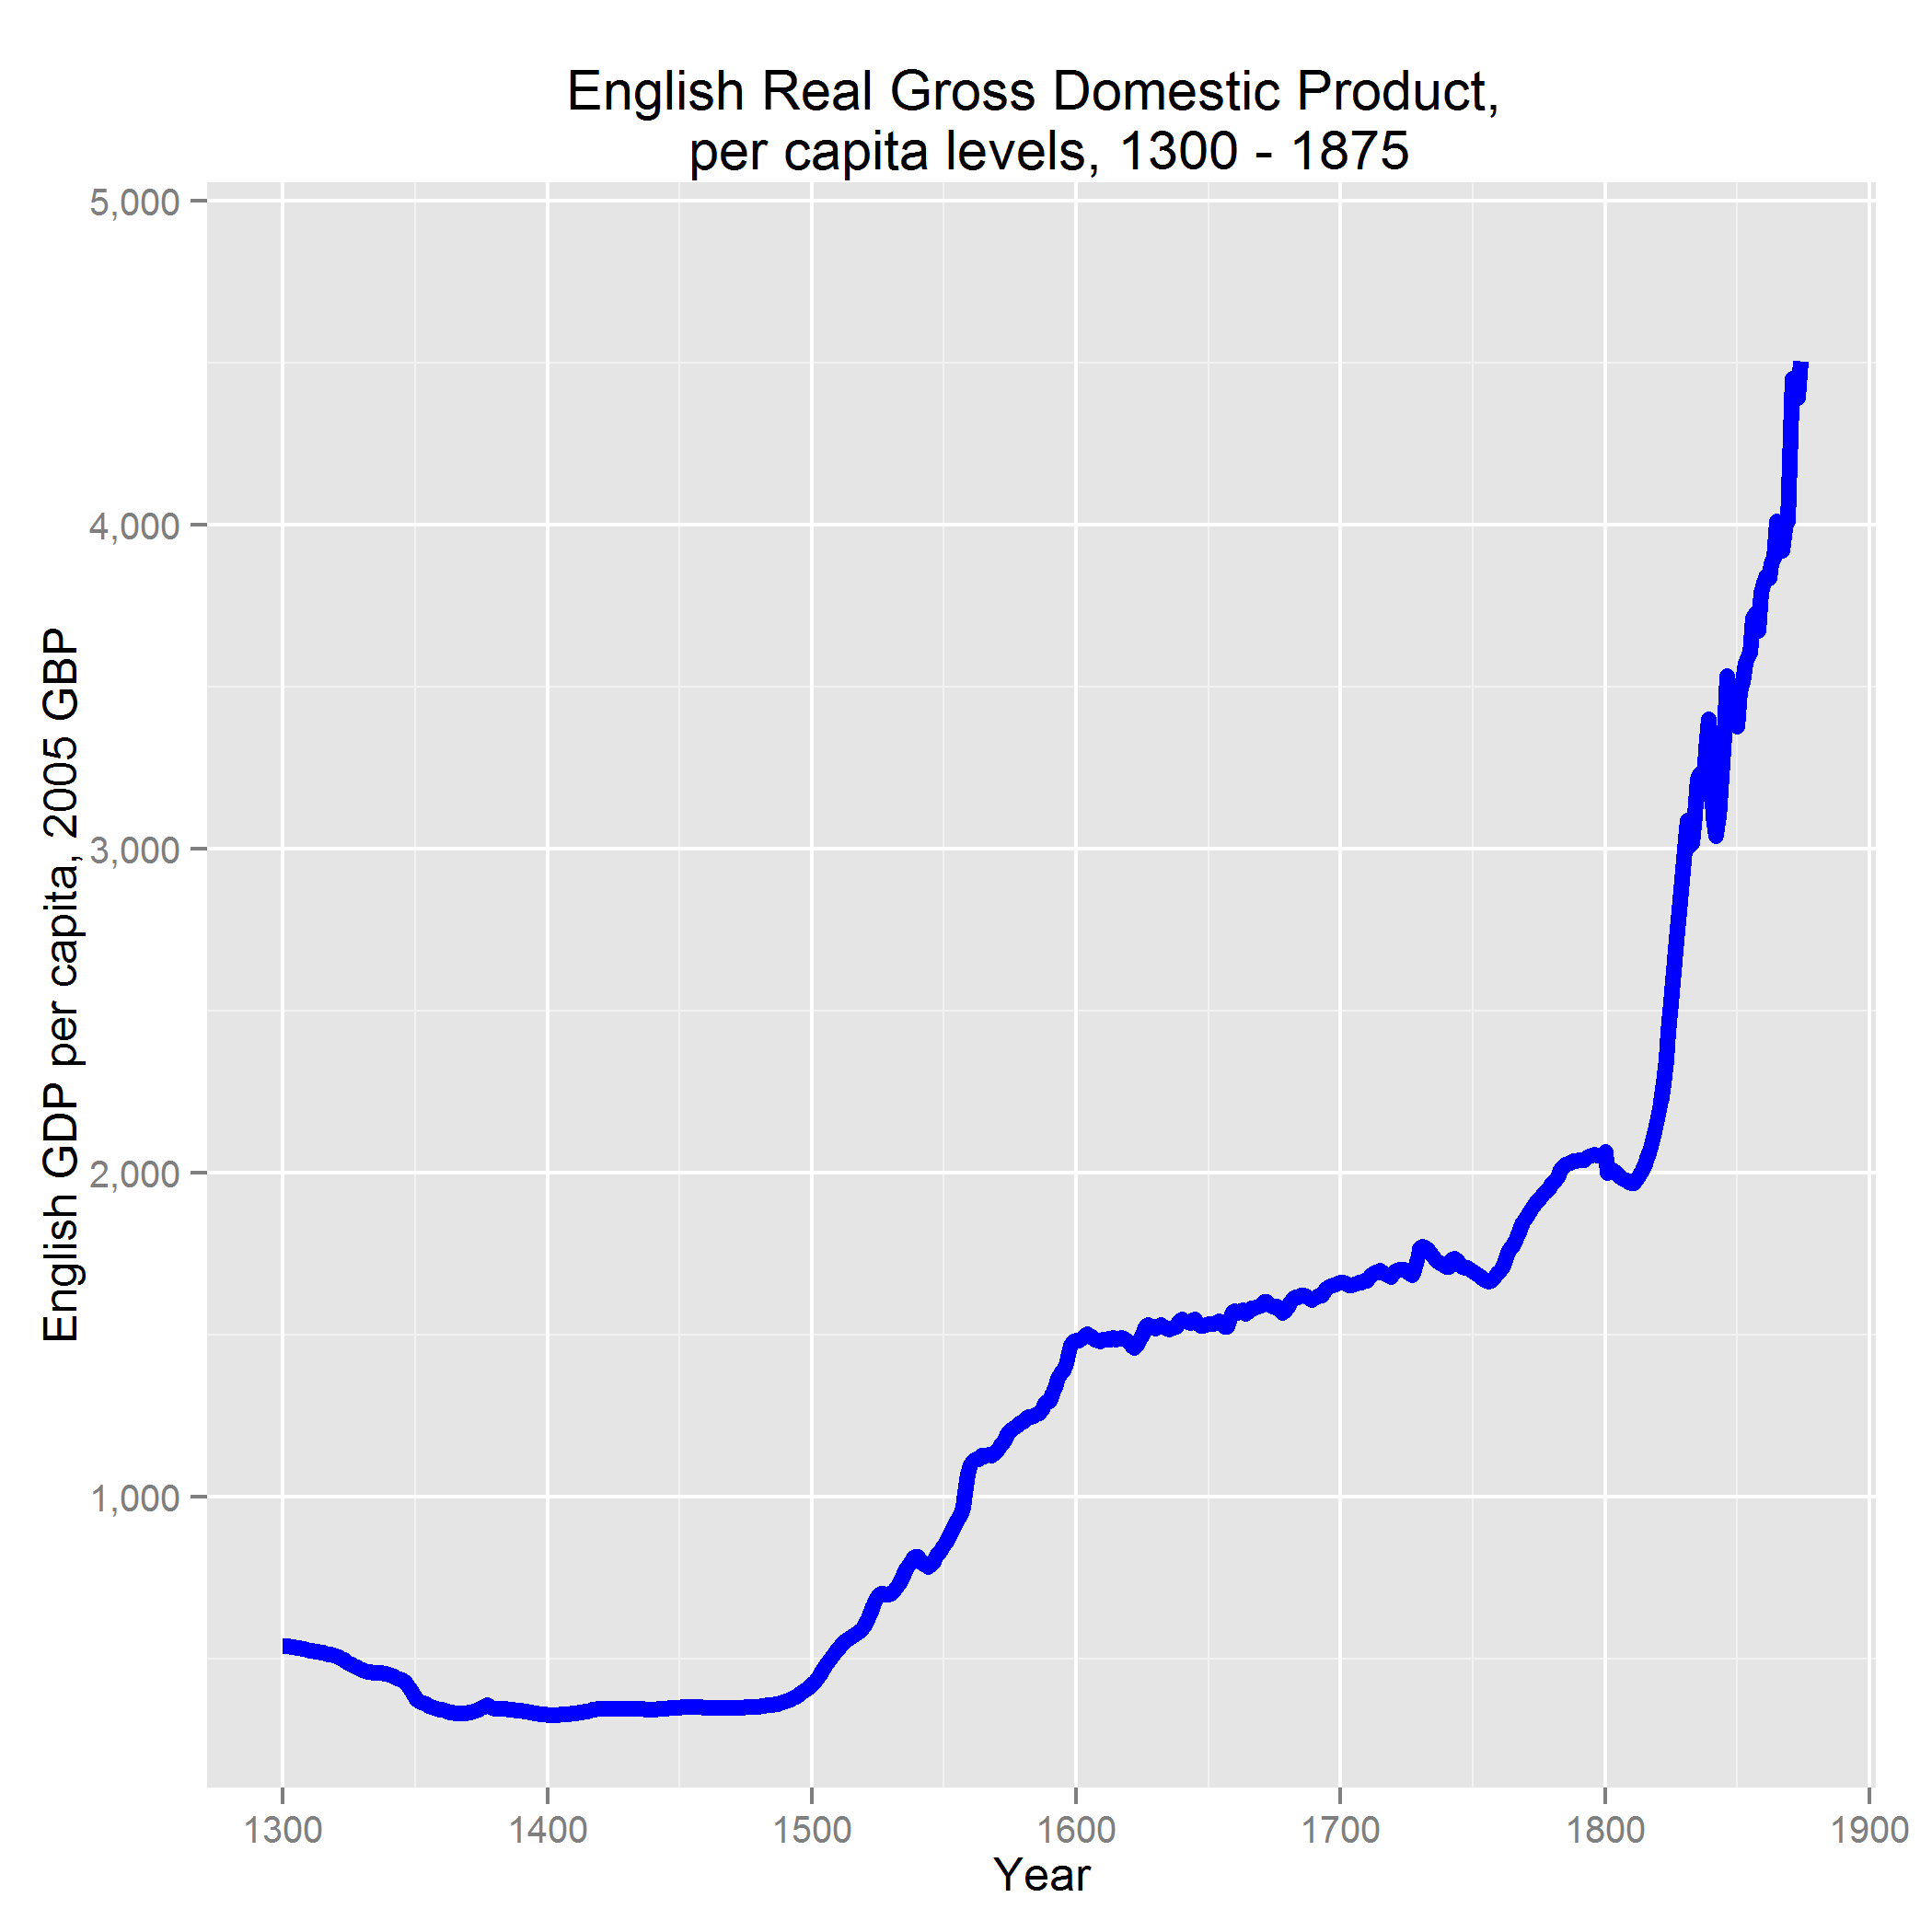
\includegraphics[width=0.55\textwidth]{ggdppop}}
		}
		\end{figure}
\end{frame}

\begin{frame}
		\frametitle{English real gross domestic product, \\
	log levels and log per--capita}

		\begin{figure}[p!]
%		\caption{English real gross domestic product, \\
%		log levels and log per--capita}
		\label{fig:gdpLog}		
		\centerline{
		\mbox{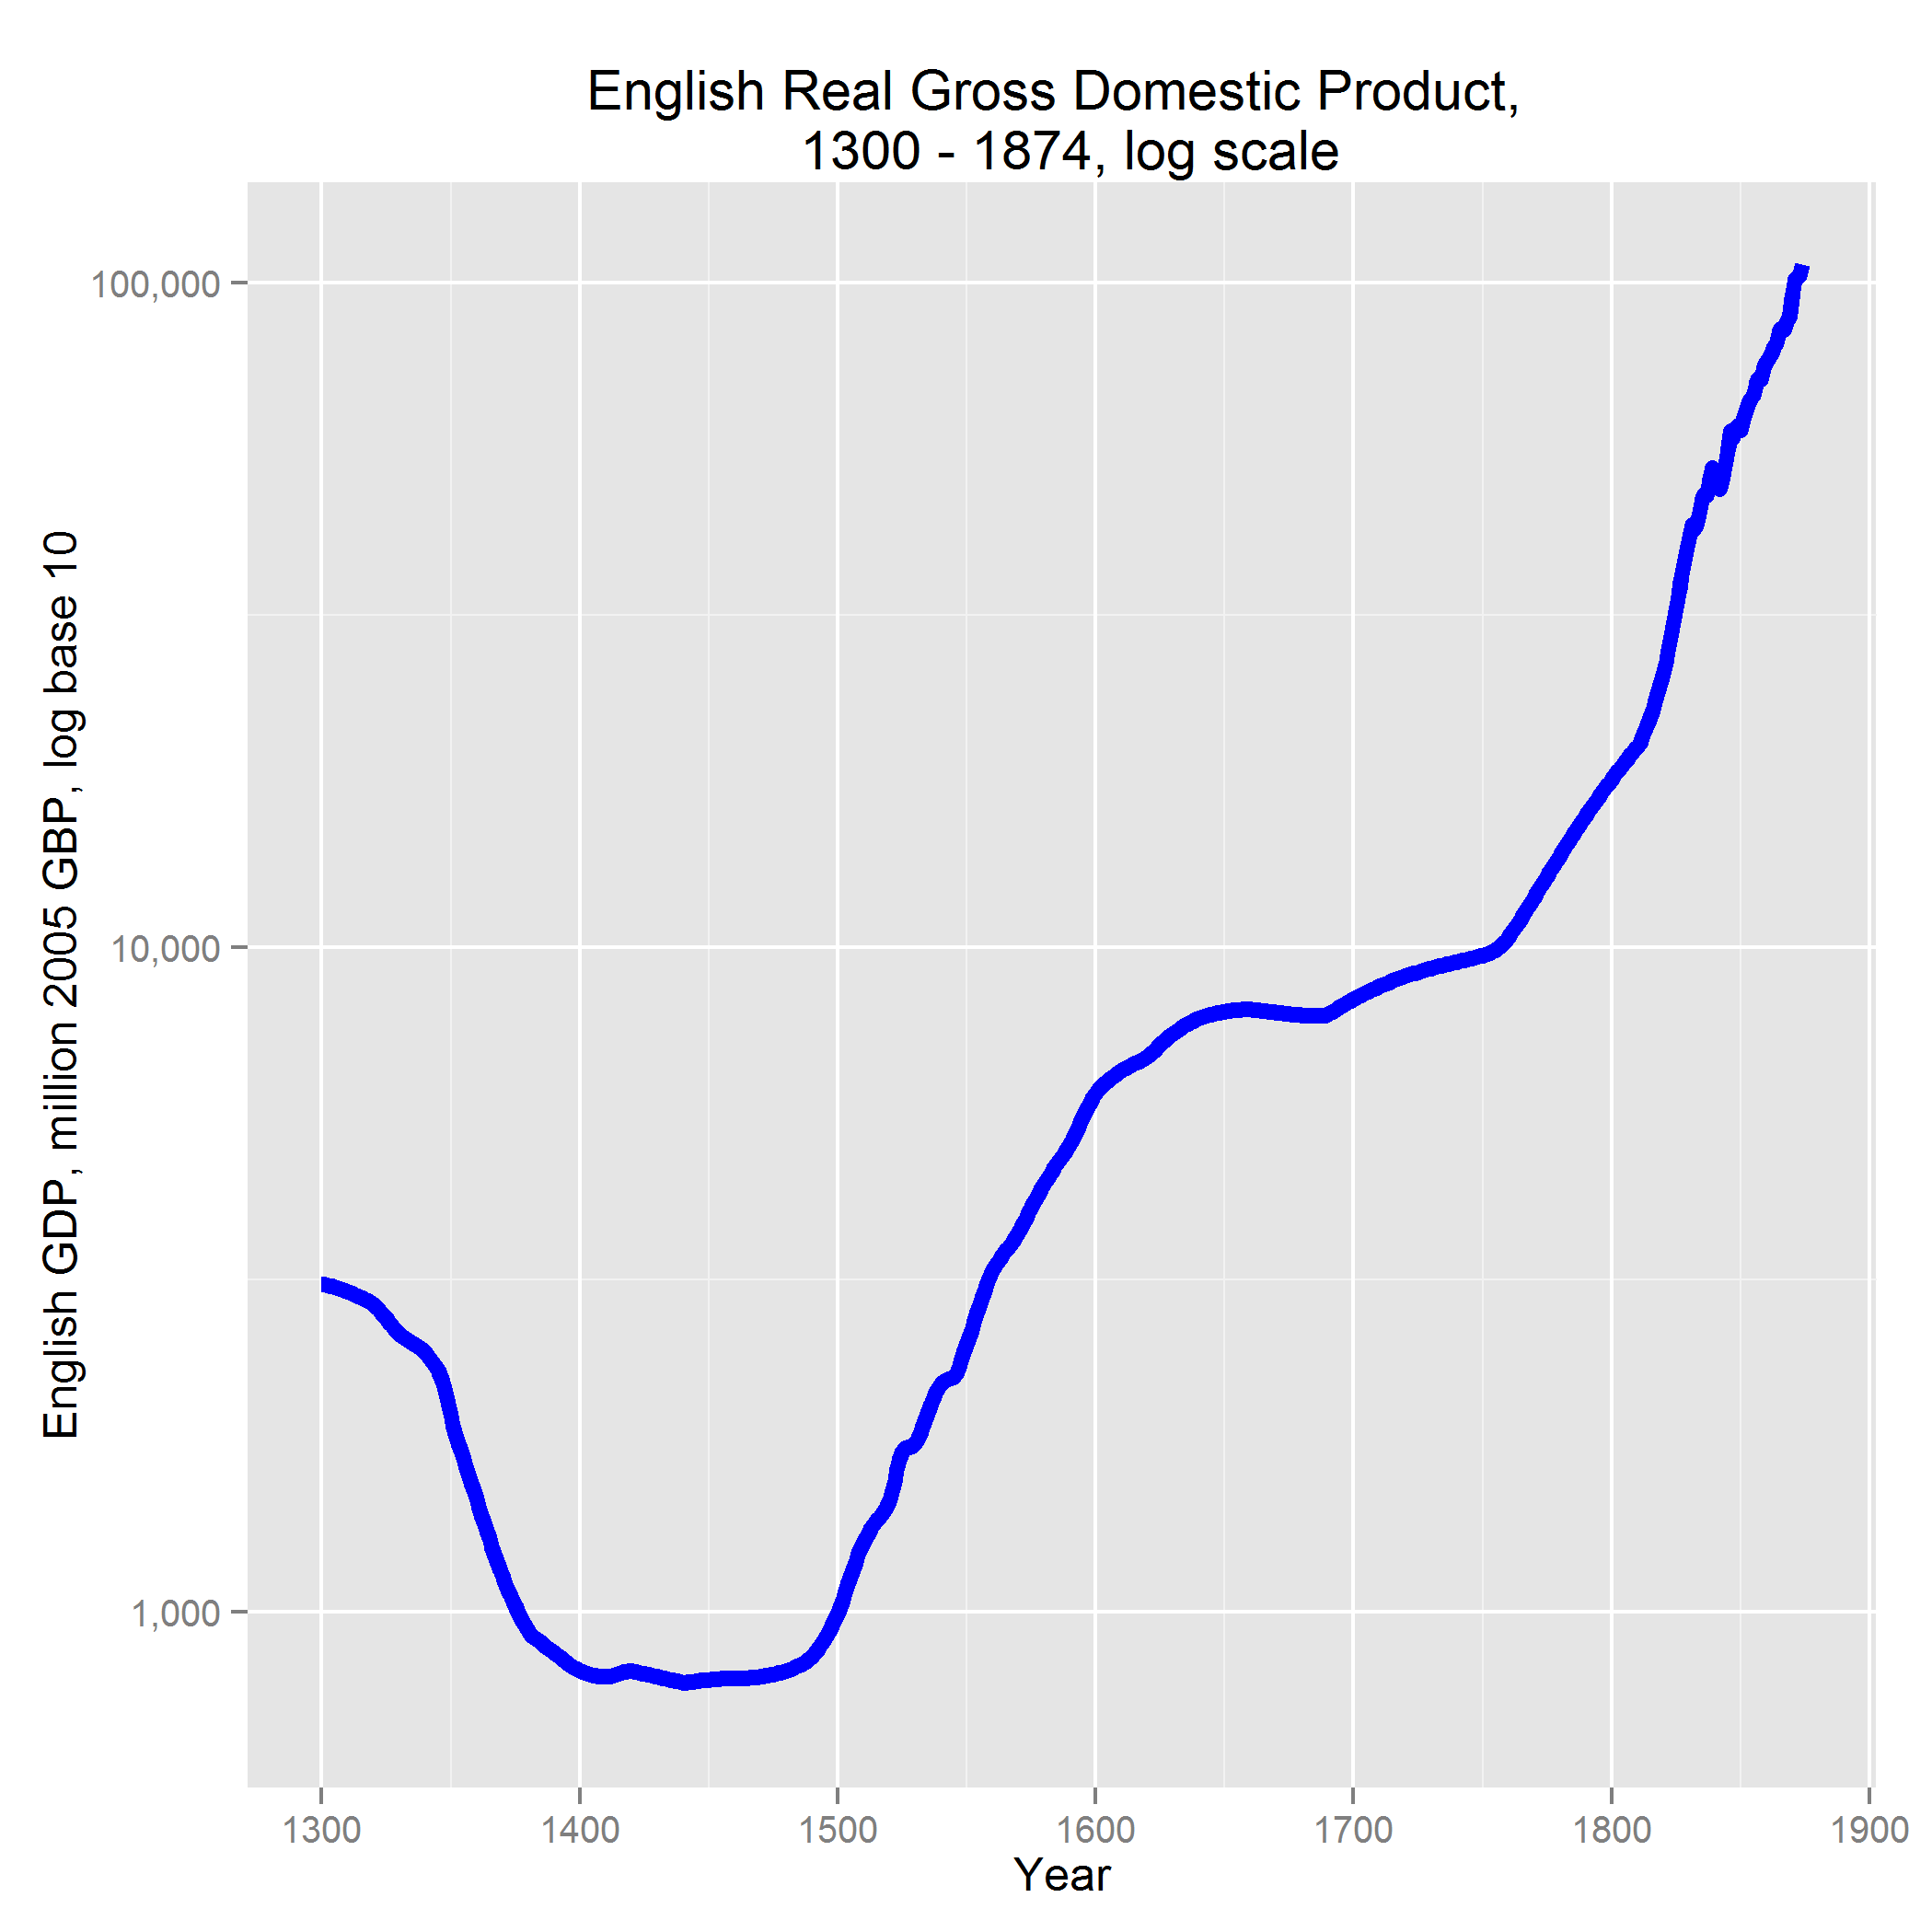
\includegraphics[width=0.55\textwidth]{gdpLog}}
		\mbox{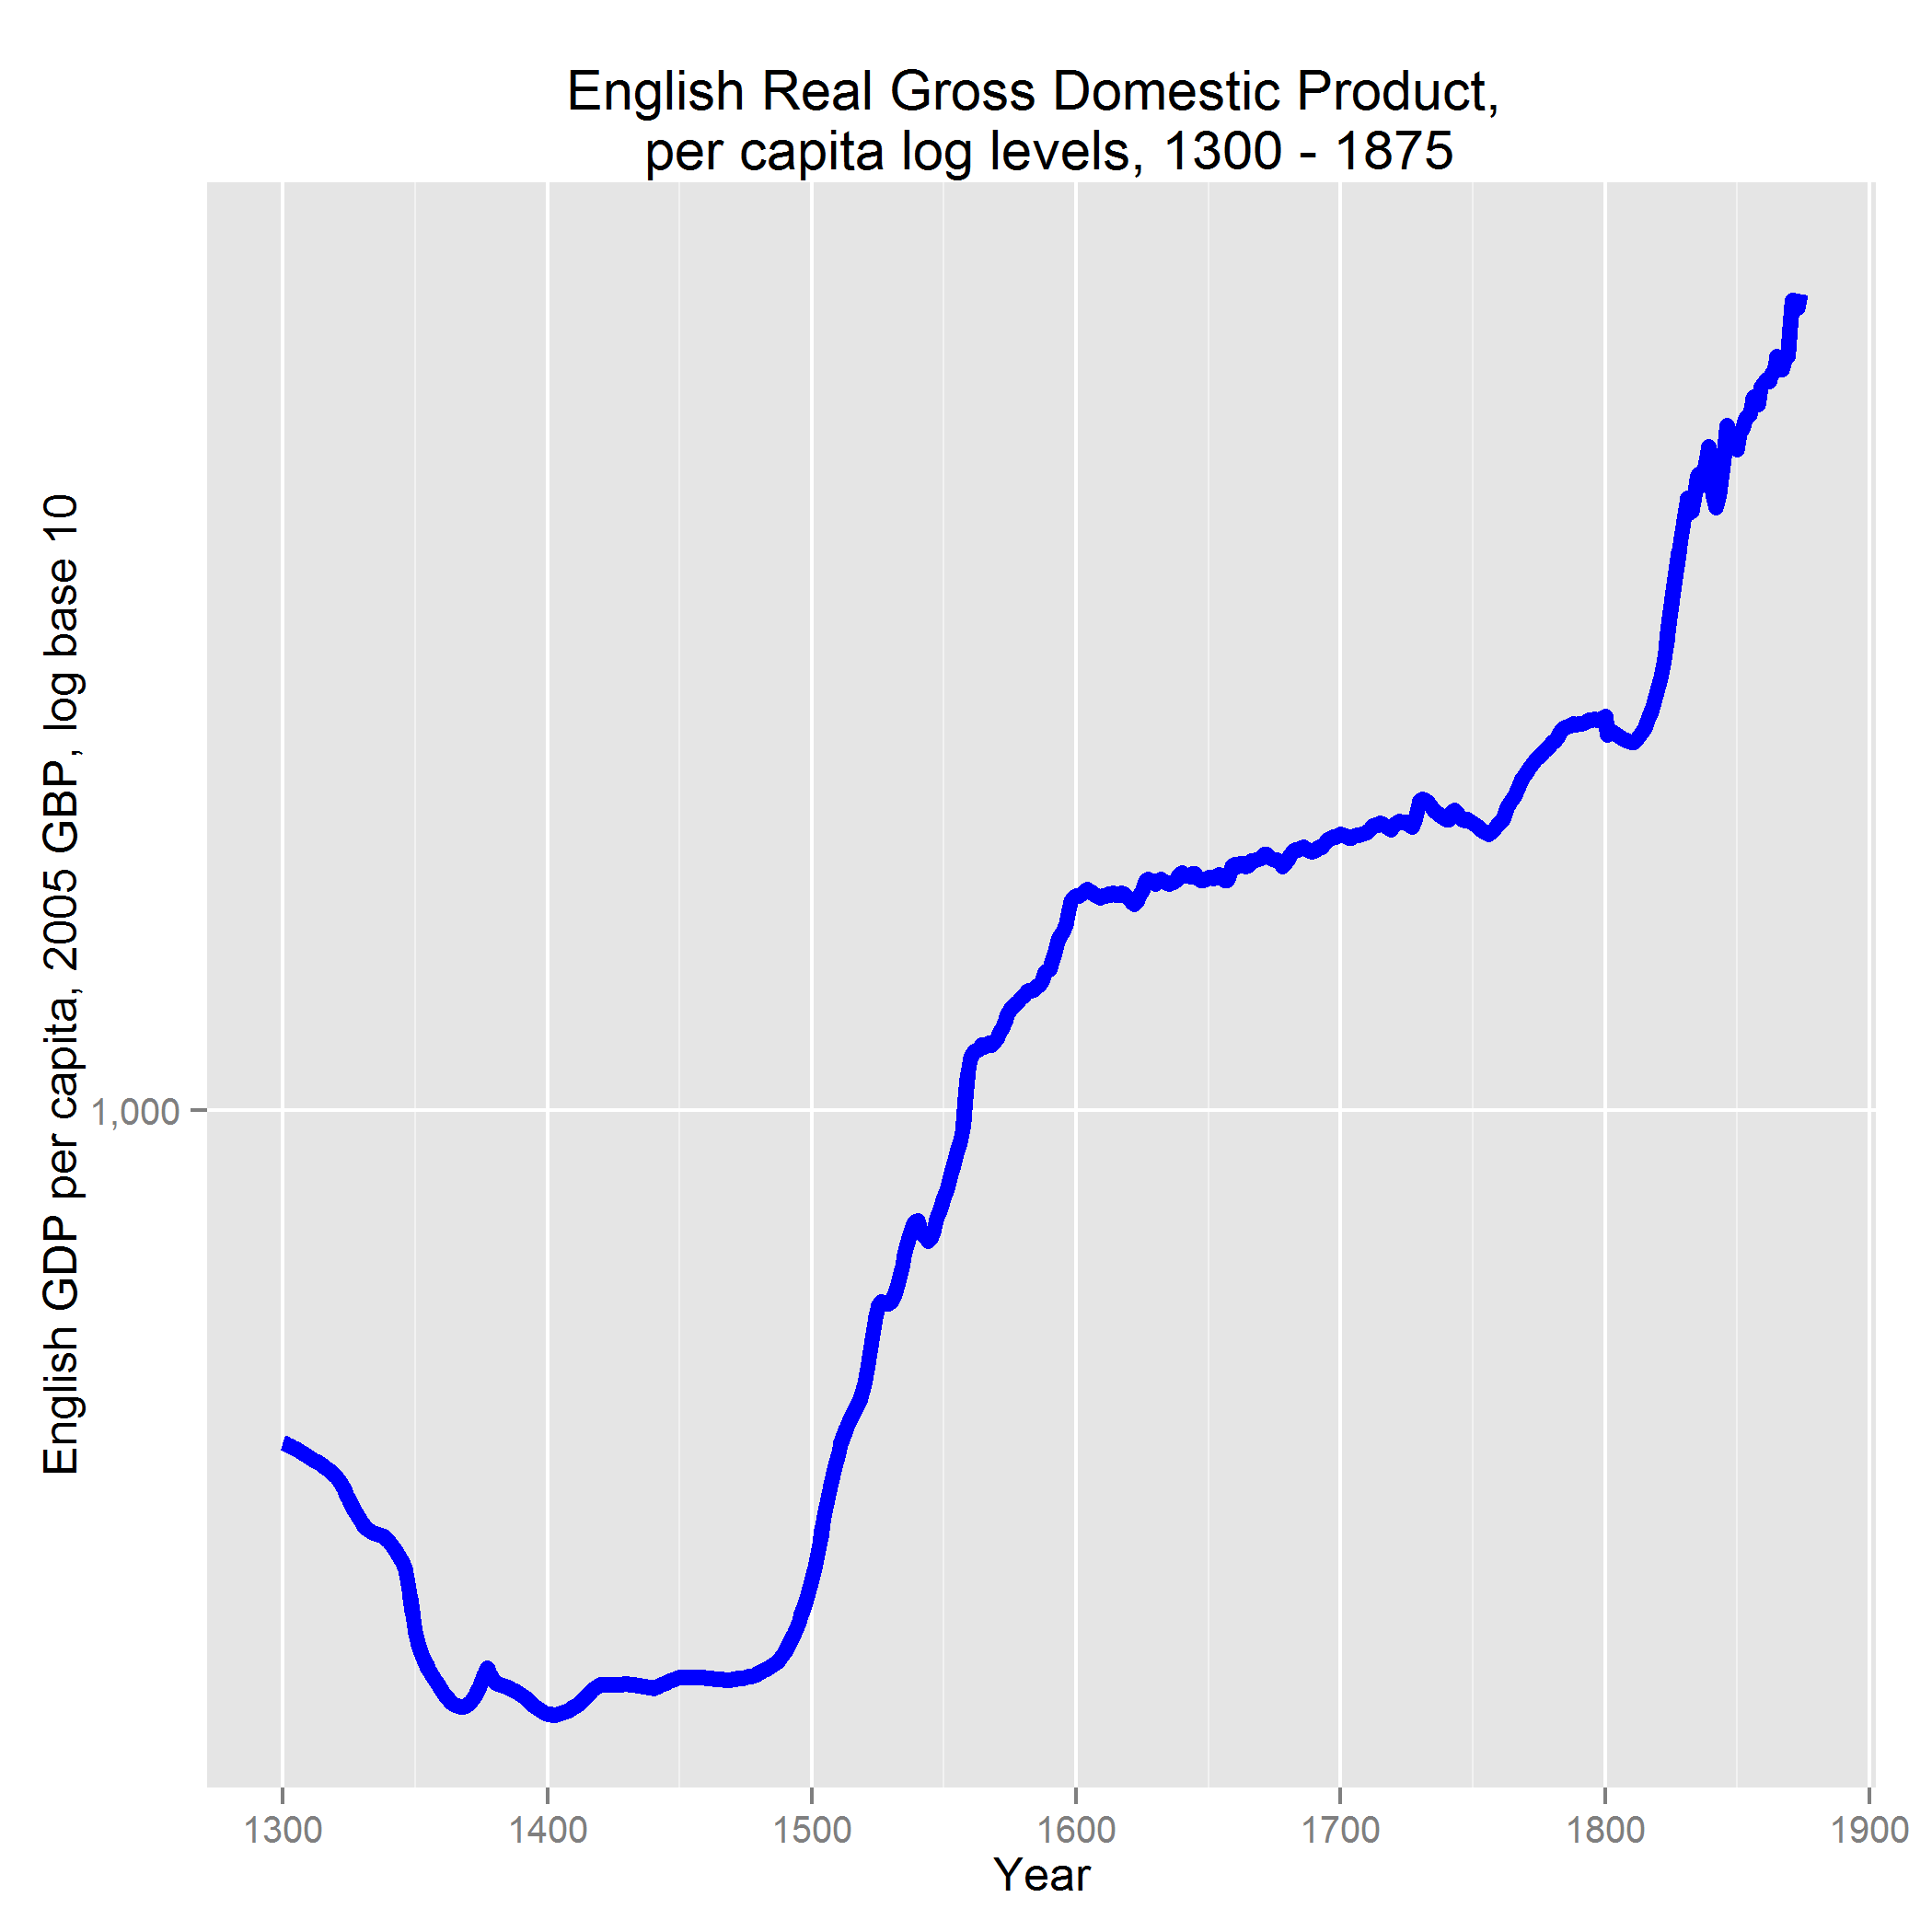
\includegraphics[width=0.55\textwidth]{gdpPopLog}}
		}
		\end{figure}
\end{frame}

\begin{frame}
		\frametitle{Structural break comparison}
\begin{figure}[p!]
%		\caption{Structural break comparison}
		\label{fig:structural}		
		\centerline{
		\mbox{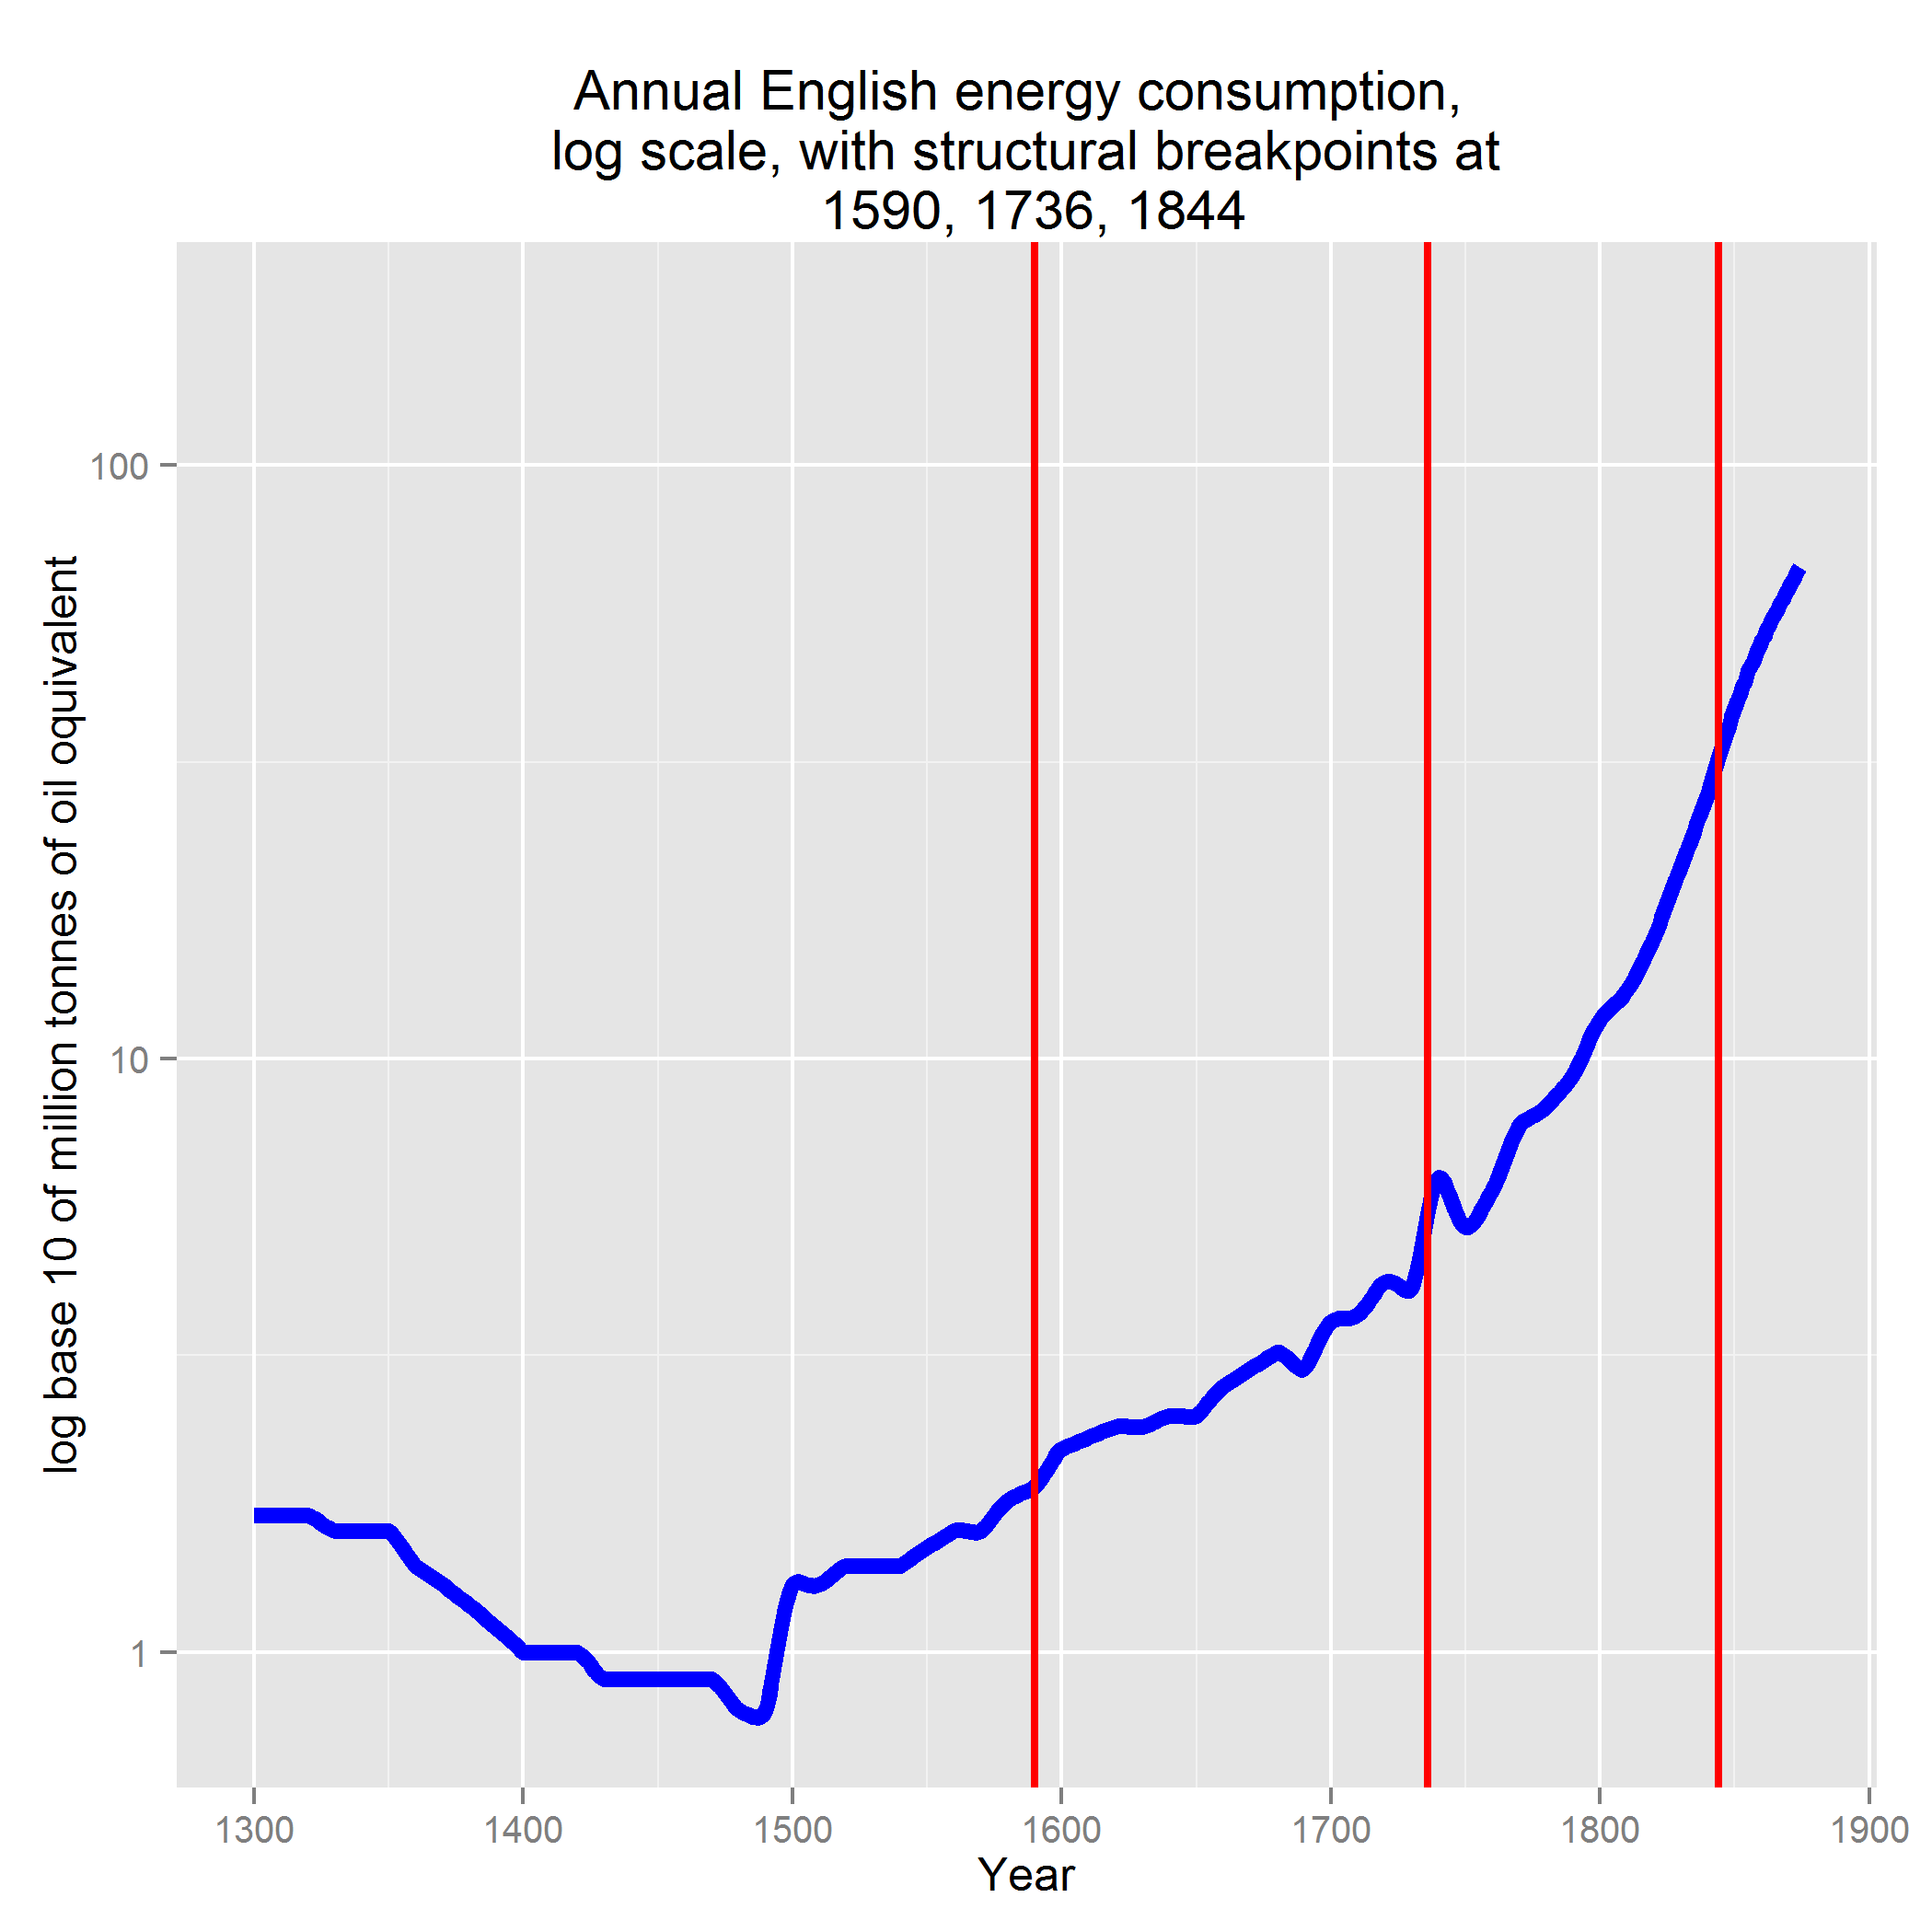
\includegraphics[width=0.39\textwidth]{energyLog1}}
		\mbox{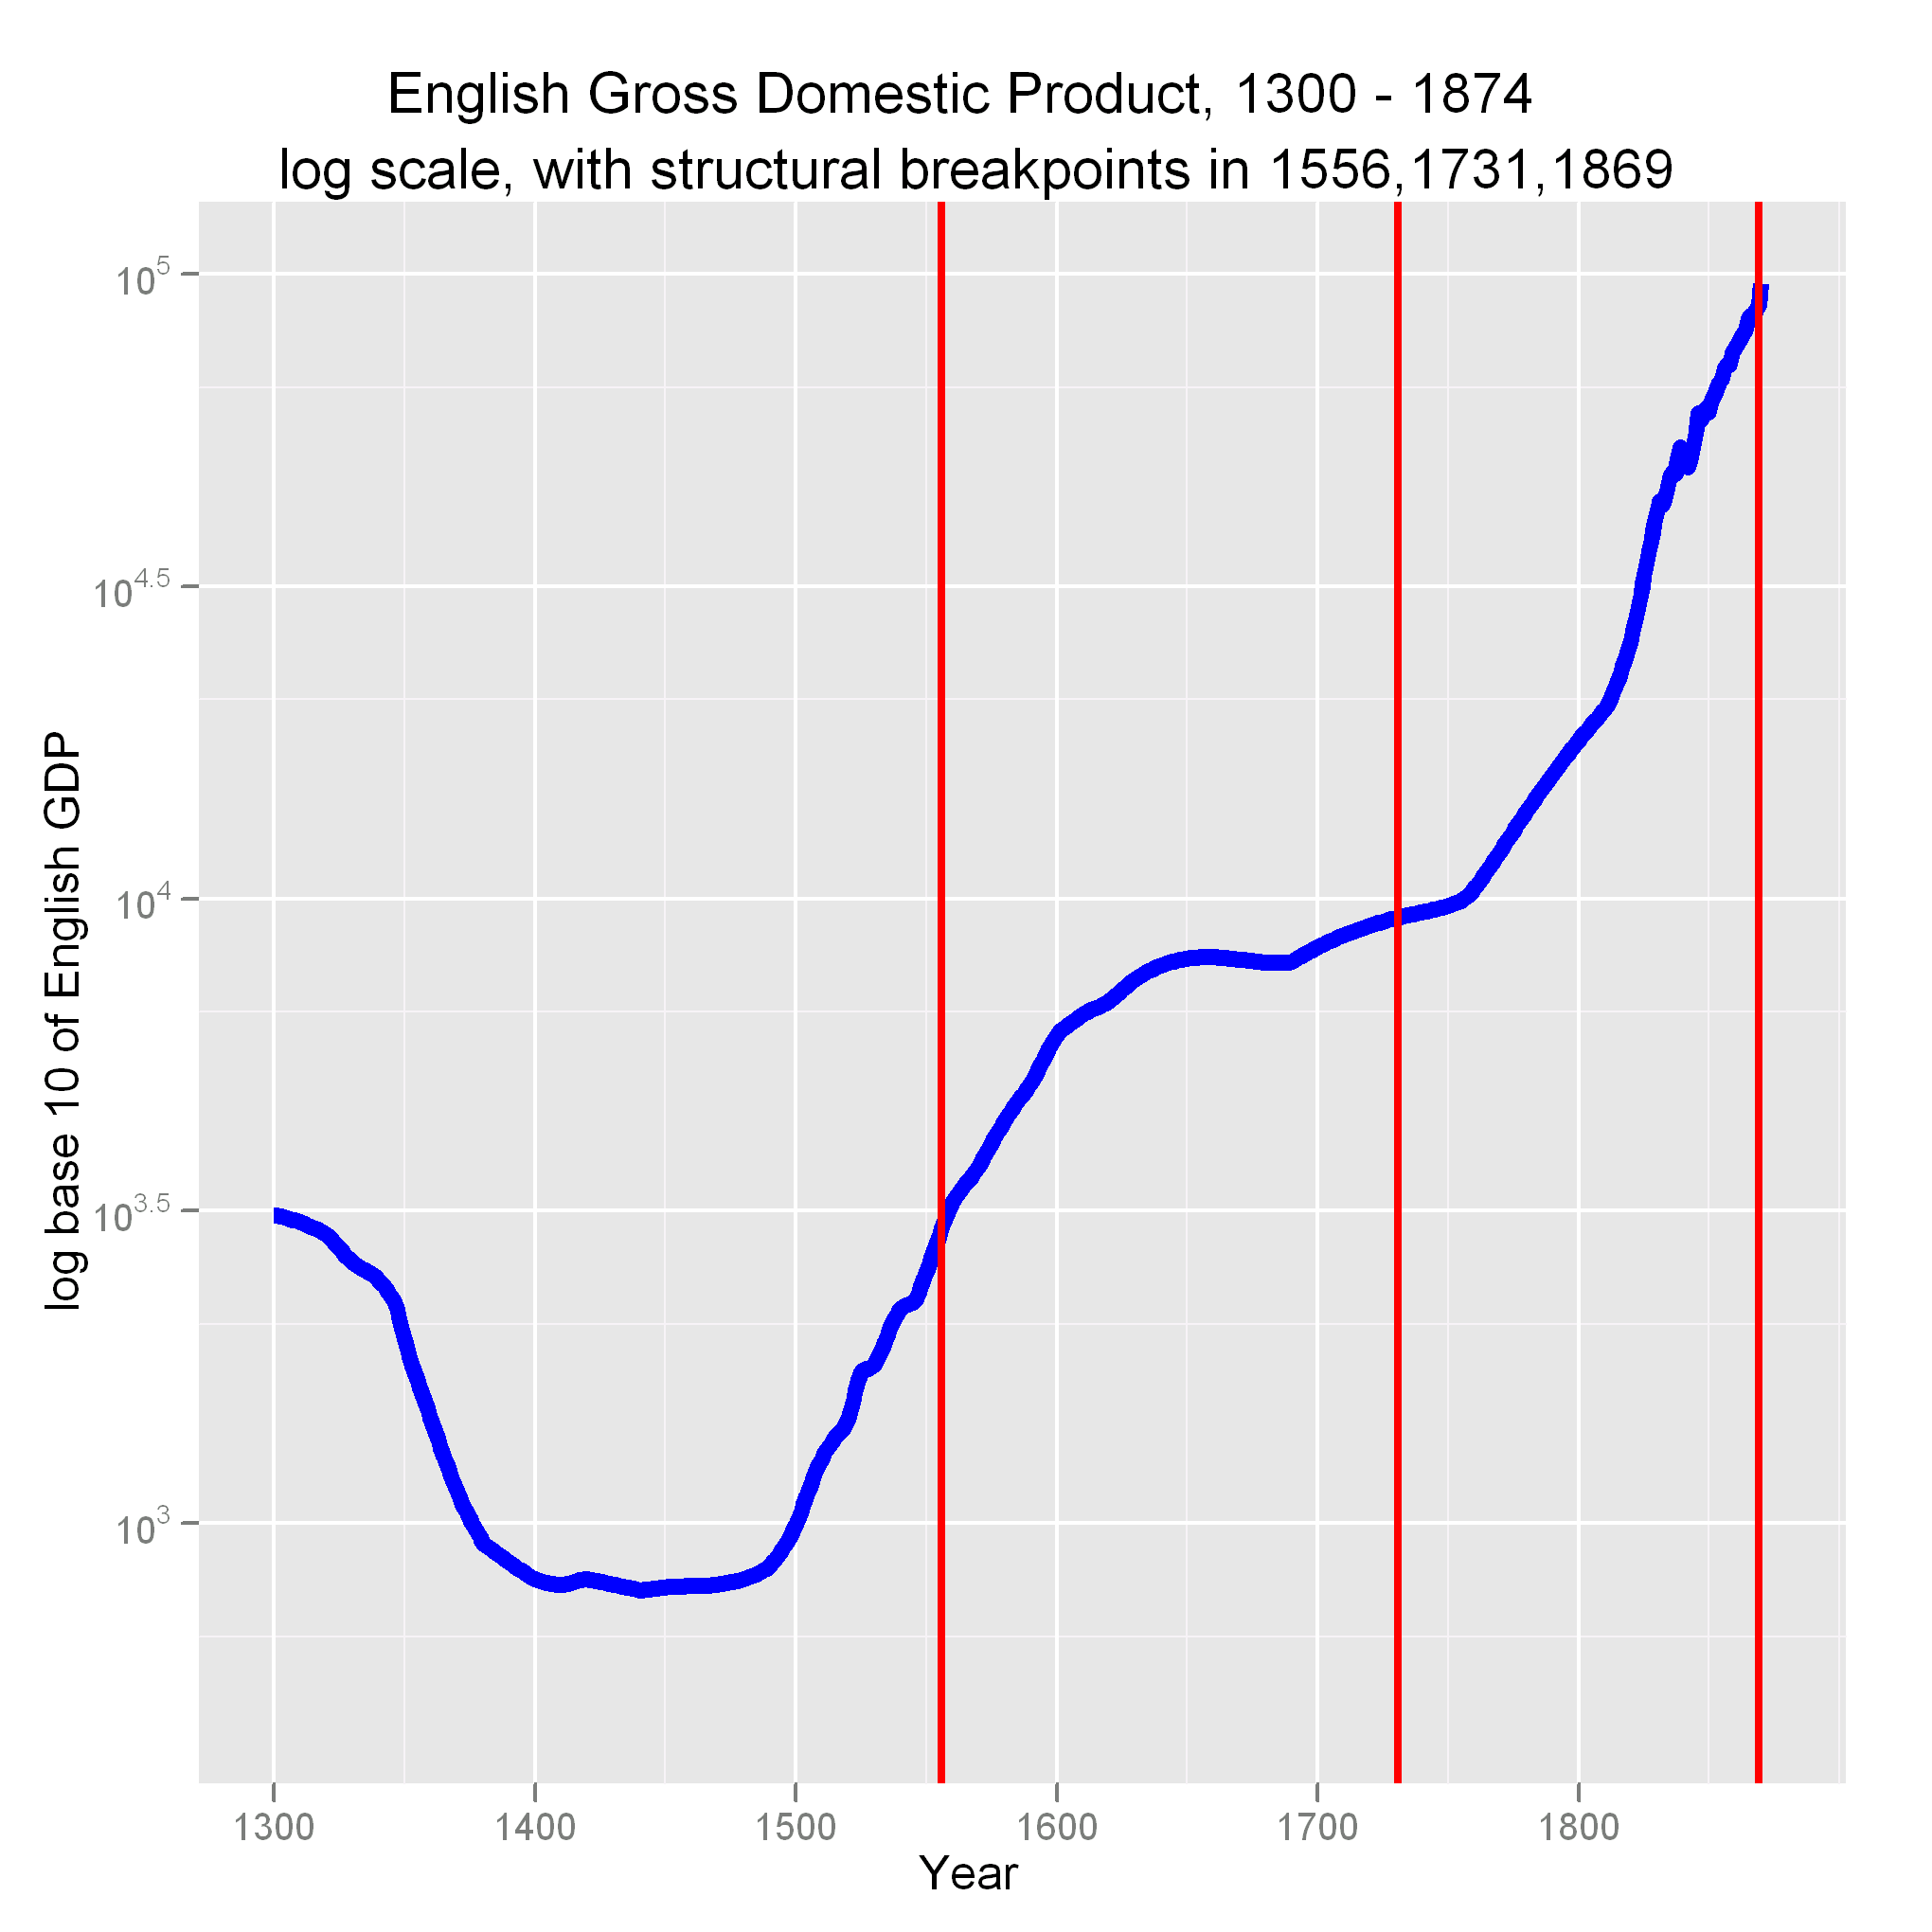
\includegraphics[width=0.39\textwidth]{gbpgdplog}}
		\mbox{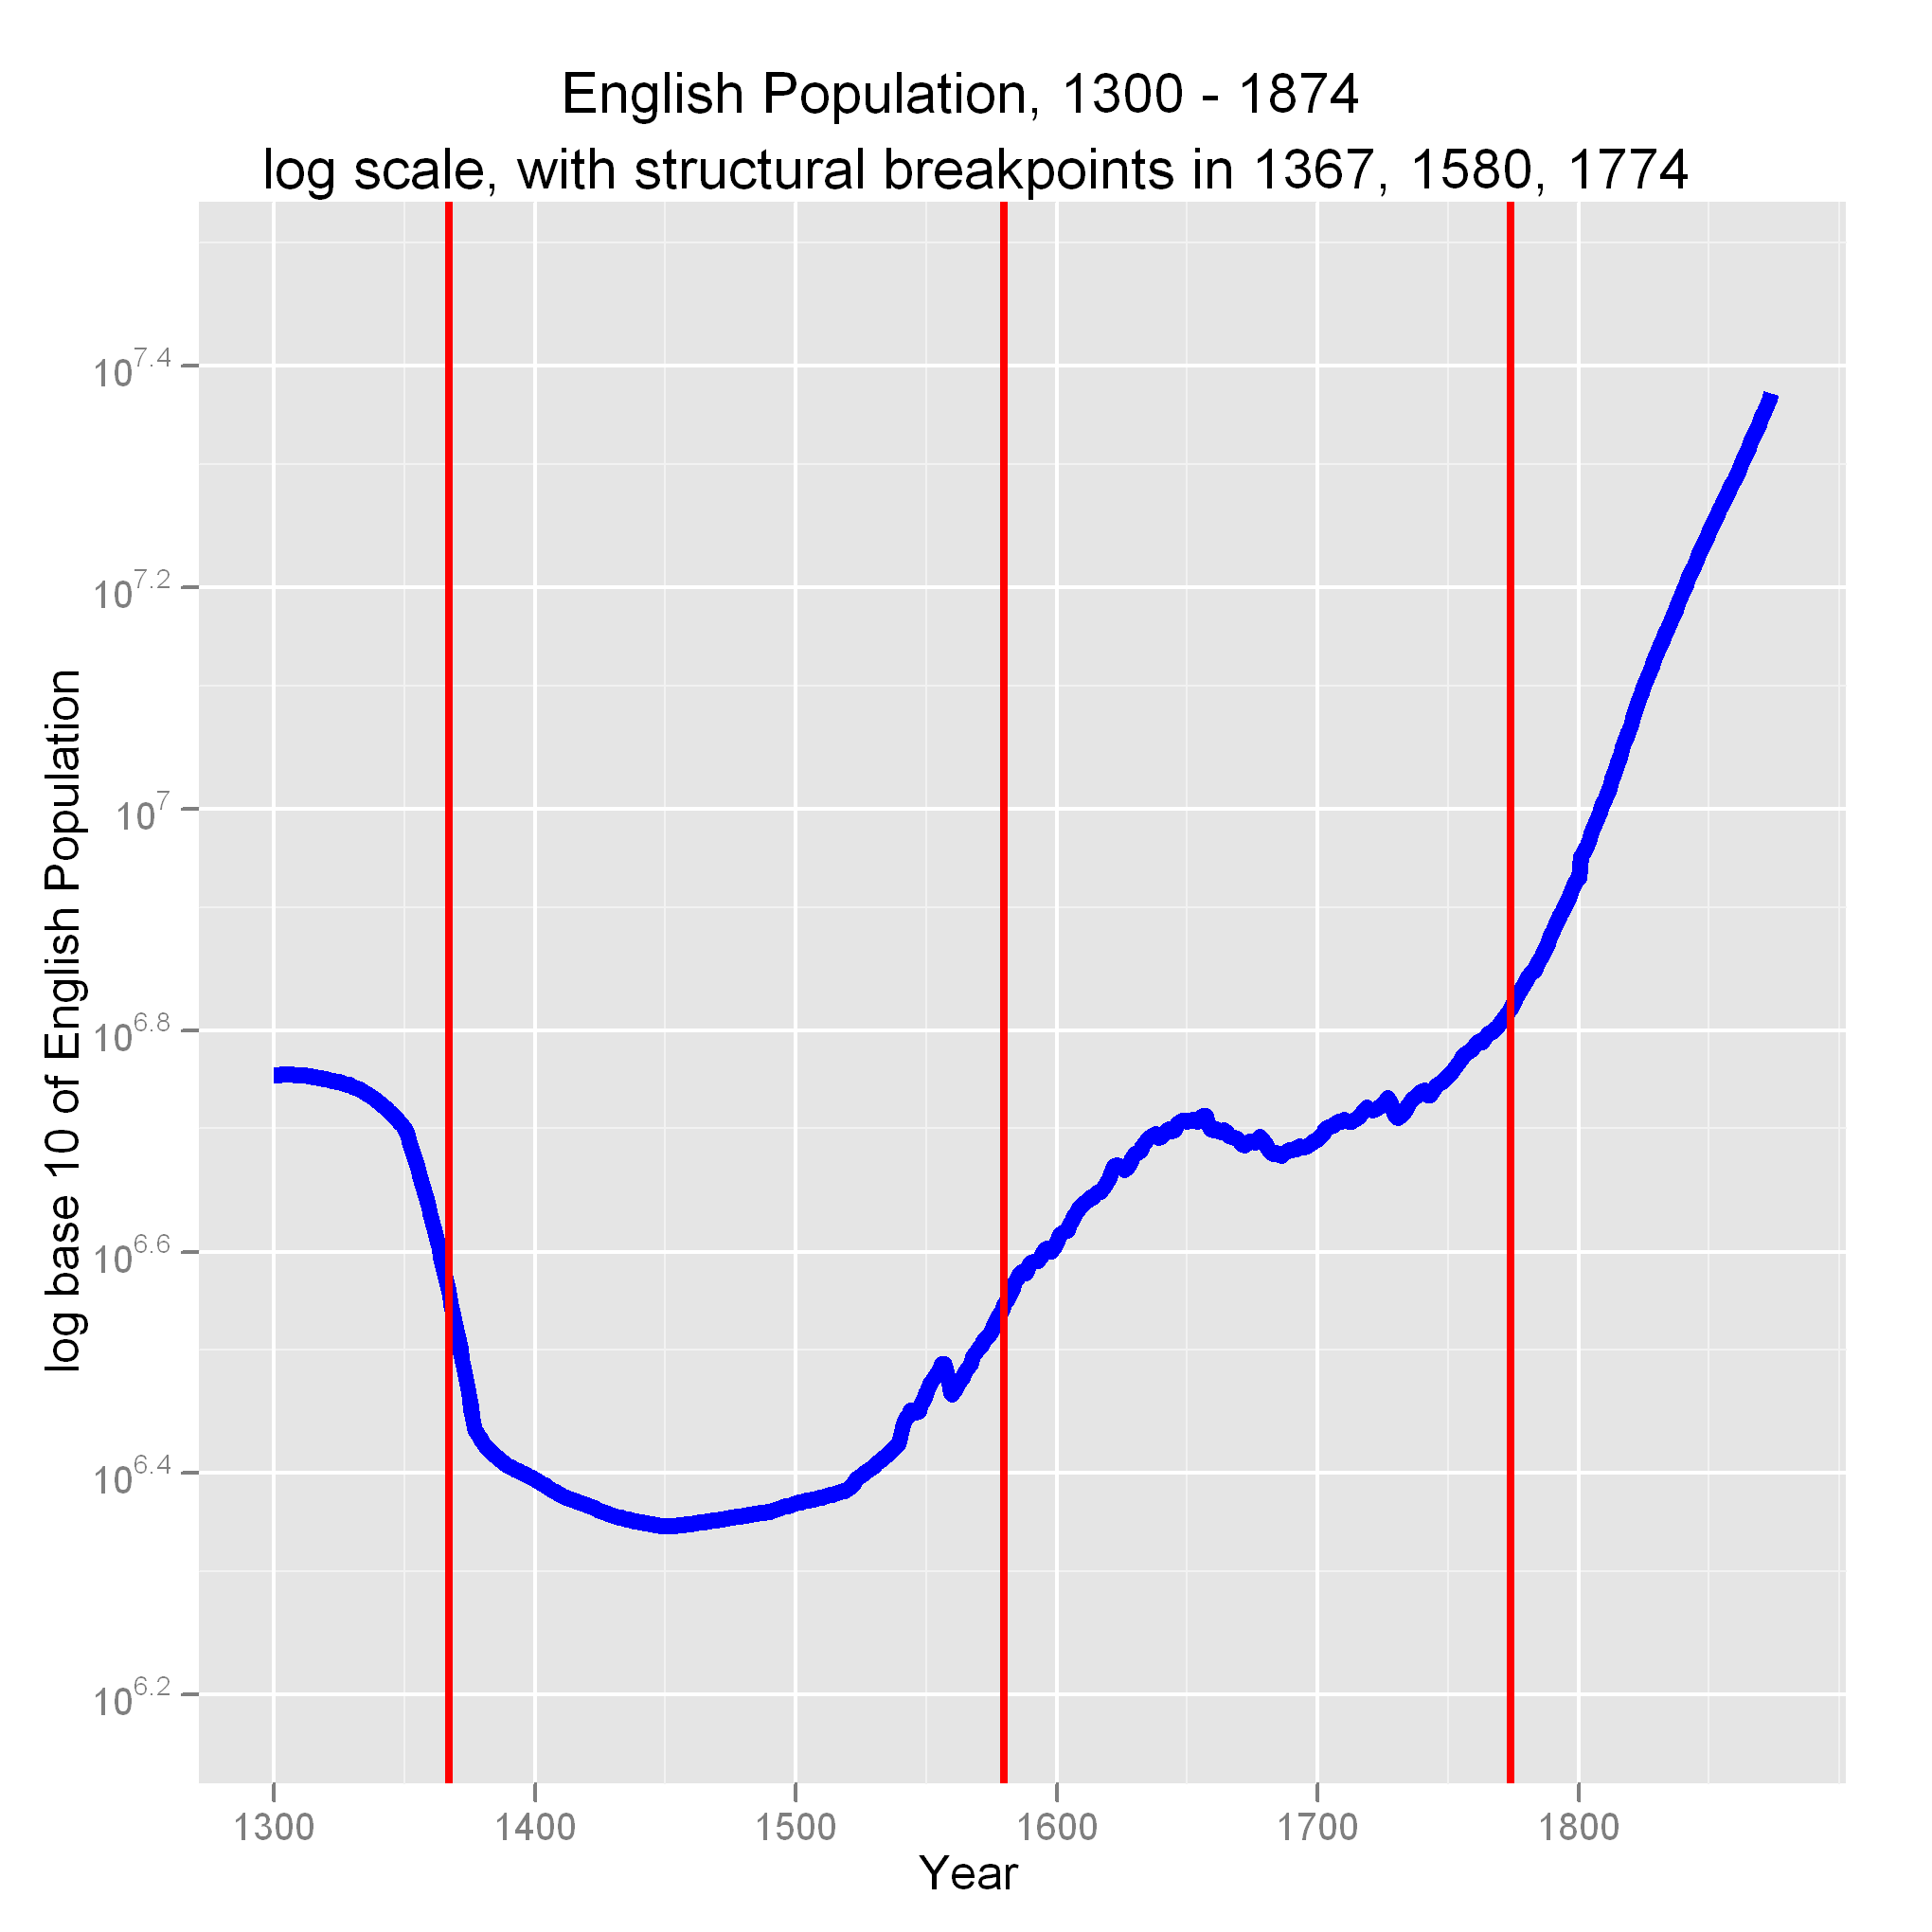
\includegraphics[width=0.39\textwidth]{popLog}}
		}
\end{figure}
\end{frame}

\begin{frame}
\frametitle{Coal and wood energy sources\\\textit{Source:} Pearson \& Fouquet}
\begin{figure}[p!]
\center
%\caption{Coal and wood energy sources\\\textit{Source:} Pearson \& Fouquet}
\label{fig:woodCoal}
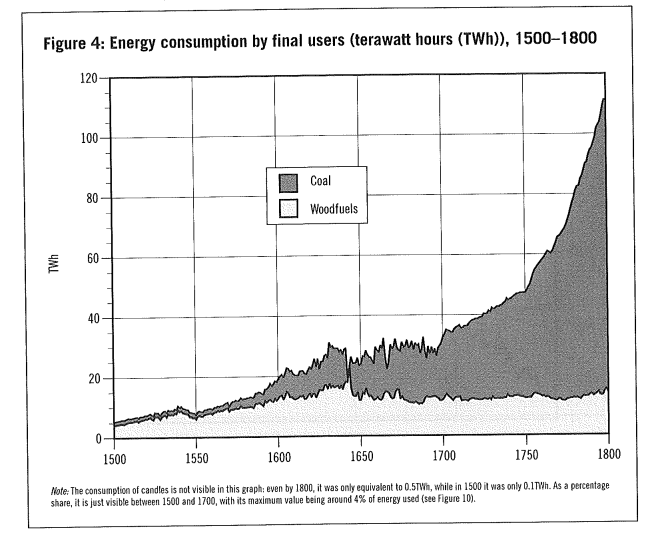
\includegraphics[height=0.8\textheight]{woodCoal.png}
\end{figure}
\end{frame}

\begin{frame}
\frametitle{Energy consumption vs. standarized GDP}
\begin{figure}[p!]
\center
%\caption{Energy consumption vs. standarized GDP}
\label{fig:energyVsGdp}
		\centerline{
		\mbox{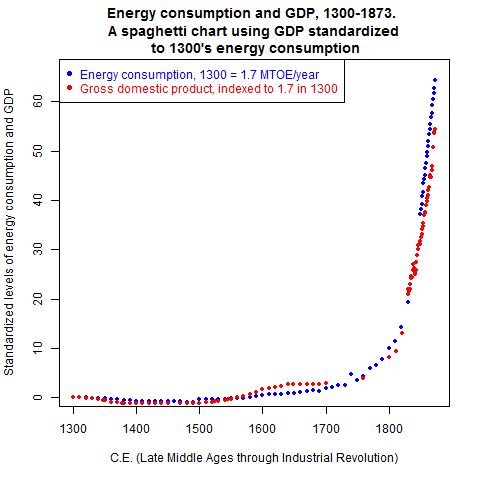
\includegraphics[width=0.55\textwidth]{energyVsGdp}}
		\mbox{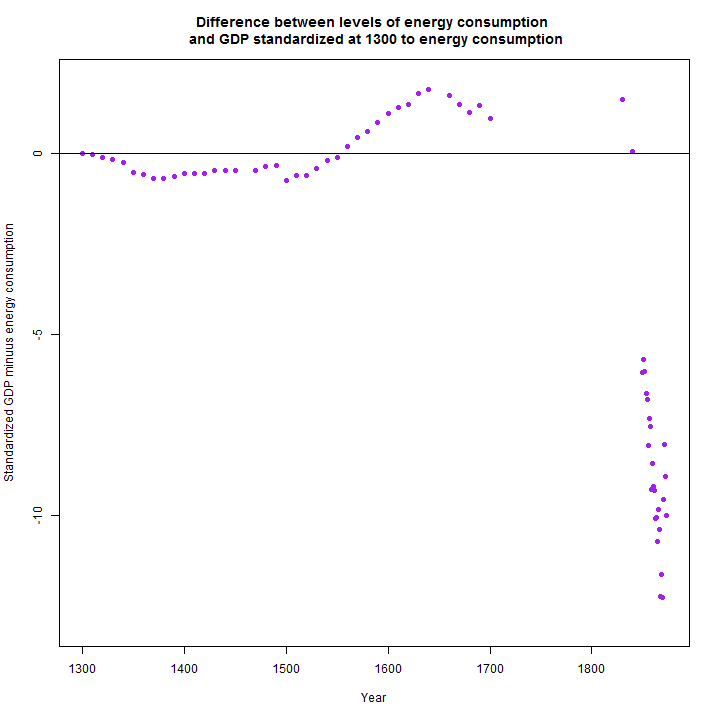
\includegraphics[width=0.55\textwidth]{energyVsGdpDiff}}
		}
\end{figure}
\end{frame}


\begin{frame}
\frametitle{Granger tests of energy/GDP dynamics}
\scriptsize{
\begin{table}[p!]
%\caption{Granger tests of energy/GDP dynamics}
\label{tbl:grangerEnergyGdp}
\begin{tabular}{lrrl}
Era&Energy $\sim$ GDP Pr($>$F)& GDP $\sim$ Energy Pr($>$F)&AS/AD regime\\
\hline \hline
1300 -- 1500&0.0106&0.0003&EMP \footnote{European marriage pattern (Hajnal)}, Black Death: \\&&&increasing wages, \\
&&&family income\\
1500 -- 1600&0.1939&0.6126&Positive demand shock\\
1600 -- 1750&0.3529&0.5185&Energy supply constraint\\
1750 -- 1873&0.0024&0.1100&Positive supply shock:\\&&&``virtuous'' macro \\
&&&feedback cycle\\
\hline
1300 -- 1873& 0.0002& 0.0361&Total study period\\
\end{tabular}
\end{table}
}
\end{frame}

\begin{frame}
\frametitle{English wood energy supply constraint}
\begin{figure}[p!]
\center
%\caption{English wood enegy supply constraint}
\label{fig:wood}
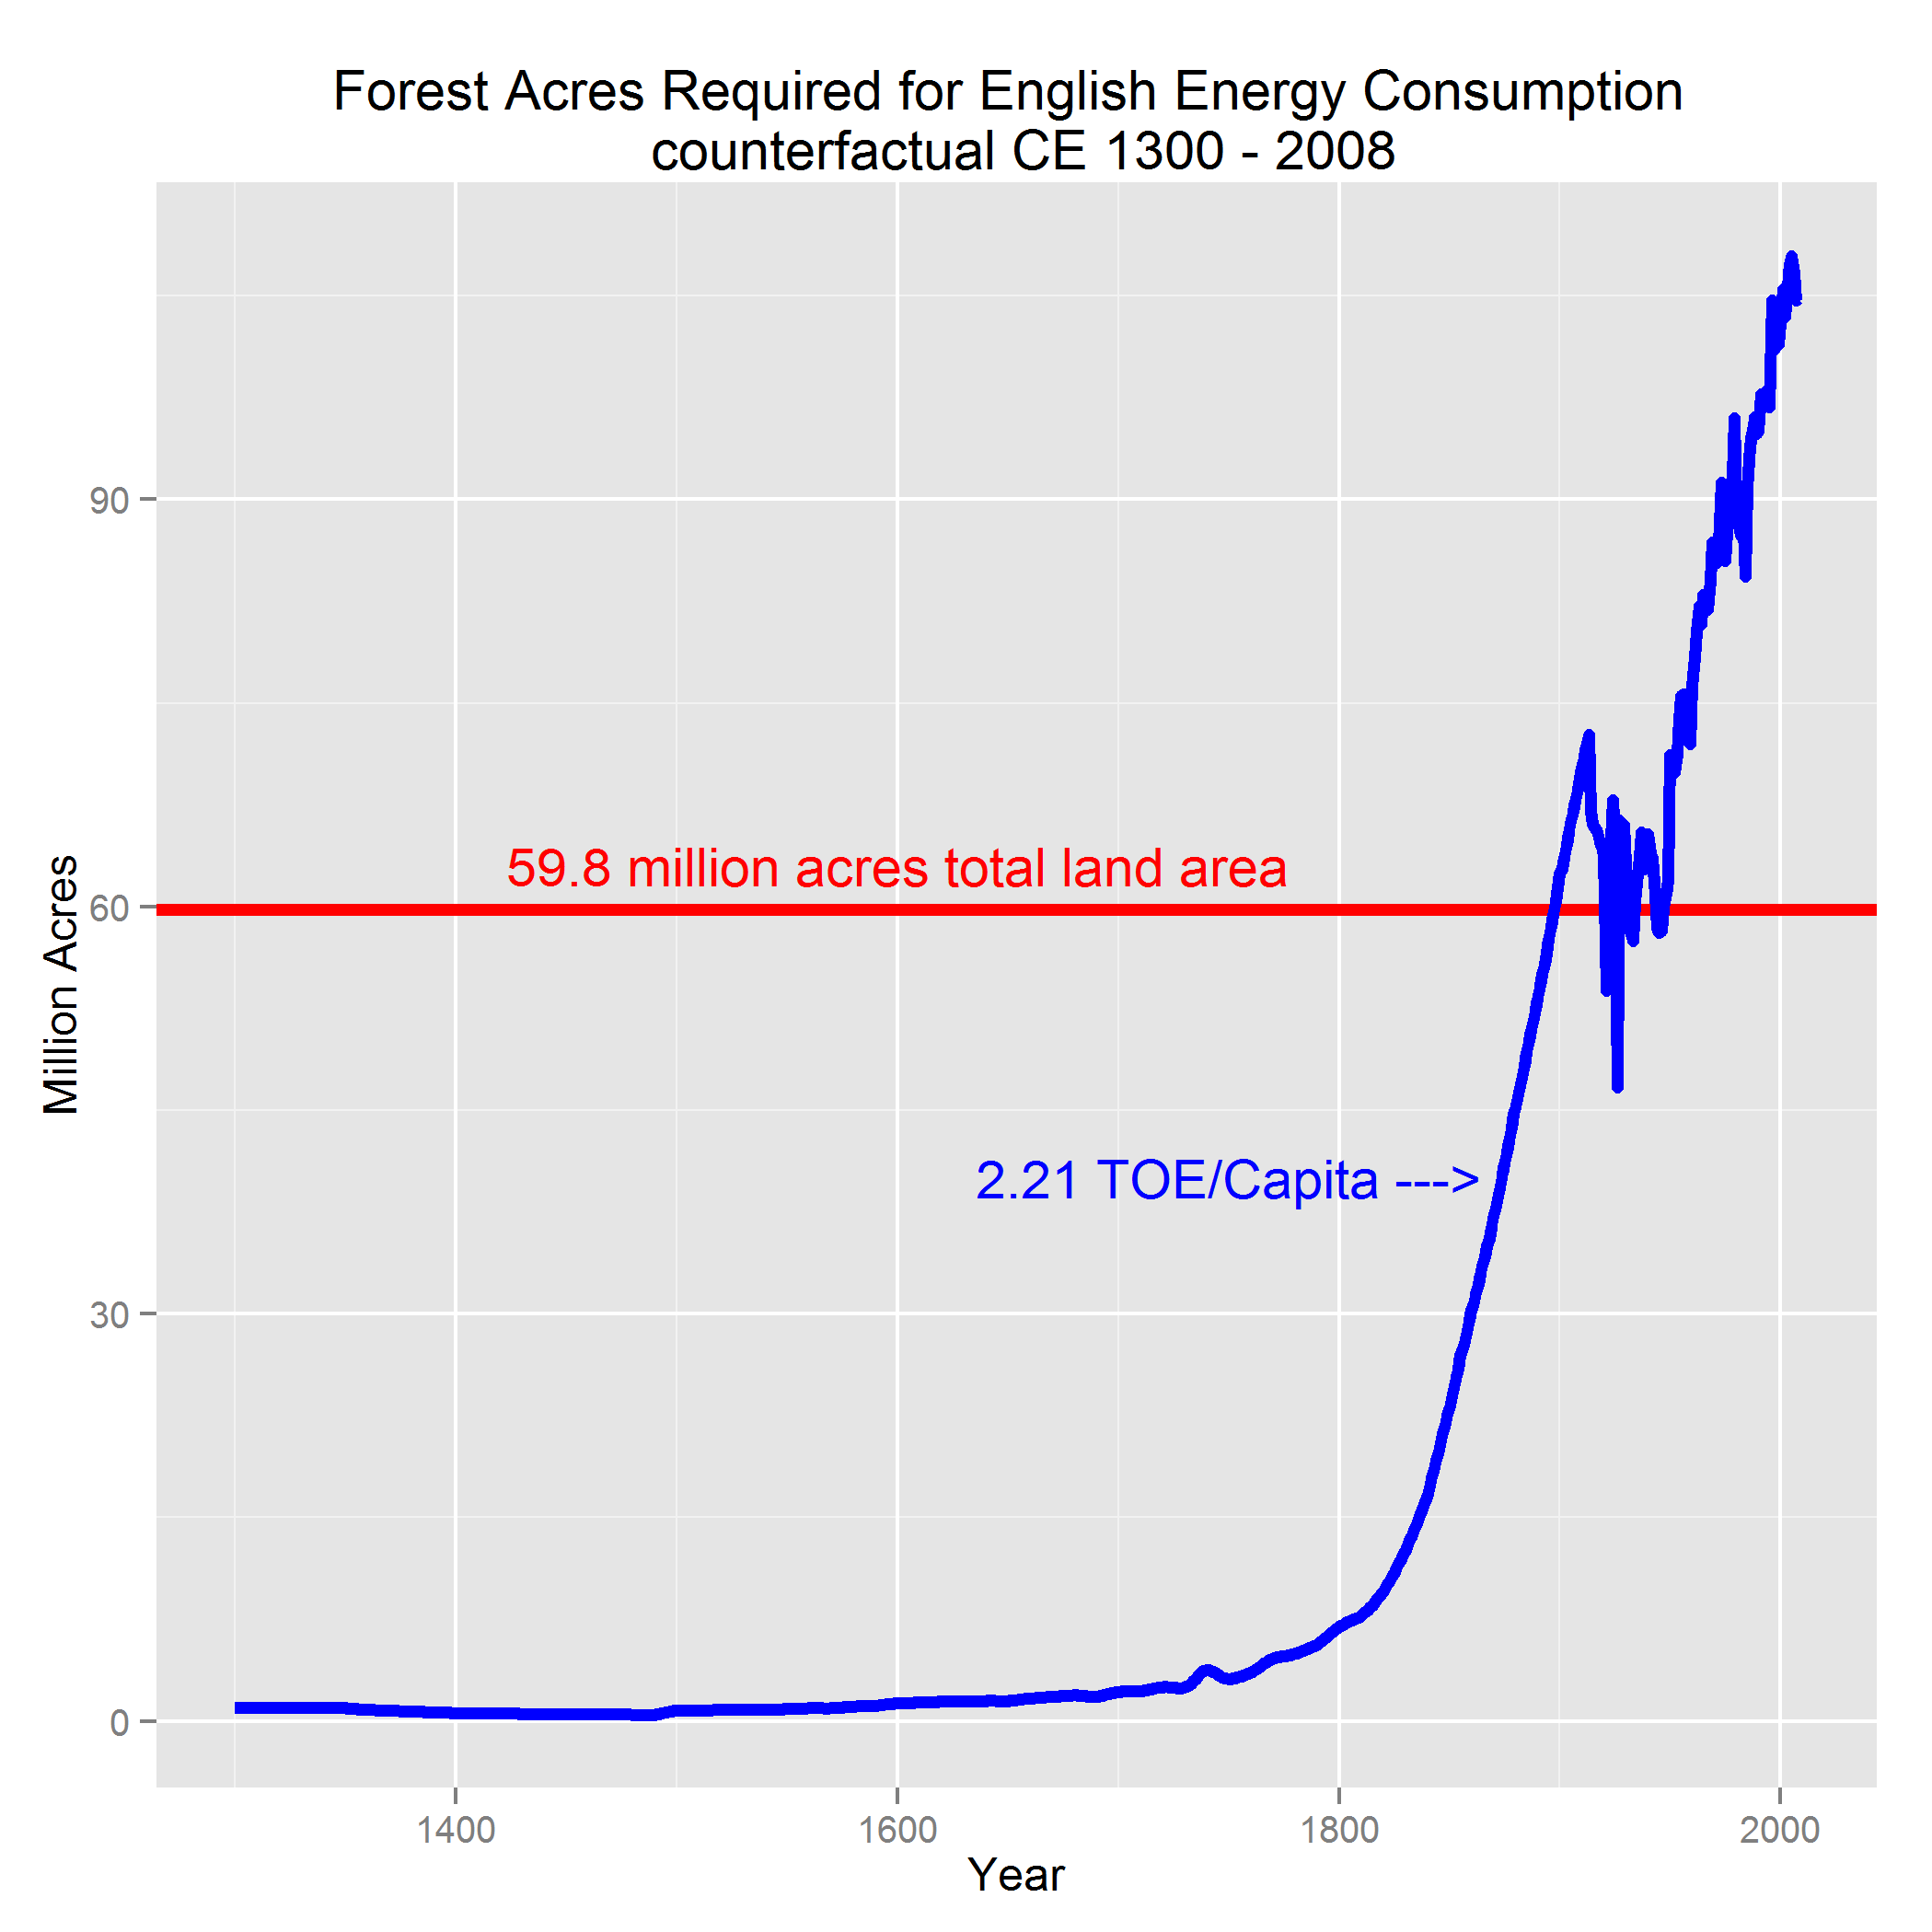
\includegraphics[height=0.8\textheight]{wood}
\end{figure}
\end{frame}

\begin{frame}
\begin{figure}[p!]
\center
\caption{Standardized English energy intensity of GDP}
\label{fig:energyIntensity}
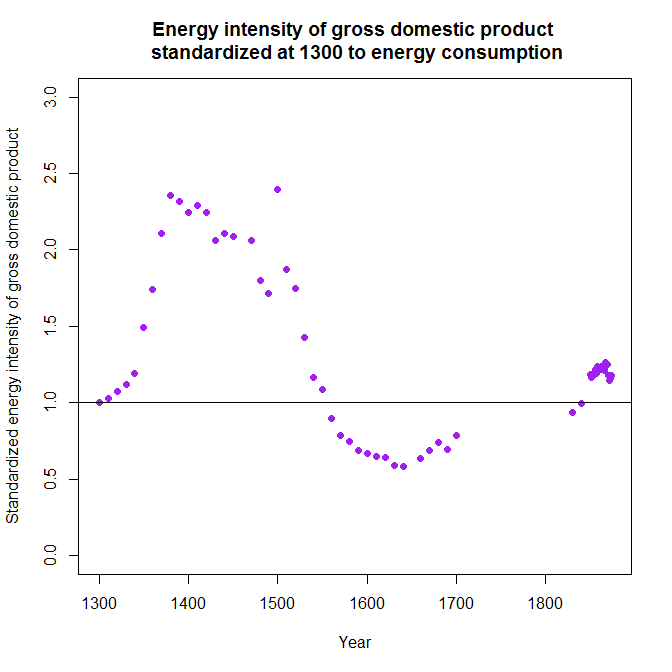
\includegraphics[height=0.8\textheight]{energyIntensity}
\end{figure}
\end{frame}

\begin{frame}
\begin{figure}[p!]
\center
\caption{Log of GDP, with structural breaks}
\label{fig:gbpgdplog.png}
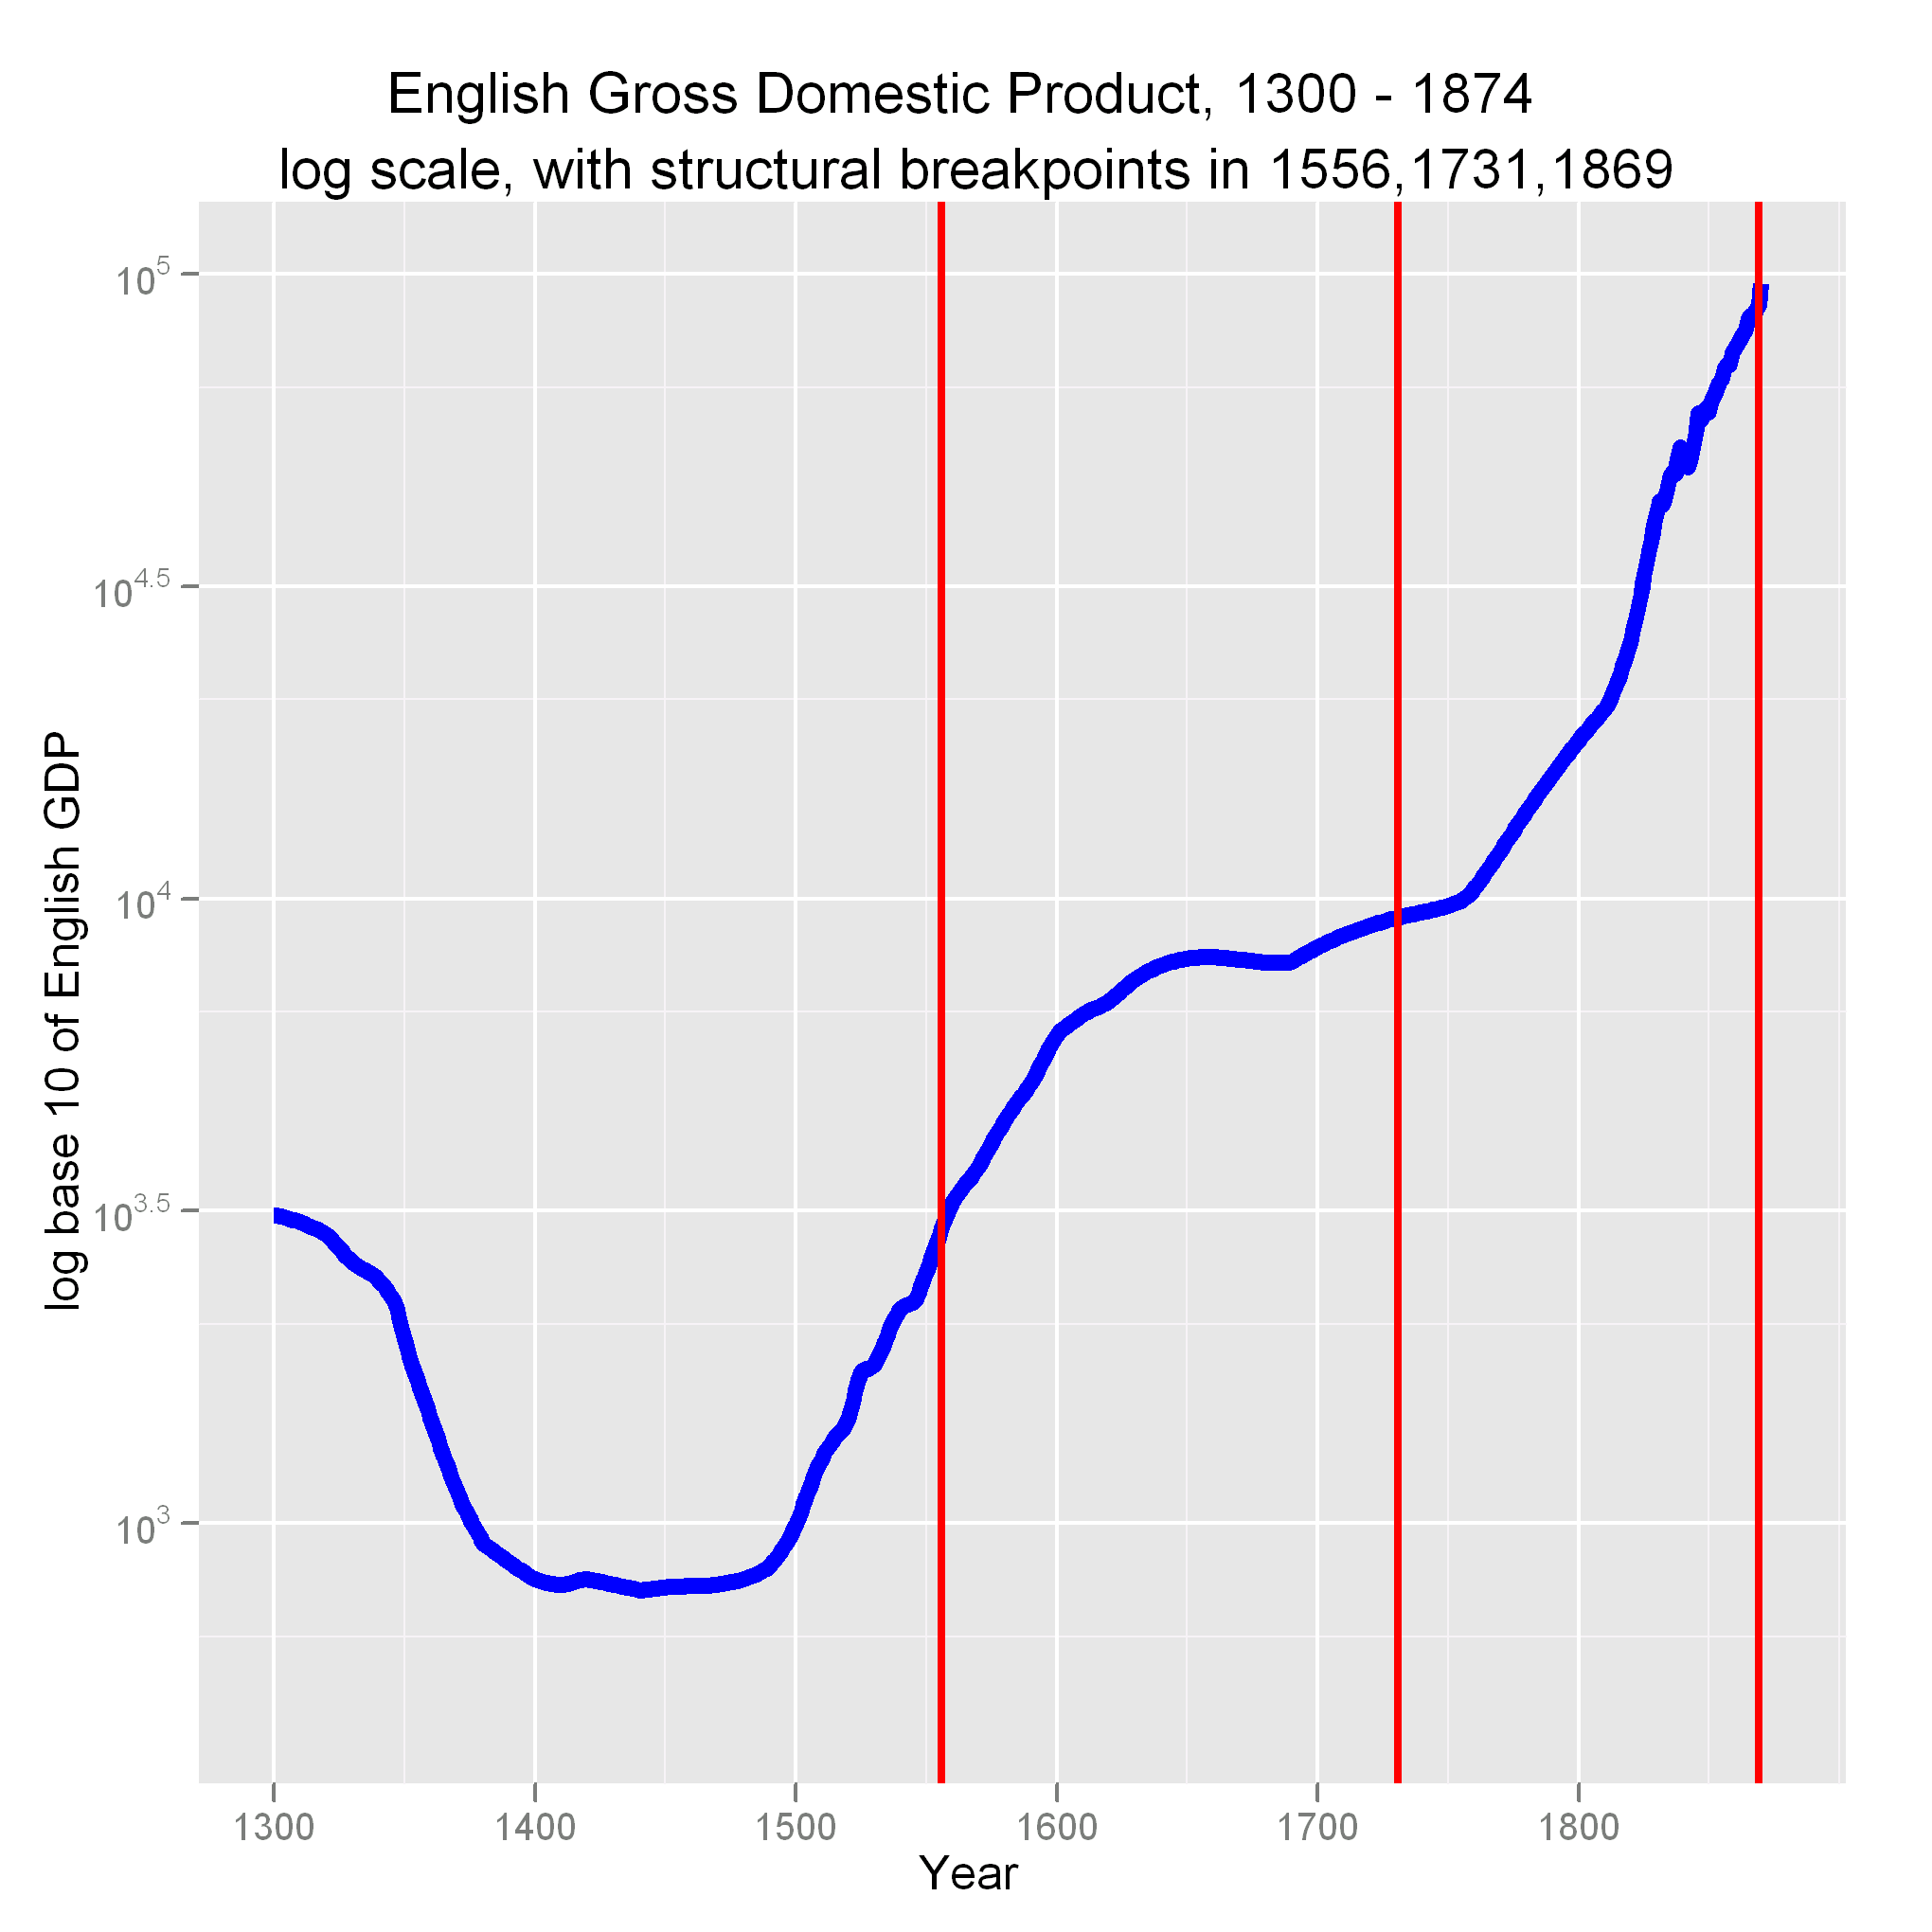
\includegraphics[height=0.8\textheight]{gbpgdplog.png}
\end{figure}
\end{frame}

\begin{frame}
\begin{figure}[p!]
\center
\caption{Log of population, with structural breaks}
\label{fig:popLog}
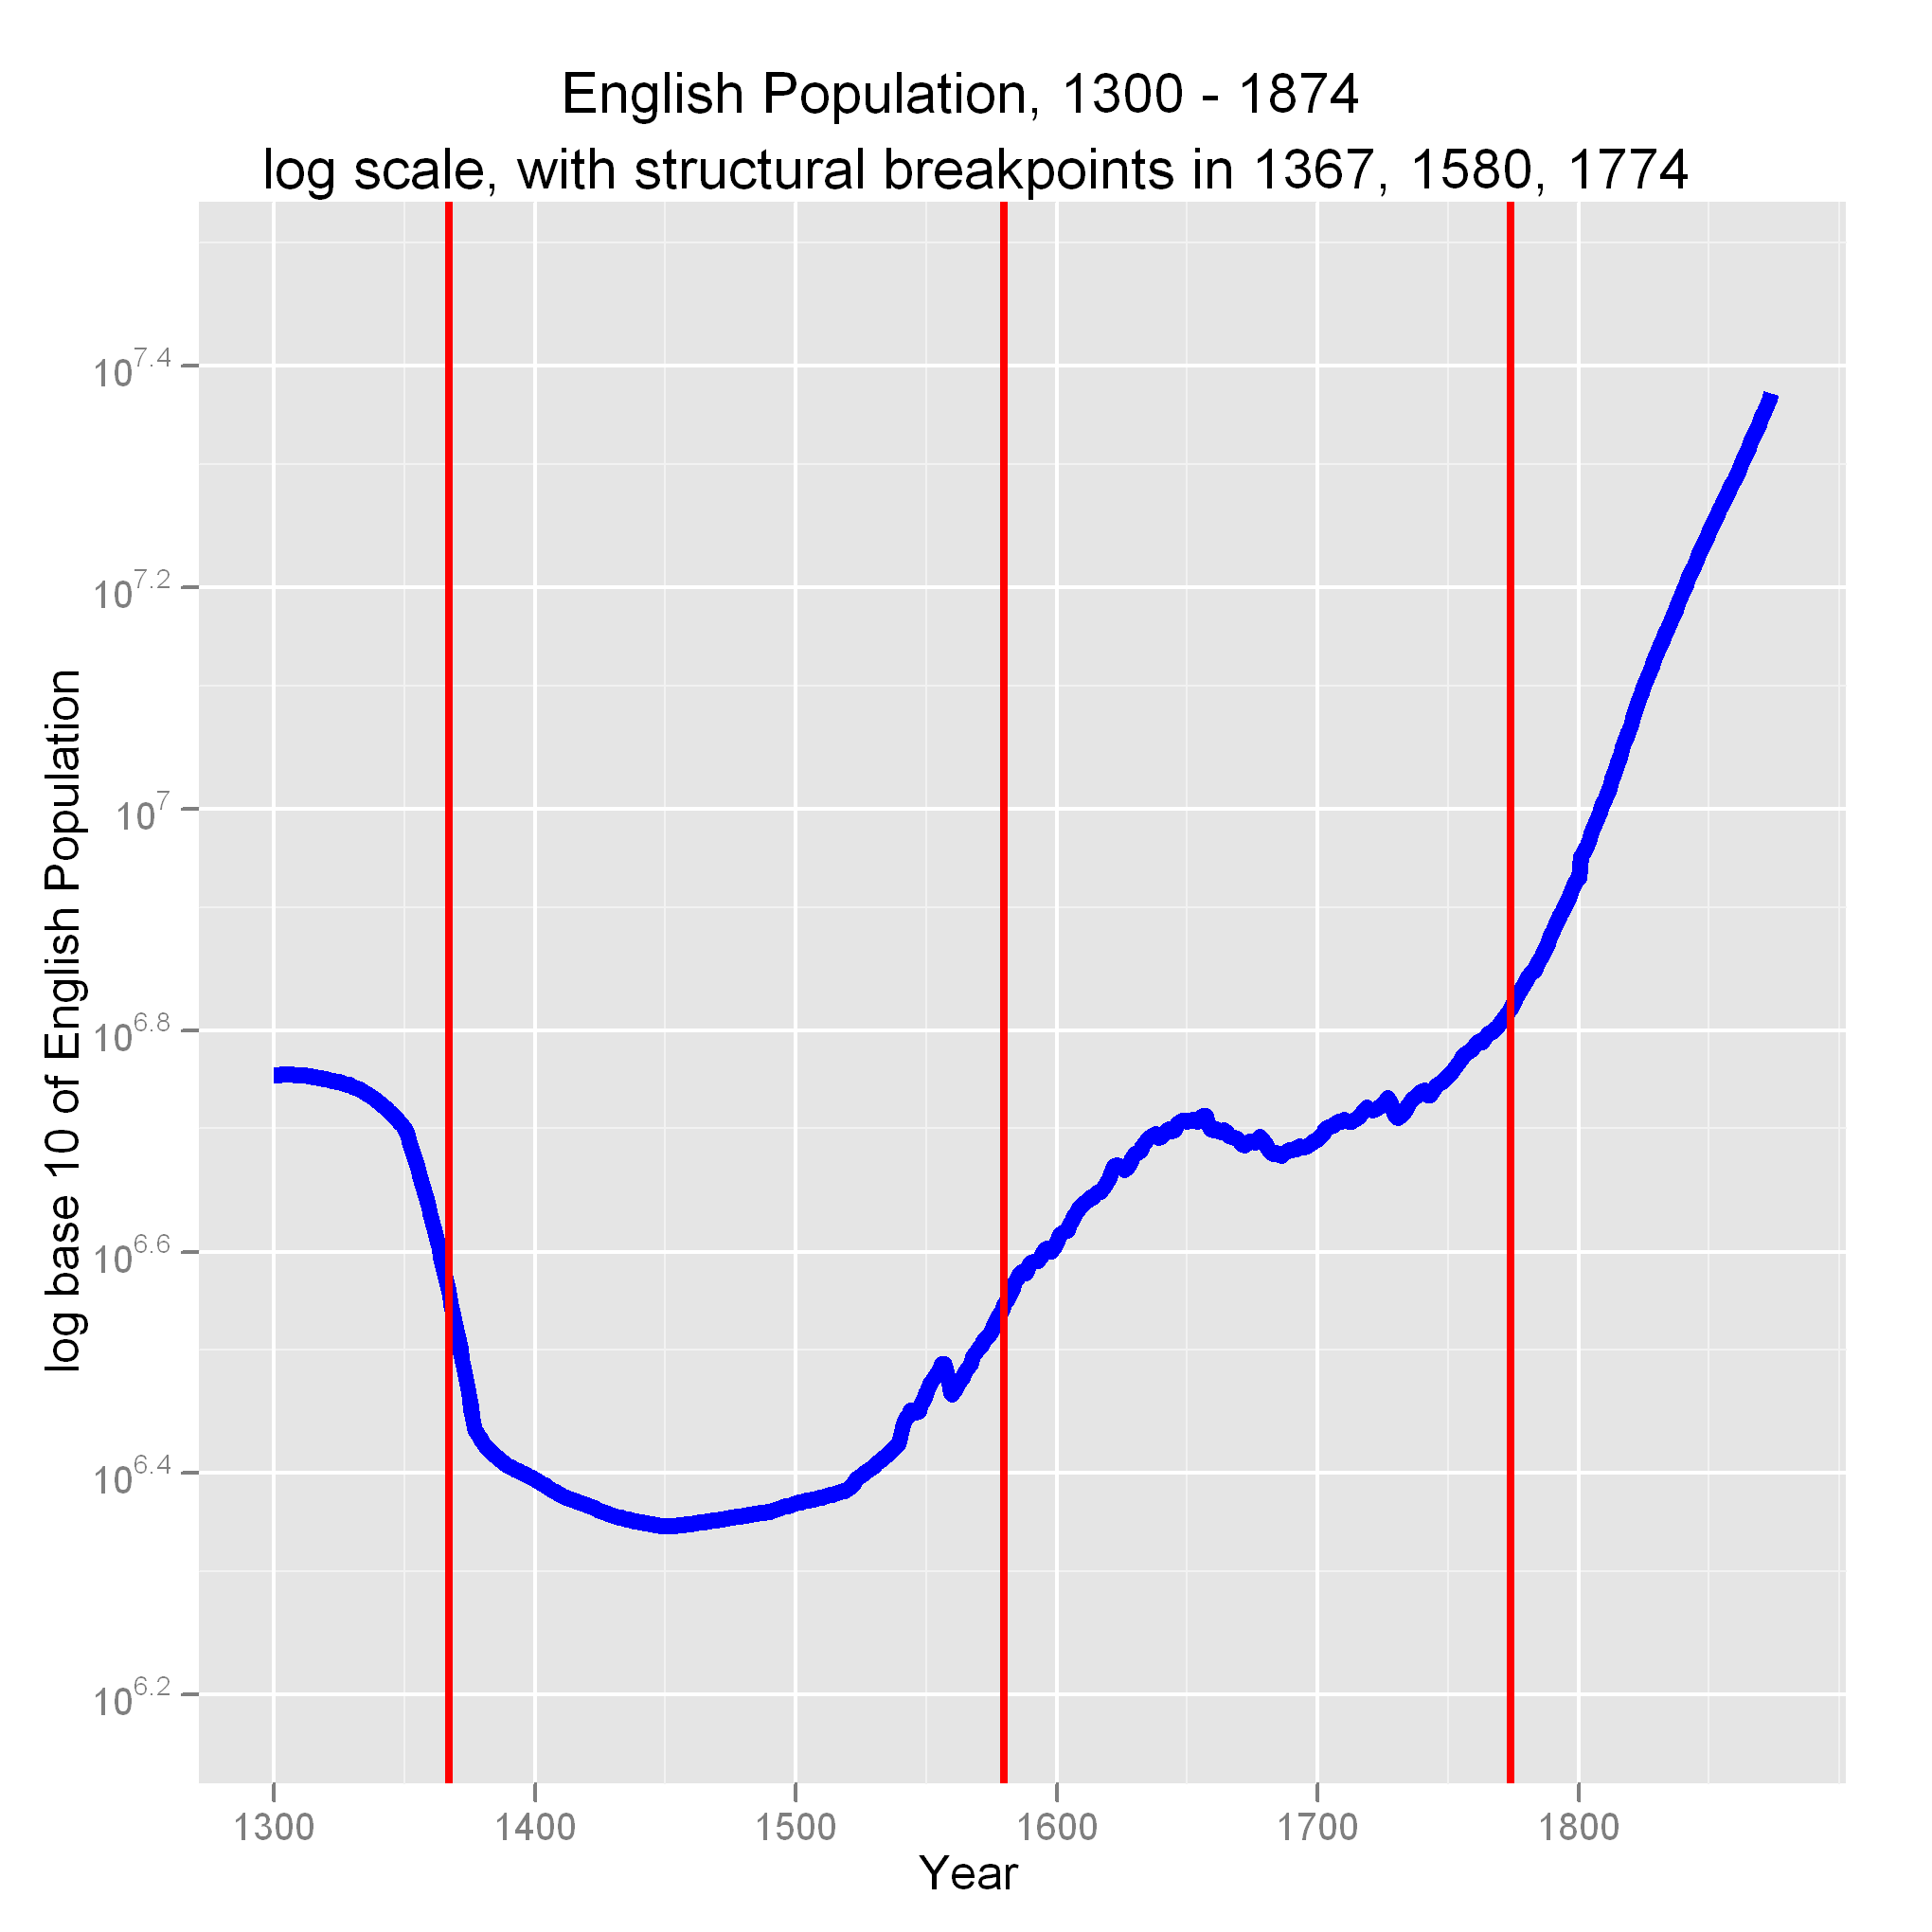
\includegraphics[height=0.8\textheight]{popLog}
\end{figure}
\end{frame}

\begin{frame}
\frametitle{Data Sources}
\footnotesize{
\begin{table}[p!]
%\caption{Data Sources}
\label{tbl:dataSources}
\begin{tabular}{lrll}
Data series&Year range&Geography&Source\\
\hline
Energy consumption&1300 -- 1873&England/Wales&Roger Fouquet (2008)\\
\hline
Gross domestic product&1300 -- 1700&England&Graeme Snooks (1994)\\
&1741 -- 1873&England/Wales&Lawrence Officer (2009)\\
\hline
Population&1300 -- 1540&England&Graeme Snooks (1994)\\
&1541 -- 1800&England&B. R. Mitchell (1988)\\
&1801 -- 1873&England/Wales&B. R. Mitchell (1988)\\
\end{tabular}
\end{table}
}
\end{frame}

\begin{comment}
\begin{table}[p!]
\caption{t-test of energy and gdp}
\label{tbl:t-testEnergyGdp}
\begin{tabular}{rl}
\end{tabular}
\end{table}
\end{comment}

\begin{frame}
\tiny{
\begin{table}[p!]
\caption{growth rates by century}
\label{tbl:growthByCentury}
\begin{tabular}{lrrrrrrrr}
Year	&	1300	&	1400	&	1500	&	1600	&	1700	&	1801	&	1873&Total	\\
\hline
GDP Million\\ 2005 GBP	&	3114.7541	&	815.1288	&	994.4571	&	6031.953	&	8361.5911	&	18110	&	102811&	\\
Century-over-century\\rate of growth&&-0.738&0.220&5.066&0.386&1.166&4.677&32.008\\
Compounded annual \\rate of growth&&-0.013&0.002&0.018&0.003&0.008&0.024&0.006\\
\hline
Energy consumption&1.7	&	1	&	1.3	&	2.2	&	3.6	&	11.6	&	66.1&	\\
Century-over-century\\rate of growth&&-0.412&0.300&0.692&0.636&2.222&4.698&37.882\\
Compounded annual \\rate of growth&&-0.005&0.0026&0.005&0.005&0.012&0.024&0.006\\
\hline
Per-capita GDP\\2005 GBP&542&  329&  421& 1,484& 1,663& 1,999& 4,392\\
Century-over-century\\rate of growth&&-0.393& 0.282&2.521&0.121&0.202&1.198& 7.108\\
Compounded annual \\rate of growth&&-0.005&0.002&0.013&0.001&0.002& 0.011&0.004\\
\end{tabular}
\end{table}
}
\end{frame}

\begin{frame}
\begin{table}[p!]
\caption{Energy and GDP fit tests}
\label{tbl:fitTest}
\begin{center}
\begin{tabular}{lrr}
\hline\hline
Test&Statistic&p-value\tabularnewline
\multicolumn{1}{c}{}\tabularnewline
\hline
Pearson's correlation&$0.998$&\tabularnewline
\hline
Paired t-test&$5.592$&4.991e-07\tabularnewline
\hline
Chi-square&2864&0.0004998\tabularnewline
\end{tabular}
\end{center}
\end{table}
\end{frame}

\begin{frame}
\frametitle{Engels -- Socialism: Utopian and Scientific (1880)}
\centering III
\centering [Historical Materialism]
\tiny{
The materialist conception of history starts from the proposition that the production of the means to support human life and, next to production, the exchange of things produced, is the basis of all social structure; that in every society that has appeared in history, the manner in which wealth is distributed and society divided into classes or orders is dependent upon what is produced, how it is produced, and how the products are exchanged. From this point of view, the final causes of all social changes and political revolutions are to be sought, not in men's brains, not in men's better insights into eternal truth and justice, but in changes in the modes of production and exchange. They are to be sought, not in the philosophy, but in the economics of each particular epoch. The growing perception that existing social institutions are unreasonable and unjust, that reason has become unreason, and right wrong [1], is only proof that in the modes of production and exchange changes have silently taken place with which the social order, adapted to earlier economic conditions, is no longer in keeping. From this it also follows that the means of getting rid of the incongruities that have been brought to light must also be present, in a more or less developed condition, within the changed modes of production themselves. These means are not to be invented by deduction from fundamental principles, but are to be discovered in the stubborn facts of the existing system of production.
}
\end{frame}

\end{document}